\subsection[NGEE Arctic]{Next-Generation Ecosystem Experiments (NGEE Arctic)}
%%%%%%%%%%%%%%%%%%%%%%%%%%%%%%%%%%%%%%%%%%%%%%%%%%%%%%%%%%%%%%%%%%%%%%%%%%%%%%%
\begin{frame}
 \begin{center}
  \vskip-0.15in
  \begin{block}{}\centering
   \textbf{\color{CCSIGreen}Next-Generation Ecosystem Experiments (NGEE Arctic) \\
   \url{http://ngee.ornl.gov/}}
  \end{block}
  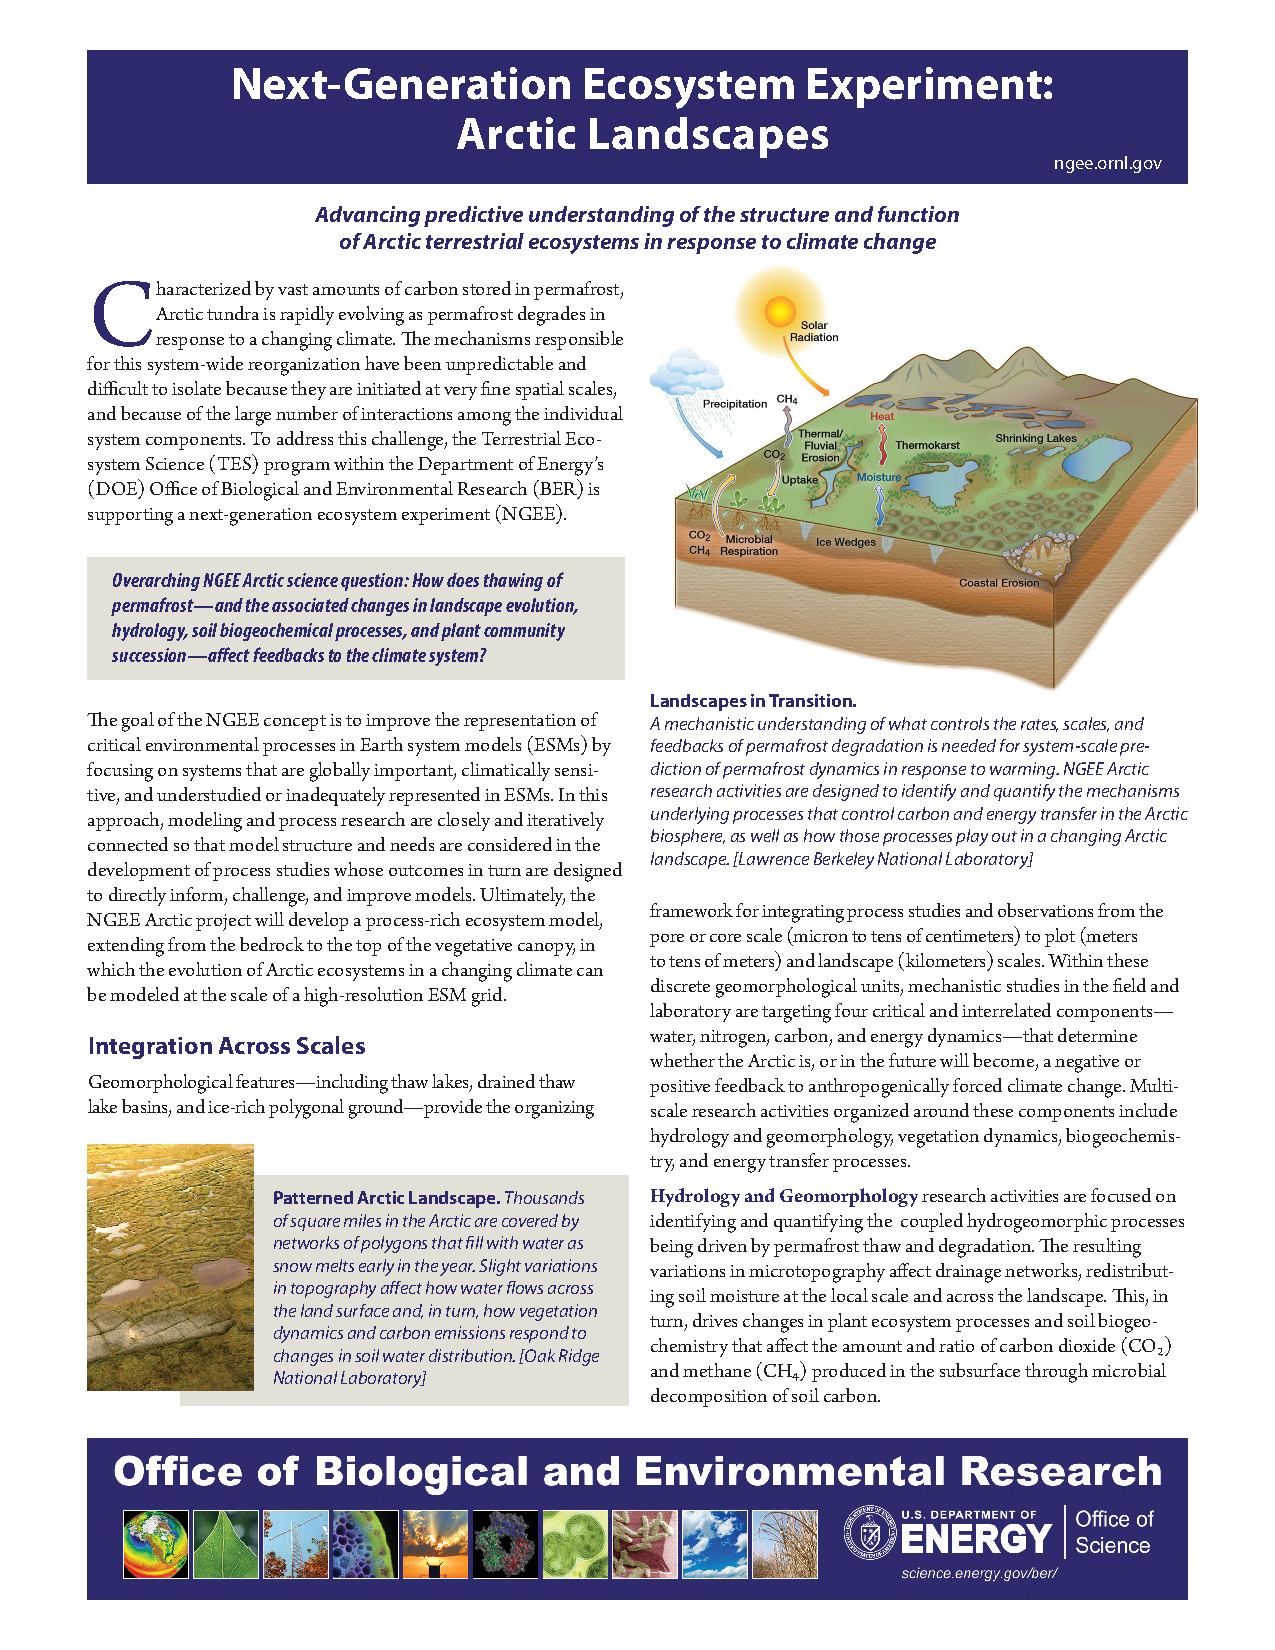
\includegraphics[width=0.74\textwidth,page=1,trim=4.25in 6.38in 0.5in 1.75in,clip=TRUE]{ngee_figures/TES-ArcticEco_07-25-2012d.pdf} \\
  %\vskip-0.25in
  \tiny\textit{The Next-Generation Ecosystem Experiments (NGEE Arctic) project is
supported by the Office of Biological and Environmental Research in the
DOE Office of Science.
}
 \end{center}
 \vskip-0.25in
 \begin{block}{}
  {
\includegraphics[height=0.05\paperheight]{logos/DOE_logo.png}\hfill
\includegraphics[height=0.07\paperheight]{logos/ORNL_logo.png}\hfill
\includegraphics[height=0.07\paperheight]{logos/LANL_logo.png}\hfill
\includegraphics[height=0.07\paperheight]{logos/LBNL_logo.png}\hfill
\includegraphics[height=0.07\paperheight]{logos/BNL_logo.png}\hfill
\includegraphics[height=0.07\paperheight]{logos/UAF_logo.png}}
 \end{block}
\end{frame}
%%%%%%%%%%%%%%%%%%%%%%%%%%%%%%%%%%%%%%%%%%%%%%%%%%%%%%%%%%%%%%%%%%%%%%%%%%%%%%%
\begin{frame}
 \frametitle{Integrating Across Scales}
 \begin{itemize}\small
  \item NGEE Arctic process studies and observations are strongly linked to model development and application for improving process representation, initialization, calibration, and evaluation.
  \item A hierarchy of models will be deployed at fine, intermediate, and climate scales to connect observations to models and models to each other in a quantitative up-scaling and down-scaling framework.
\end{itemize}
\begin{center}
  \includegraphics[width=\textwidth,page=2,trim=0.58in 7.75in 0.58in 0.325in,clip=TRUE]{ngee_figures/TES-ArcticEco_07-25-2012d.pdf} \\
 \end{center}
\end{frame}
%%%%%%%%%%%%%%%%%%%%%%%%%%%%%%%%%%%%%%%%%%%%%%%%%%%%%%%%%%%%%%%%%%%%%%%%%%%%%%%%
%
%
%%%%%%%%%%%%%%%%%%%%%%%%%%%%%%%%%%%%%%%%%%%%%%%%%%%%%%%%%%%%%%%%%%%%%%%%%%%%%%%
\subsection[Representativeness]{Representativeness-Based Network Design}
%\section{Introduction}
%%%%%%%%%%%%%%%%%%%%%%%%%%%%%%%%%%%%%%%%%%%%%%%%%%%%%%%%%%%%%%%%%%%%%%%%%%%%%%%
% NGEE-Arctic Site-representativeness introduction slide
%%%%%%%%%%%%%%%%%%%%%%%%%%%%%%%%%%%%%%%%%%%%%%%%%%%%%%%%%%%%%%%%%%%%%%%%%%%%%%%
%
%%
%% HOPEFULLY, slides motivating the need for the NGEE project itself will have
%% been presented for this last set of slides for the last 15 minutes of
%% tag-team presentations.
%%
%%\begin{frame}{Representativeness and Scaling}
%% \begin{itemize}
%%  \item Need for studies of the complex and interacting processes of the
%%atmosphere, sea ice, ocean, and terrestrial systems in Arctic to improve
%%the interpretation of past climate and projections of future climate.
%%  \item Committee on Designing an Arctic Observing Network  recommended an
%%Arctic Observing Network to satisfy current and future scientific by
%%monitoring key physical, biogeochemical, and human dimensions
%%variables.
%%  \item Conducting systematic and continuous field observations and long
%%term monitoring are challenging, particularly in the Arctic.
%% \end{itemize}
%%\end{frame}
%%
%
\begin{frame}
 %\frametitle{Representativeness and Scaling}
 \frametitle{Quantitative Sampling Network Design}
 \begin{itemize}
  \item Resource and logistical constraints limit the frequency and extent
  of observations, necessitating the development of a systematic sampling
  strategy that objectively represents environmental variability at the
  desired spatial scale.
  \item Required is a methodology that provides a quantitative framework
  for informing site selection and determining the representativeness
  of measurements.
  \item Multivariate spatiotemporal clustering (MSTC) was applied at
  the landscape scale (4~km$^2$) for the State of Alaska to demonstrate
  its utility for representativeness and scaling.
  \item An extension of the method applied by Hargrove and Hoffman for
  design of National Science Foundation's (NSF's) National Ecological
  Observatory Network (NEON) domains \citep{Schimel_FrontEcolEnviron_20070301,Keller_FrontEcolEnviron_20080601}.
 \end{itemize}

\end{frame}


%%%%%%%%%%%%%%%%%%%%%%%%%%%%%%%%%%%%%%%%%%%%%%%%%%%%%%%%%%%%%%%%%%%%%%%%%%%%%%%
\begin{frame}{Multivariate Spatiotemporal Clustering (MSTC)}
 \vskip-0.15in
 \begin{figure}
  \begin{center}
   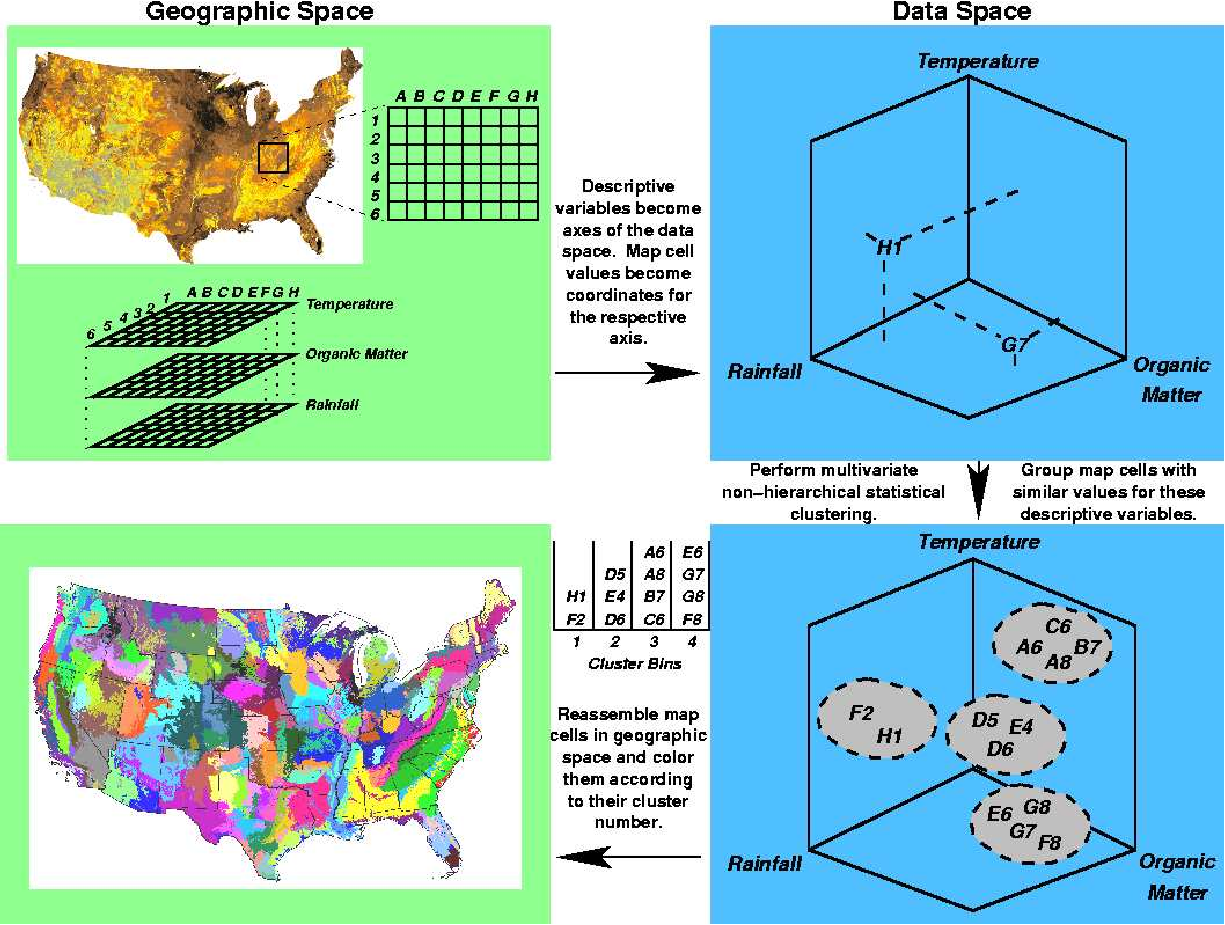
\includegraphics[width=0.91\textwidth]{ngee_figures/clusterfinal3}
  \end{center}
  %\caption{Cluster analysis.}
%  \label{fig:clusterfinal3}
 \end{figure}
\end{frame}
%%%%%%%%%%%%%%%%%%%%%%%%%%%%%%%%%%%%%%%%%%%%%%%%%%%%%%%%%%%%%%%%%%%%%%%%%%%%%%%

\subsection{Data Layers}

%%%%%%%%%%%%%%%%%%%%%%%%%%%%%%%%%%%%%%%%%%%%%%%%%%%%%%%%%%%%%%%%%%%%%%%%%%%%%%%
\begin{frame}{Data Layers}\footnotesize
 \begin{table}
 \vskip-0.15in
 \scriptsize%\tiny
  \caption{37 variables averaged for 2000--2009 and 2090--2099}\label{tbl:characteristics}
  \centering
  \begin{tabular}{m{4.2cm}ccc}
   \toprule
   Description & Number/Name & Units & Source \\
   \midrule
   Monthly mean air temperature                   & 12                 & $^\circ$C   & GCM \\
   Monthly mean precipitation                     & 12                 & mm          & GCM \\
   \multirow{2}{*}{Day of freeze}                 & mean               & day of year & GCM \\
                                                  & standard deviation & days        & \\
   \multirow{2}{*}{Day of thaw}                   & mean               & day of year & GCM \\
                                                  & standard deviation & days        & \\
   \multirow{2}{*}{Length of growing season}      & mean               & days        & GCM \\
                                                  & standard deviation & days        & \\
   Maximum active layer thickness                 & 1                  & m           & GIPL \\
   Warming effect of snow                         & 1                  & $^\circ$C   & GIPL \\
   Mean annual ground temperature at bottom of active layer & 1                  & $^\circ$C   & GIPL \\
   Mean annual ground surface temperature         & 1                  & $^\circ$C   & GIPL \\
   Thermal offset                                 & 1                  & $^\circ$C   & GIPL \\
   Limnicity                                      & 1                  & \%          & NHD \\
   Elevation                                      & 1                  & m           & SRTM \\
   \bottomrule
  \end{tabular}
\end{table}


\end{frame}
%%%%%%%%%%%%%%%%%%%%%%%%%%%%%%%%%%%%%%%%%%%%%%%%%%%%%%%%%%%%%%%%%%%%%%%%%%%%%%%

\subsection[Ecoregions]{Alaska Ecoregions}

%%%%%%%%%%%%%%%%%%%%%%%%%%%%%%%%%%%%%%%%%%%%%%%%%%%%%%%%%%%%%%%%%%%%%%%%%%%%%%%
\begin{frame}
 \frametitle{10 Alaska Ecoregions (2000--2009)}
 \begin{figure}
  \begin{center}
   \vskip-0.20in
   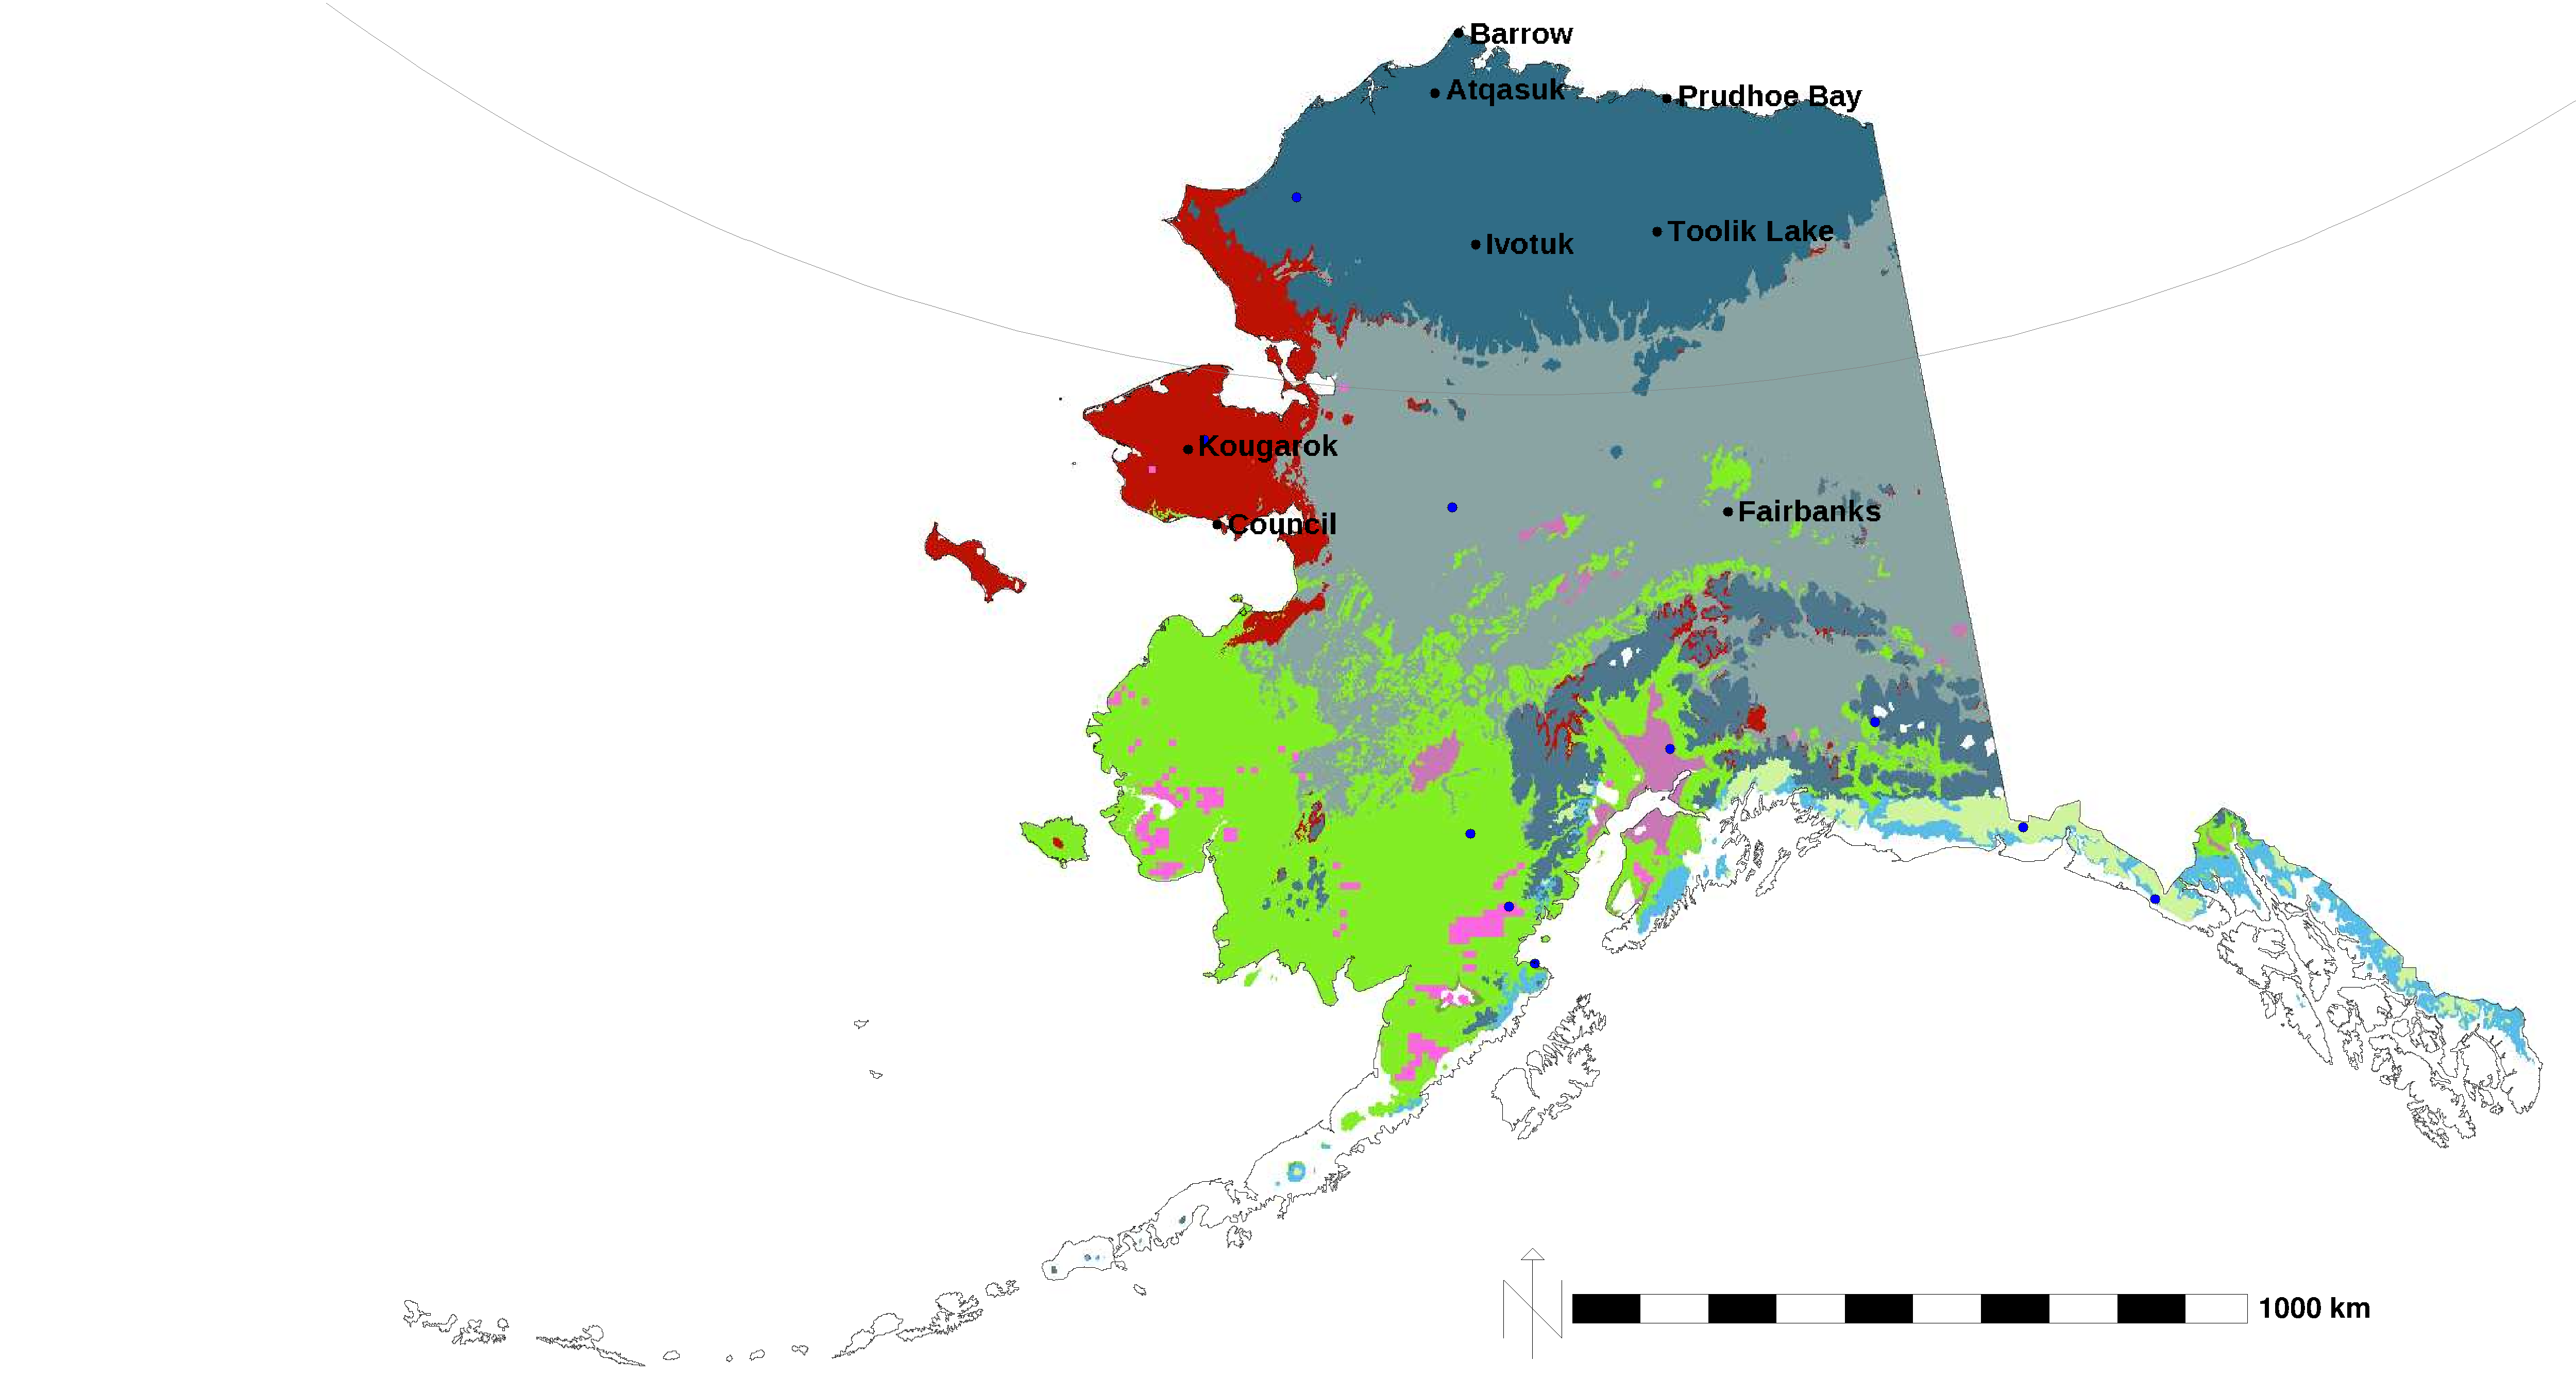
\includegraphics[width=\textwidth]{ngee_figures/alaska_dem_Feb2012_10_2000-2009_barscale}
  \end{center}
  %\caption{Cluster analysis.}
  \label{fig:alaska_2000_2009_10}
 \end{figure}
 \vskip-0.10in
 \vbox{\scriptsize\hfill\citep{Hoffman_LandscapeEcol_20131001}}
\smallskip
Each ecoregion is a different random color. Blue filled circles mark
locations most representative of mean conditions of each region.
\end{frame}
%%%%%%%%%%%%%%%%%%%%%%%%%%%%%%%%%%%%%%%%%%%%%%%%%%%%%%%%%%%%%%%%%%%%%%%%%%%%%%%

%%%%%%%%%%%%%%%%%%%%%%%%%%%%%%%%%%%%%%%%%%%%%%%%%%%%%%%%%%%%%%%%%%%%%%%%%%%%%%%
\begin{frame}
 \frametitle{10 Alaska Ecoregions (2090--2099)}
 \vskip-0.20in
 \begin{figure}
  \begin{center}
   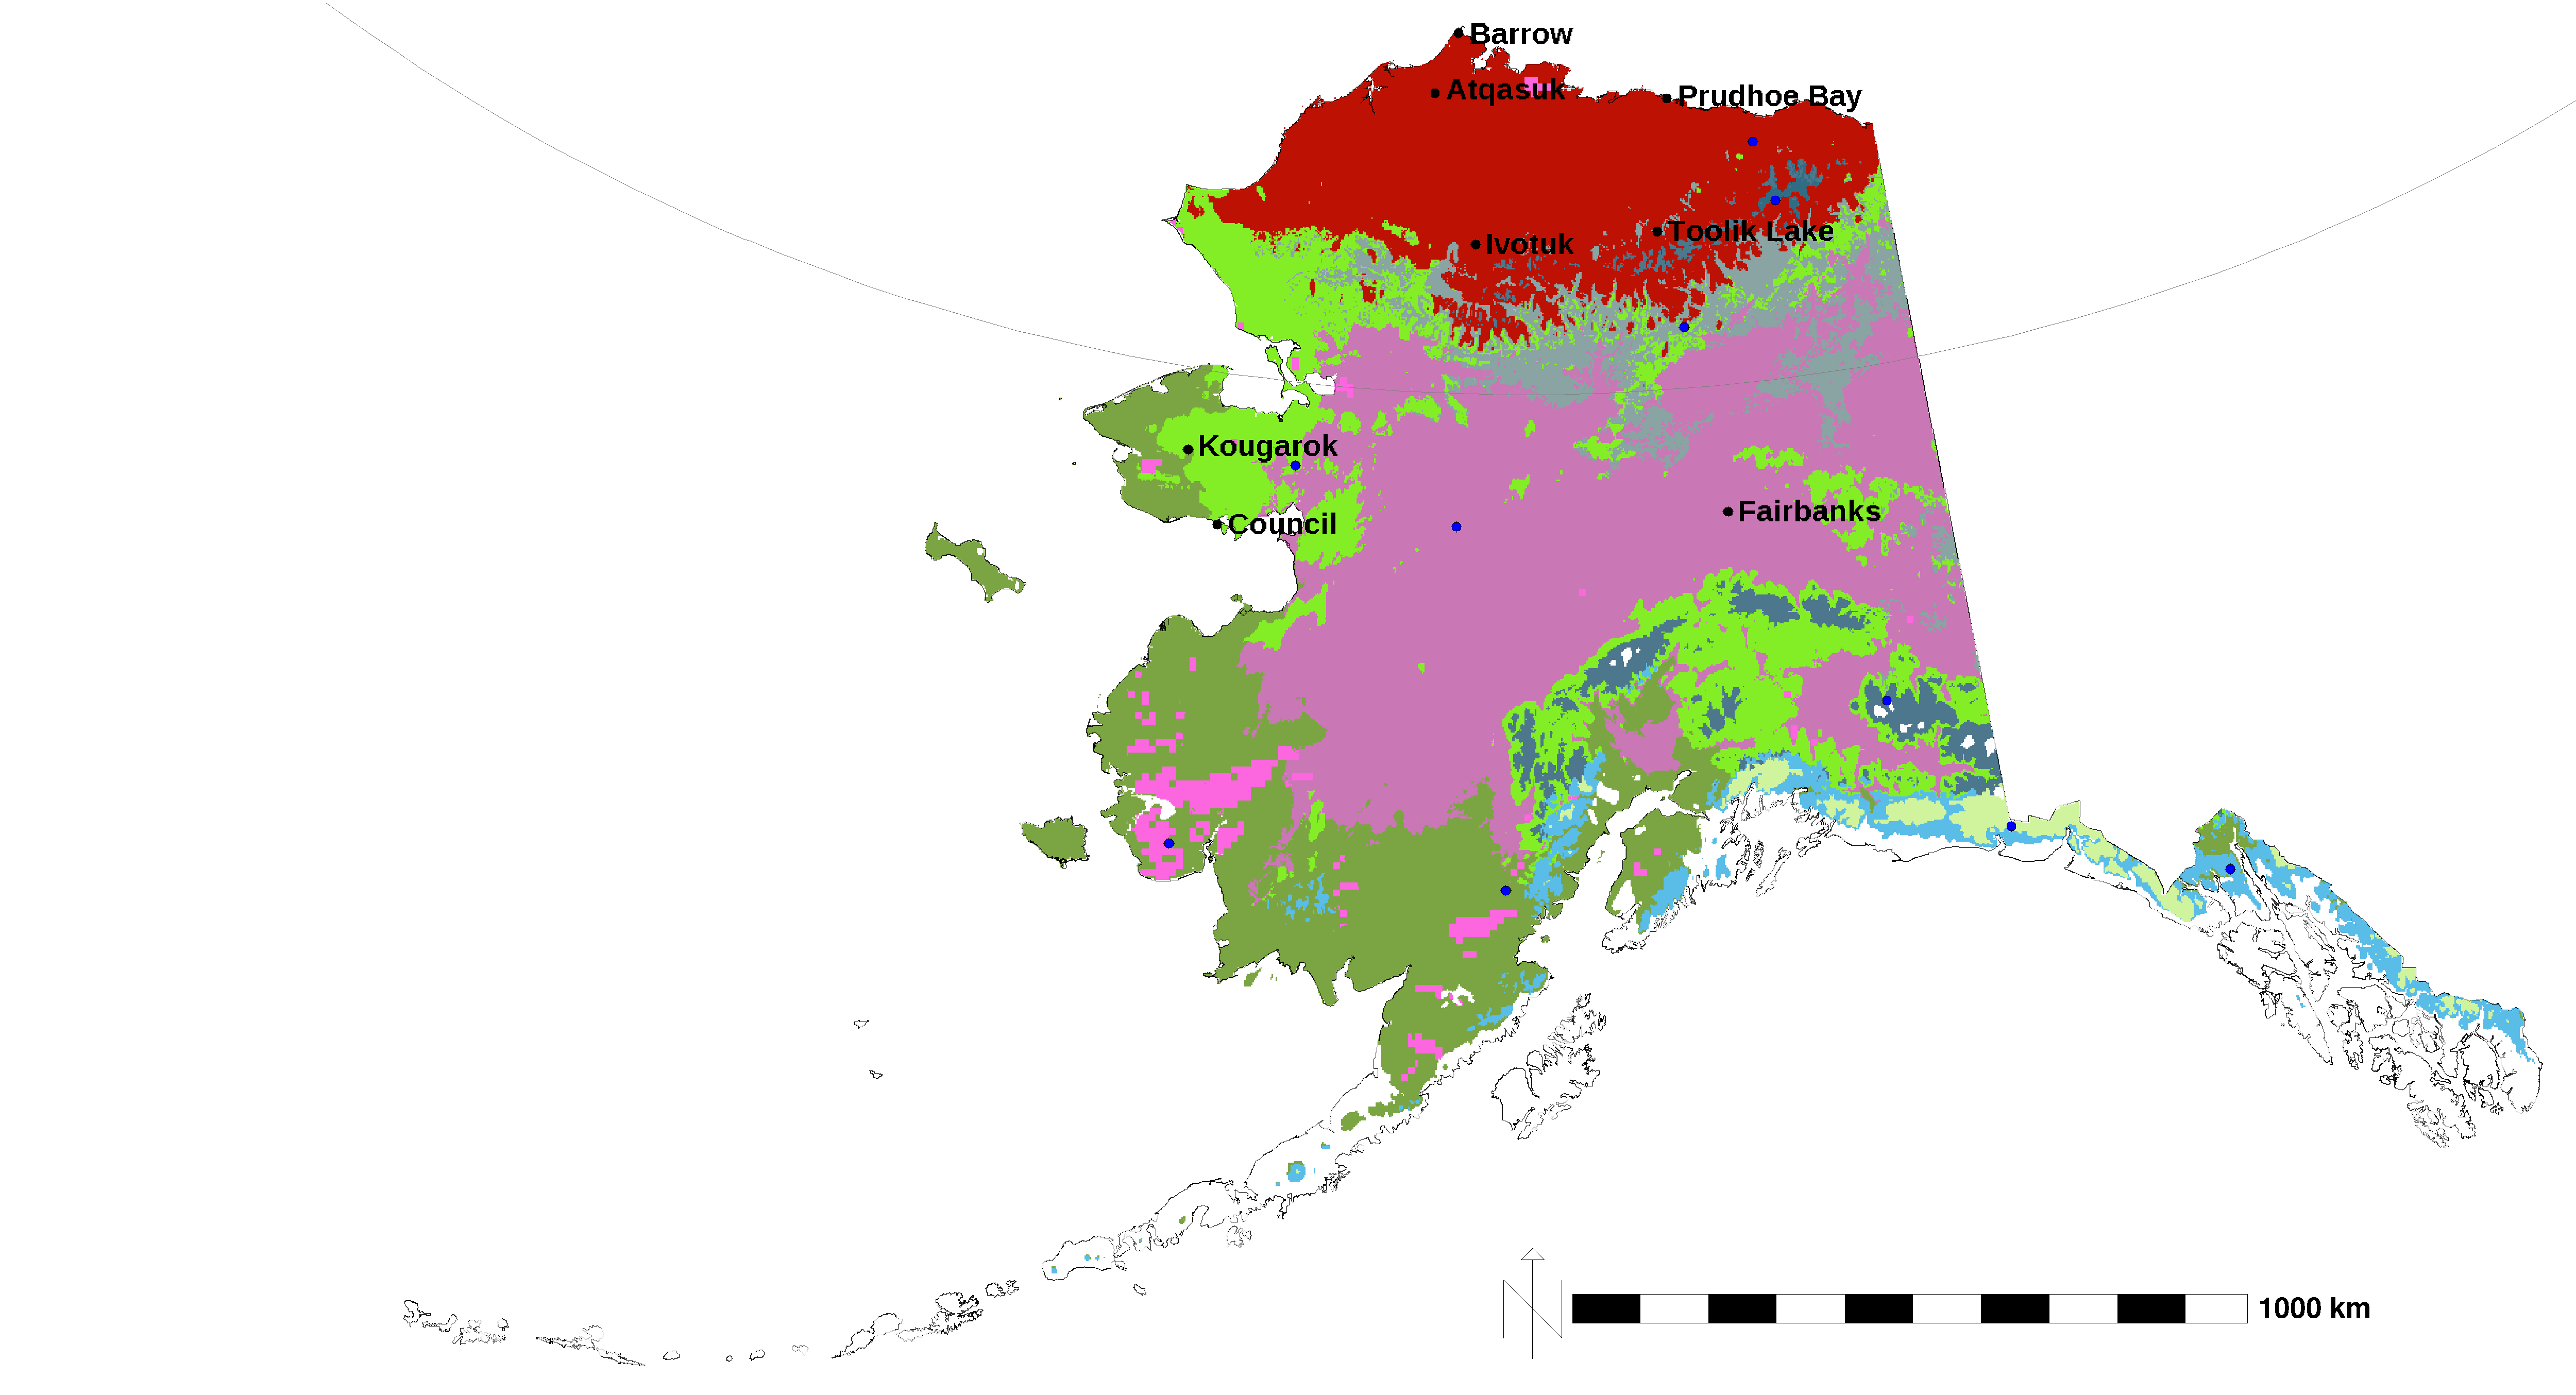
\includegraphics[width=\textwidth]{ngee_figures/alaska_dem_Feb2012_10_2090-2099_barscale}
  \end{center}
  %\caption{Cluster analysis.}
  \label{fig:alaska_2090_2099_10}
 \end{figure}
 \vskip-0.10in
 \vbox{\scriptsize\hfill\citep{Hoffman_LandscapeEcol_20131001}}
\smallskip
Each ecoregion is a different random color. Blue filled circles mark
locations most representative of mean conditions of each region.
\end{frame}
%%%%%%%%%%%%%%%%%%%%%%%%%%%%%%%%%%%%%%%%%%%%%%%%%%%%%%%%%%%%%%%%%%%%%%%%%%%%%%%

%%%%%%%%%%%%%%%%%%%%%%%%%%%%%%%%%%%%%%%%%%%%%%%%%%%%%%%%%%%%%%%%%%%%%%%%%%%%%%%
\begin{frame}
 \frametitle{10 Alaska Ecoregions, Present and Future}
 \vskip-0.15in
 \setlength{\tabcolsep}{0pt}
 \begin{figure}
   \begin{tabular}{cc}
   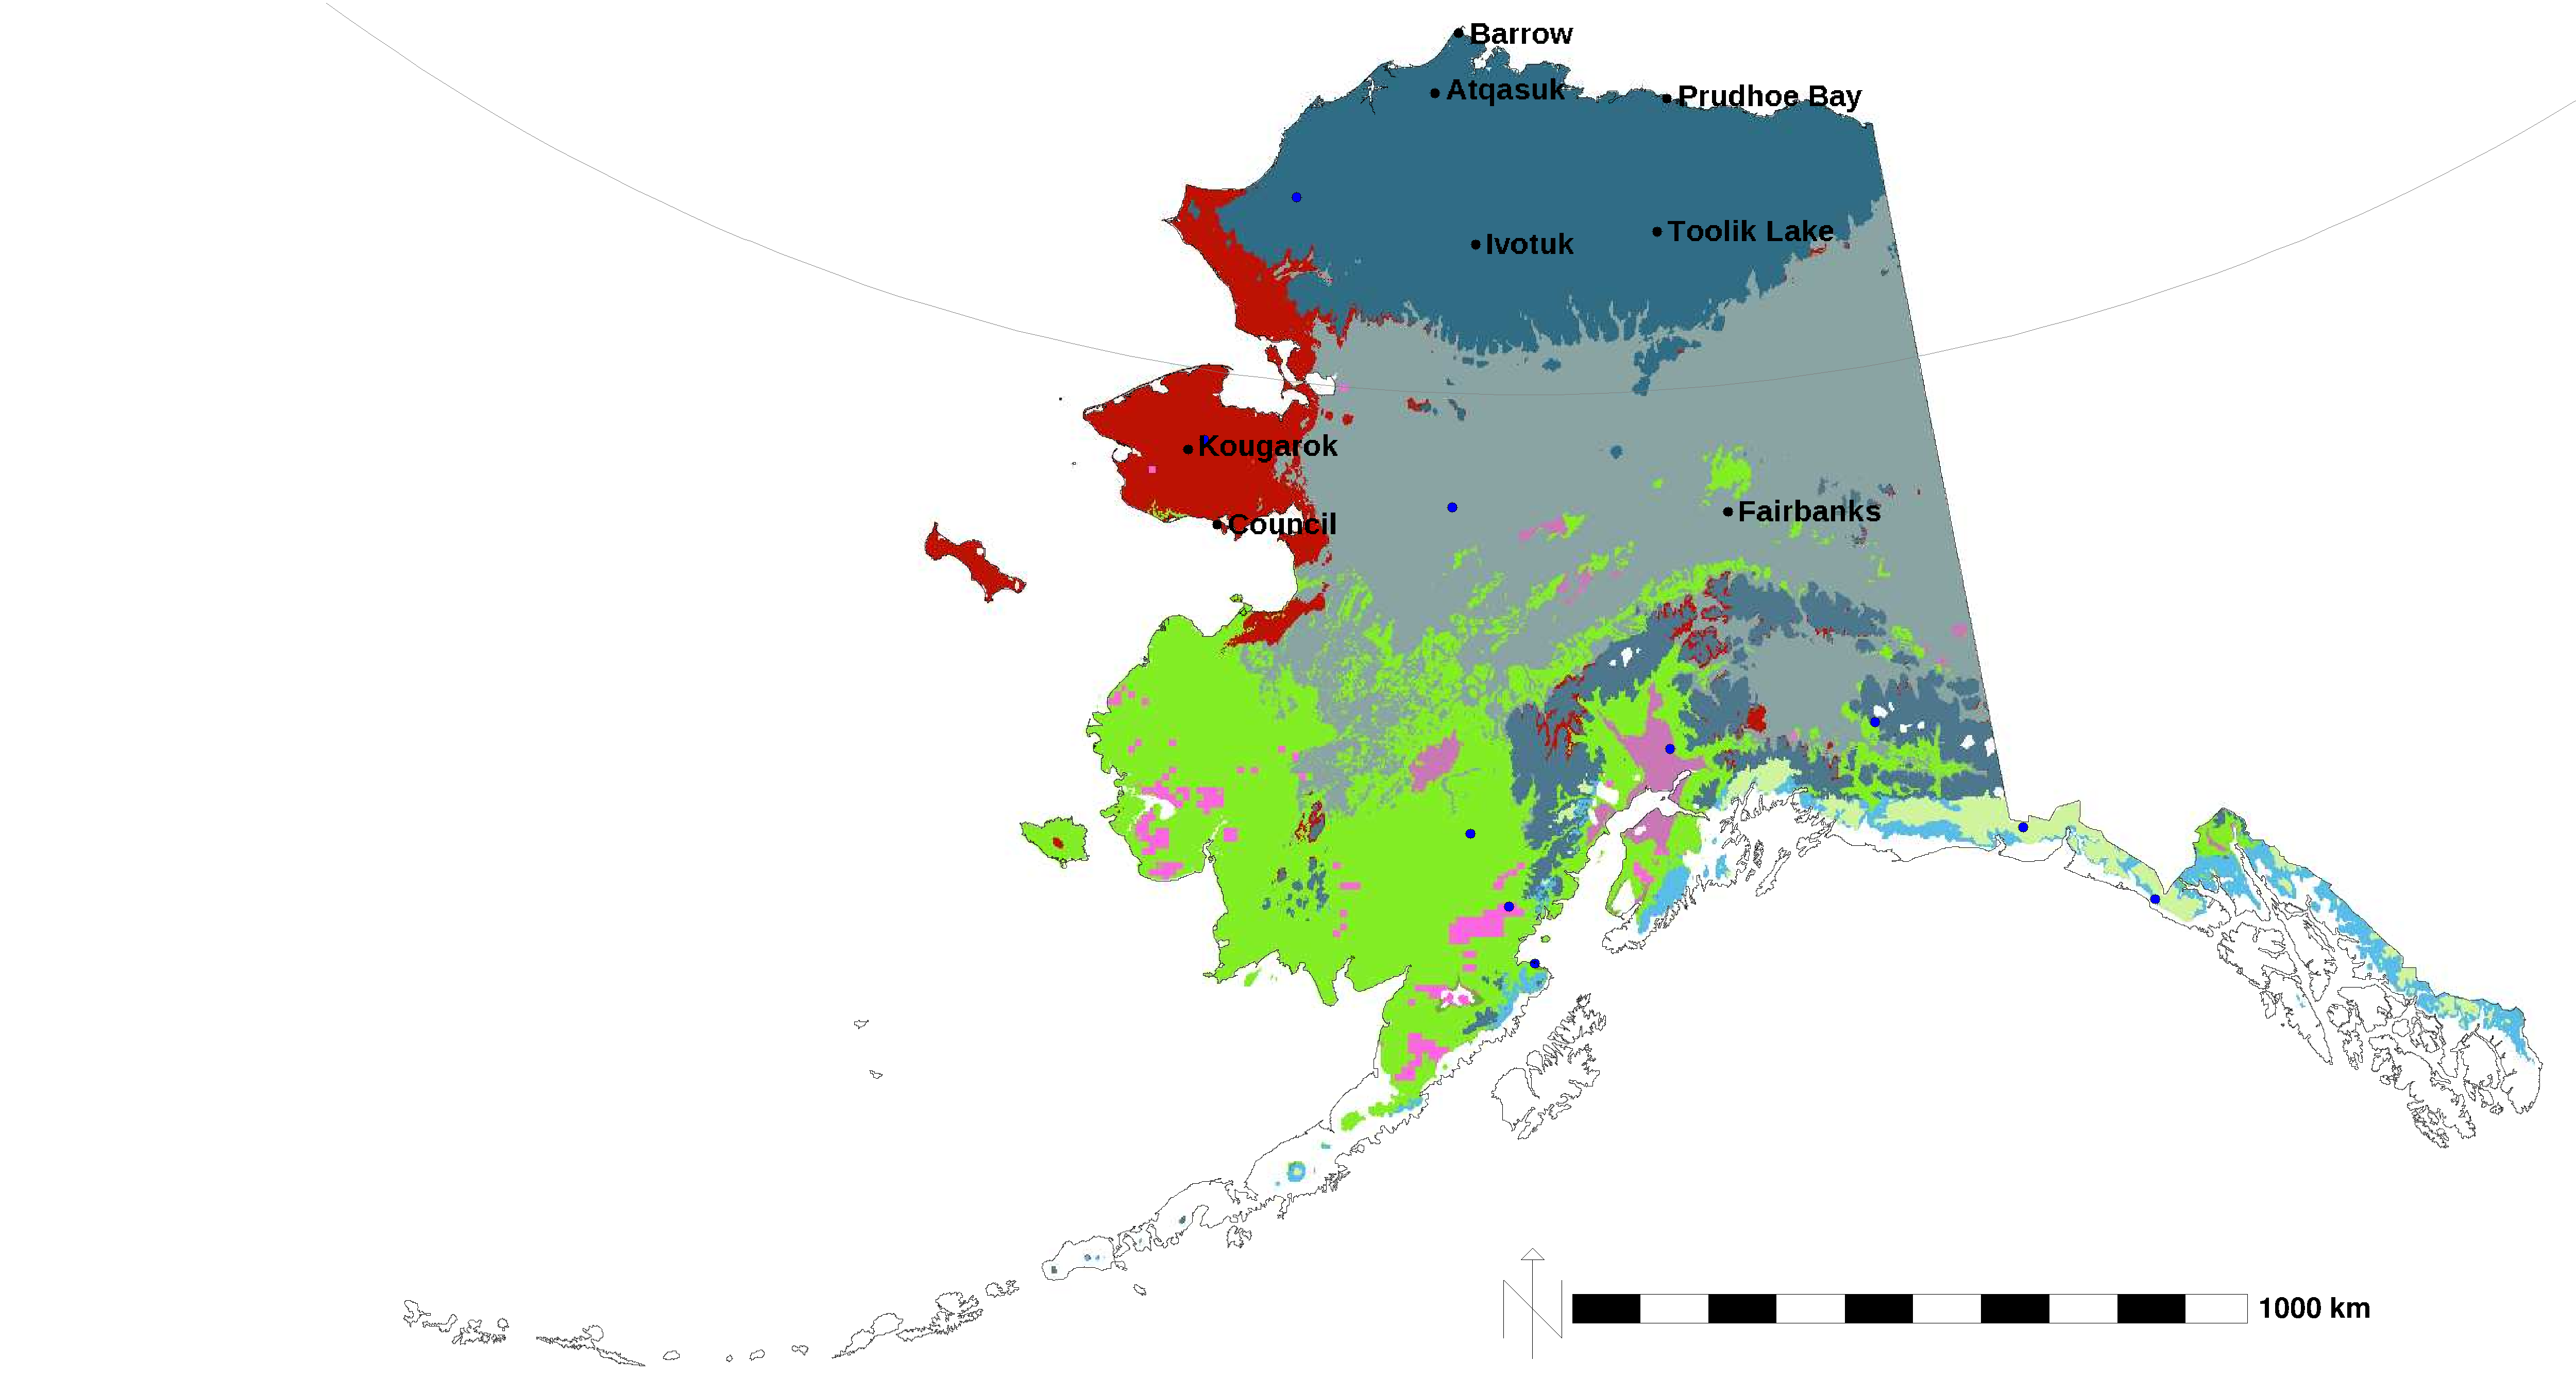
\includegraphics[width=0.50\textwidth]{ngee_figures/alaska_dem_Feb2012_10_2000-2009_barscale} &
   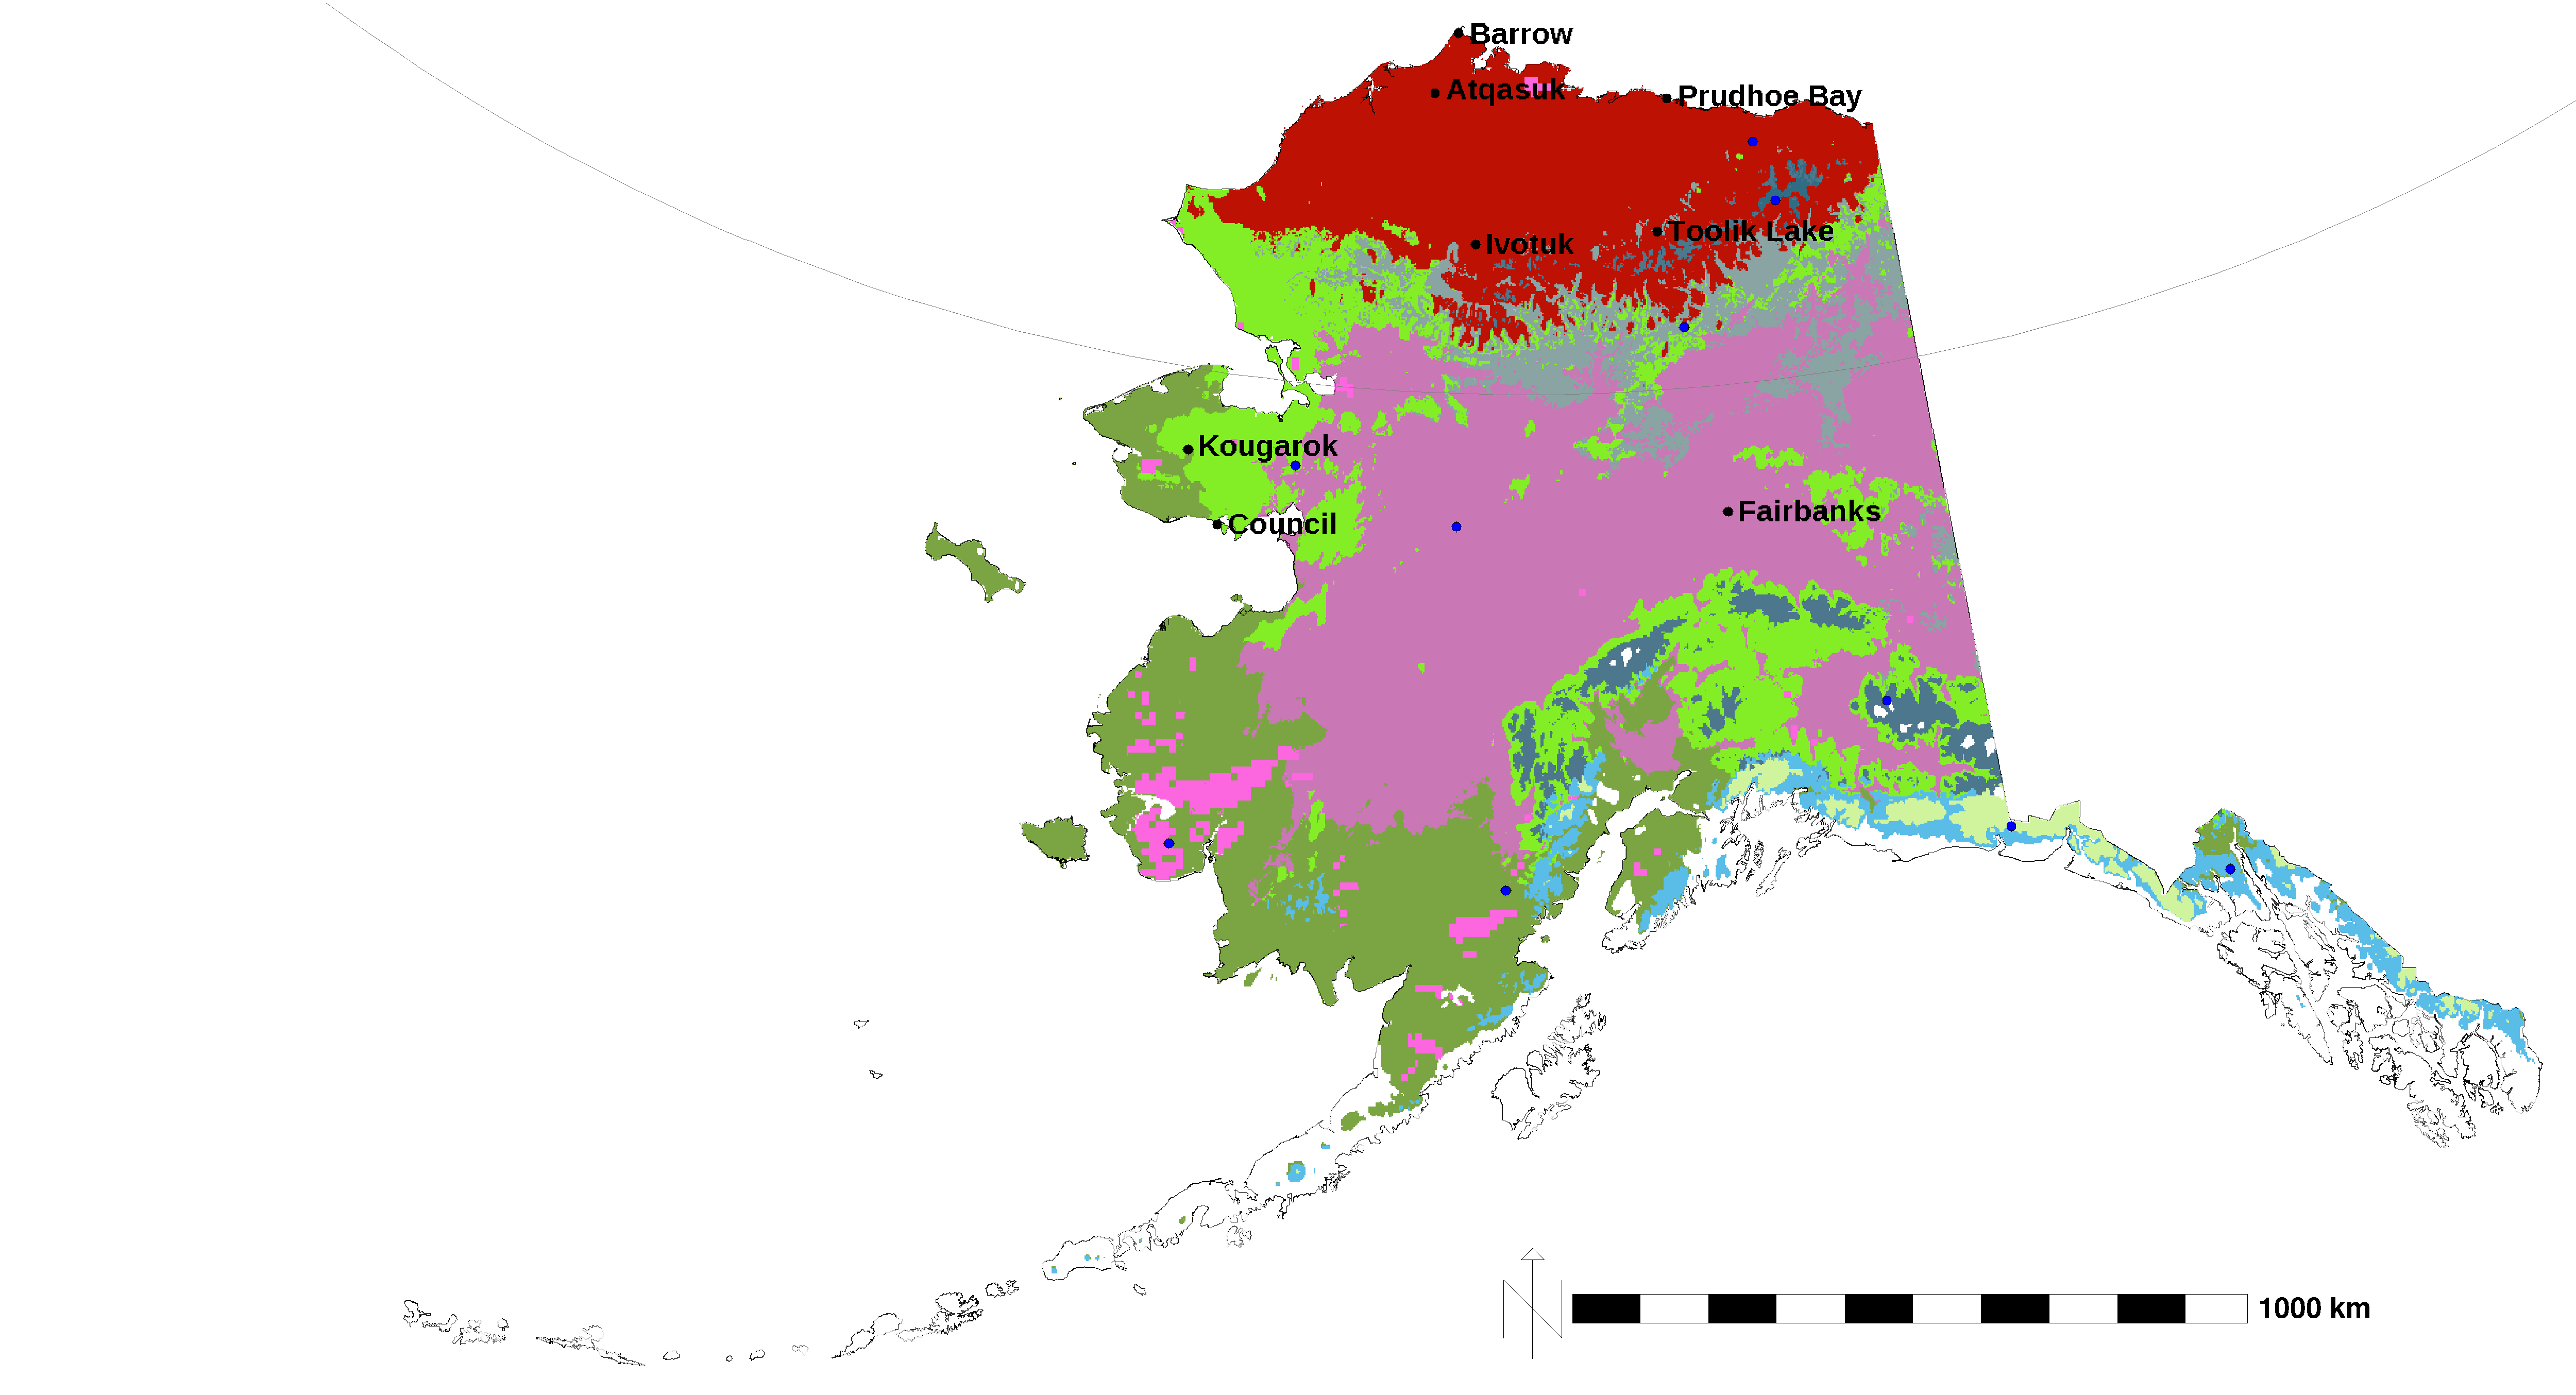
\includegraphics[width=0.50\textwidth]{ngee_figures/alaska_dem_Feb2012_10_2090-2099_barscale} \\
   2000--2009 & 2090--2099 \\
   \end{tabular}
  \vbox{\scriptsize\hfill\citep{Hoffman_LandscapeEcol_20131001}}
  %\caption{Cluster analysis.}
  \label{fig:alaska_both_10}
 \end{figure}
 \vskip-0.15in
\emph{Since the random colors are the same in both maps, a change in color
represents an environmental change between the present and the future.}\\

At this level of division, the conditions in the large boreal forest
become compressed onto the Brooks Range and the conditions on
the Seward Peninsula ``migrate'' to the North Slope.

\end{frame}
%%%%%%%%%%%%%%%%%%%%%%%%%%%%%%%%%%%%%%%%%%%%%%%%%%%%%%%%%%%%%%%%%%%%%%%%%%%%%%%

%%%%%%%%%%%%%%%%%%%%%%%%%%%%%%%%%%%%%%%%%%%%%%%%%%%%%%%%%%%%%%%%%%%%%%%%%%%%%%%
\begin{frame}
 \frametitle{20 Alaska Ecoregions, Present and Future}
 \vskip-0.15in
 \setlength{\tabcolsep}{0pt}
 \begin{figure}
   \begin{tabular}{cc}
   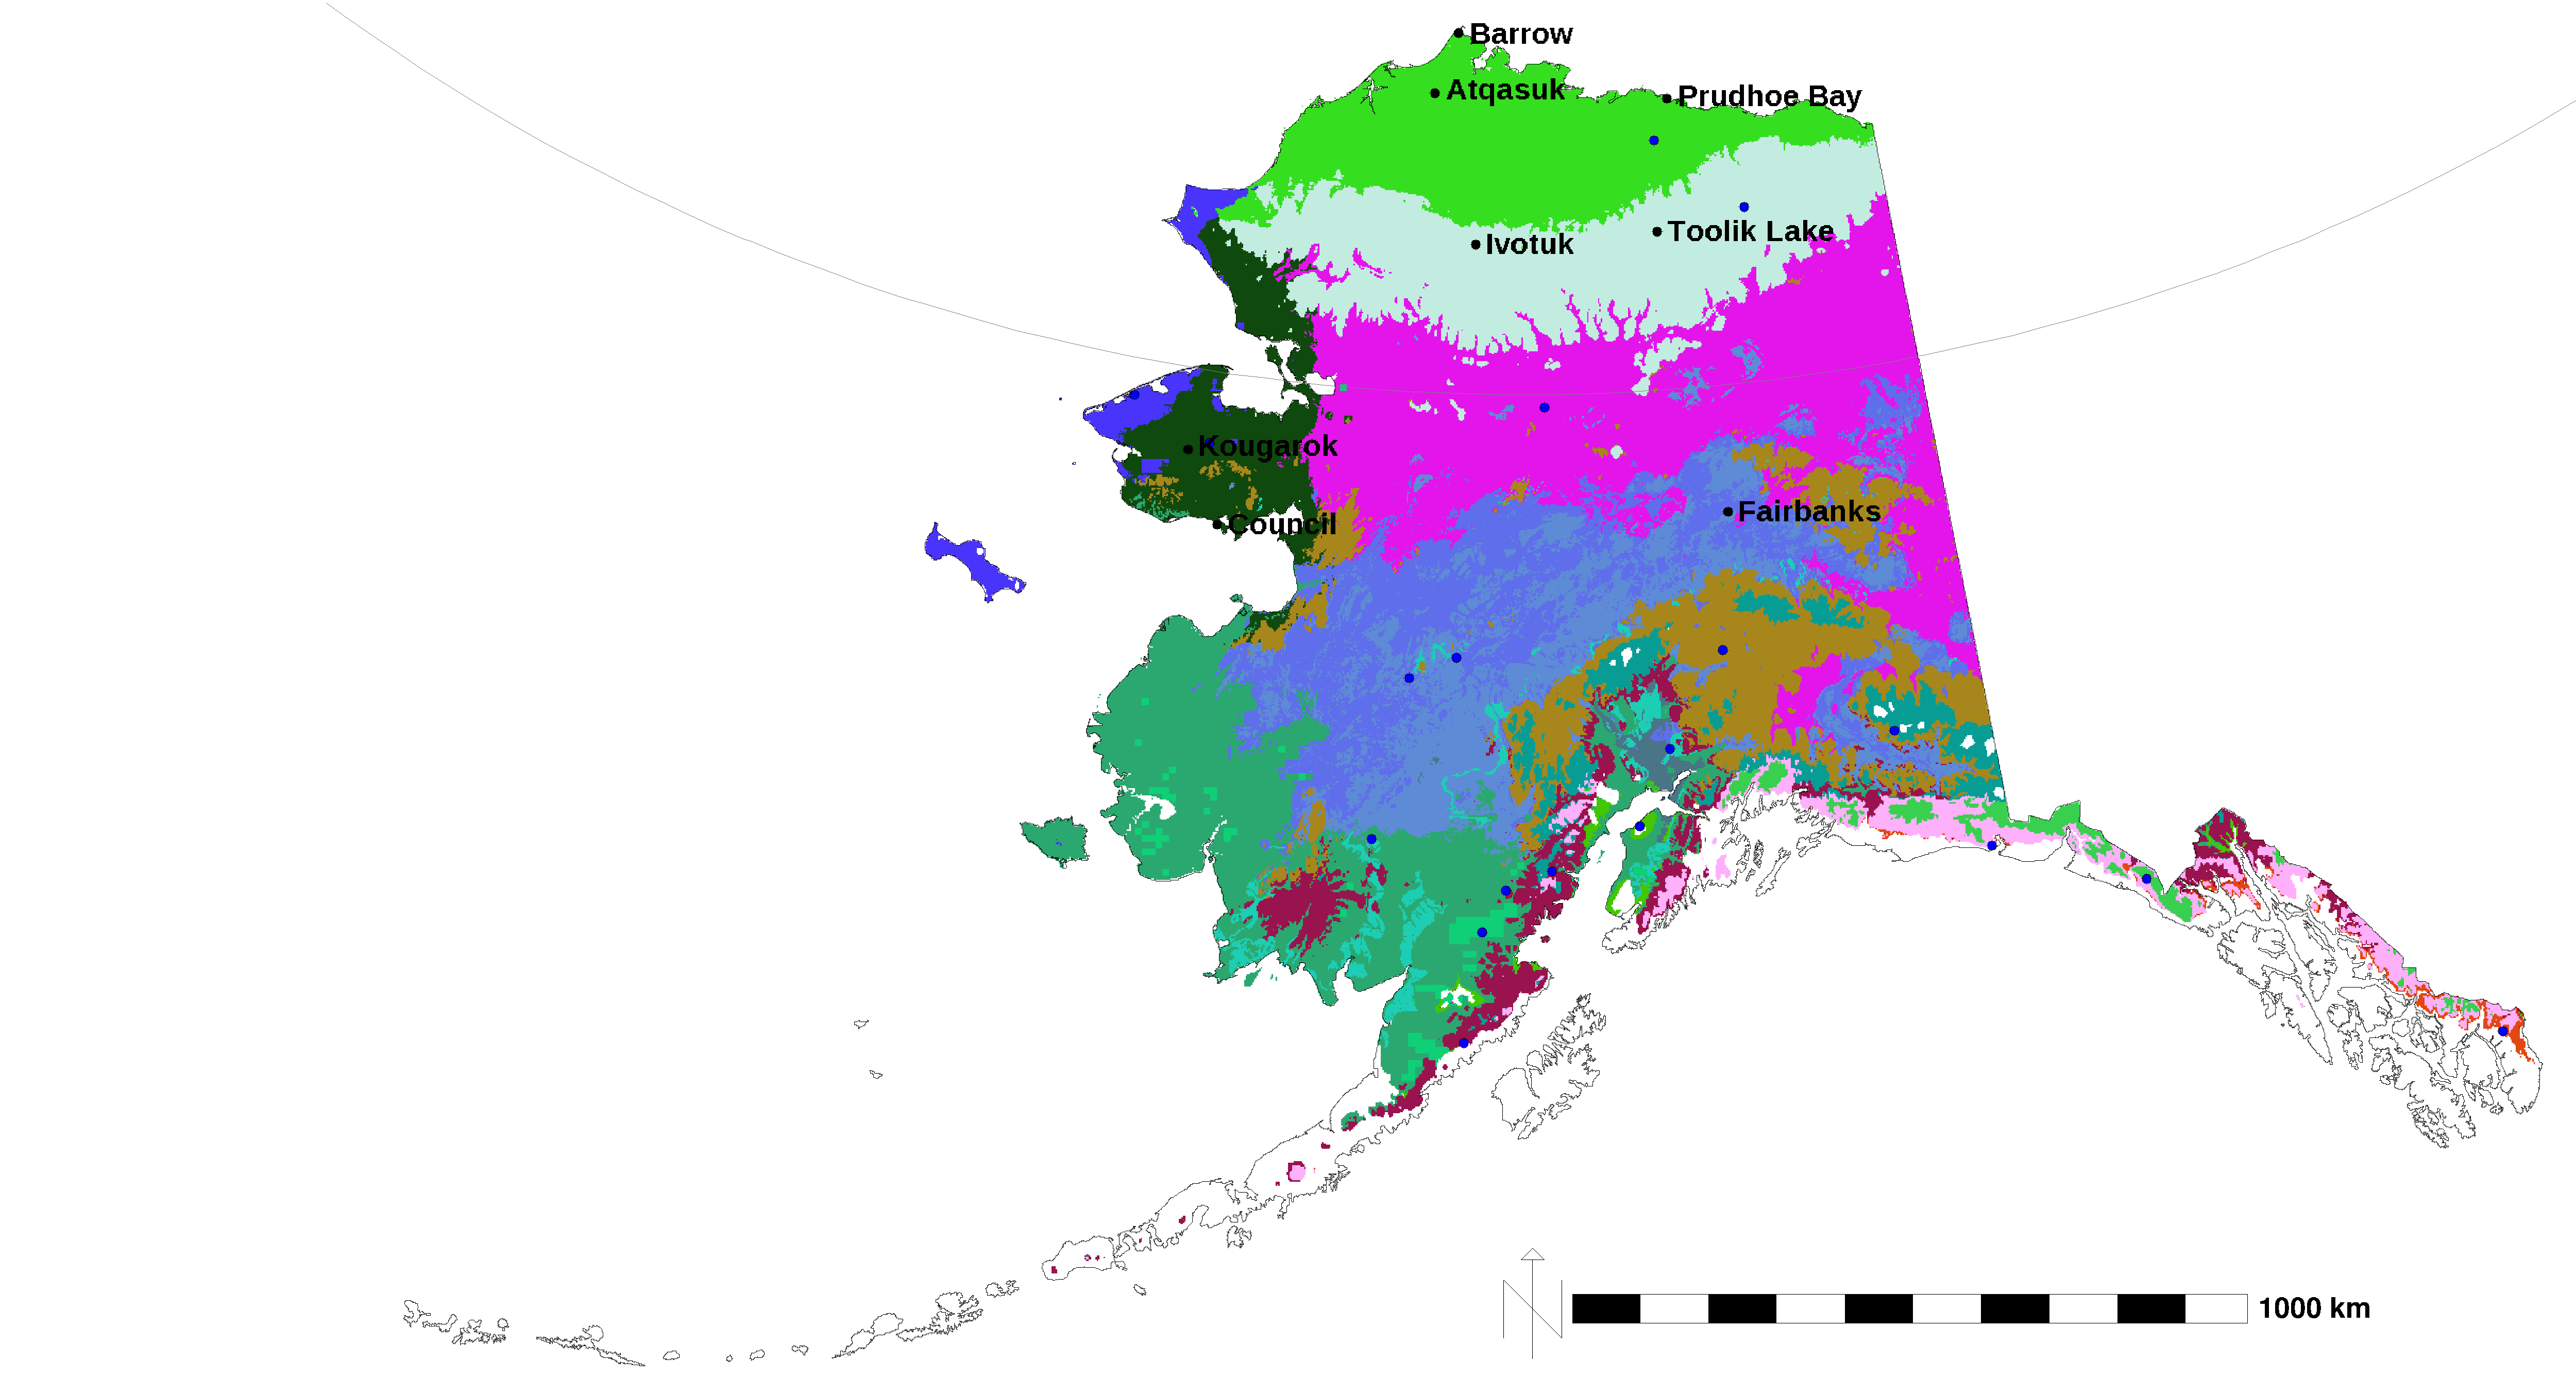
\includegraphics[width=0.50\textwidth]{ngee_figures/alaska_dem_Feb2012_20_2000-2009_barscale} &
   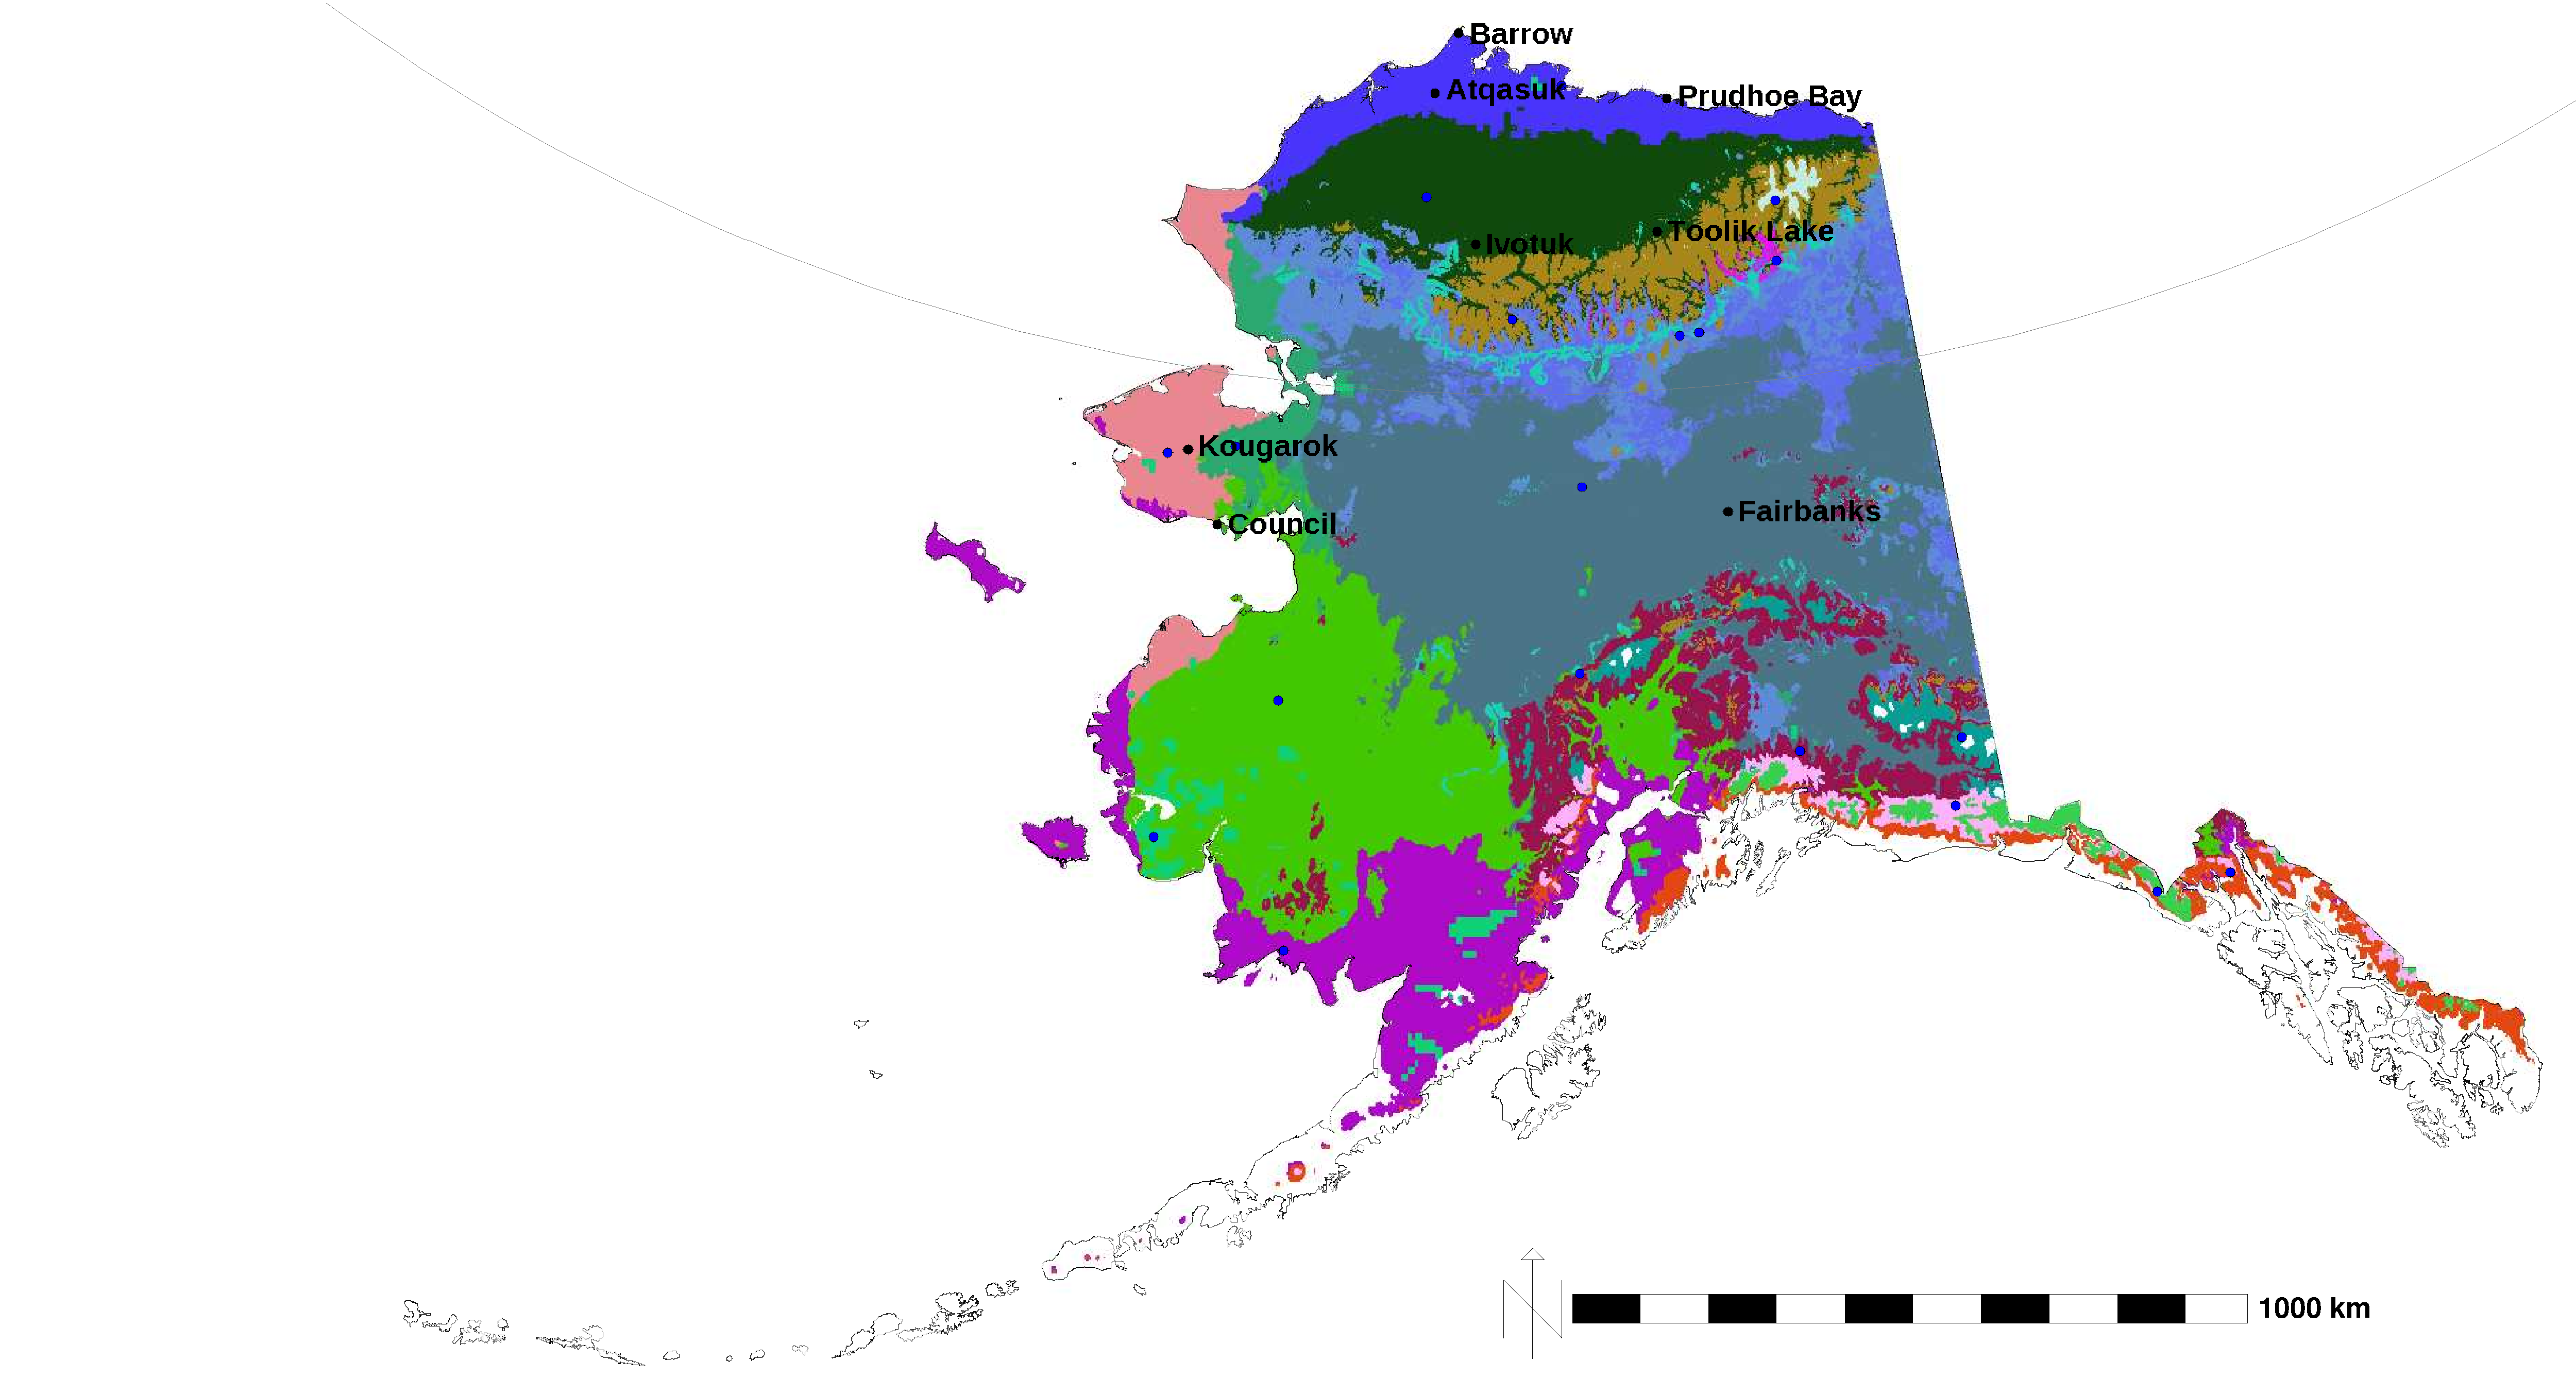
\includegraphics[width=0.50\textwidth]{ngee_figures/alaska_dem_Feb2012_20_2090-2099_barscale} \\
   2000--2009 & 2090--2099 \\
   \end{tabular}
  \vbox{\scriptsize\hfill\citep{Hoffman_LandscapeEcol_20131001}}
  %\caption{Cluster analysis.}
  \label{fig:alaska_both_20}
 \end{figure}
 \vskip-0.15in
\emph{Since the random colors are the same in both maps, a change in color
represents an environmental change between the present and the future.}

At this level of division, the two primary regions of the Seward
Peninsula and that of the northern boreal forest replace the two
regions on the North Slope almost entirely.

\end{frame}
%%%%%%%%%%%%%%%%%%%%%%%%%%%%%%%%%%%%%%%%%%%%%%%%%%%%%%%%%%%%%%%%%%%%%%%%%%%%%%%

%%%%%%%%%%%%%%%%%%%%%%%%%%%%%%%%%%%%%%%%%%%%%%%%%%%%%%%%%%%%%%%%%%%%%%%%%%%%%%%
\begin{frame}
 \frametitle{50 and 100 Alaska Ecoregions, Present}
 \vskip-0.15in
 \setlength{\tabcolsep}{0pt}
 \begin{figure}
   \begin{tabular}{cc}
   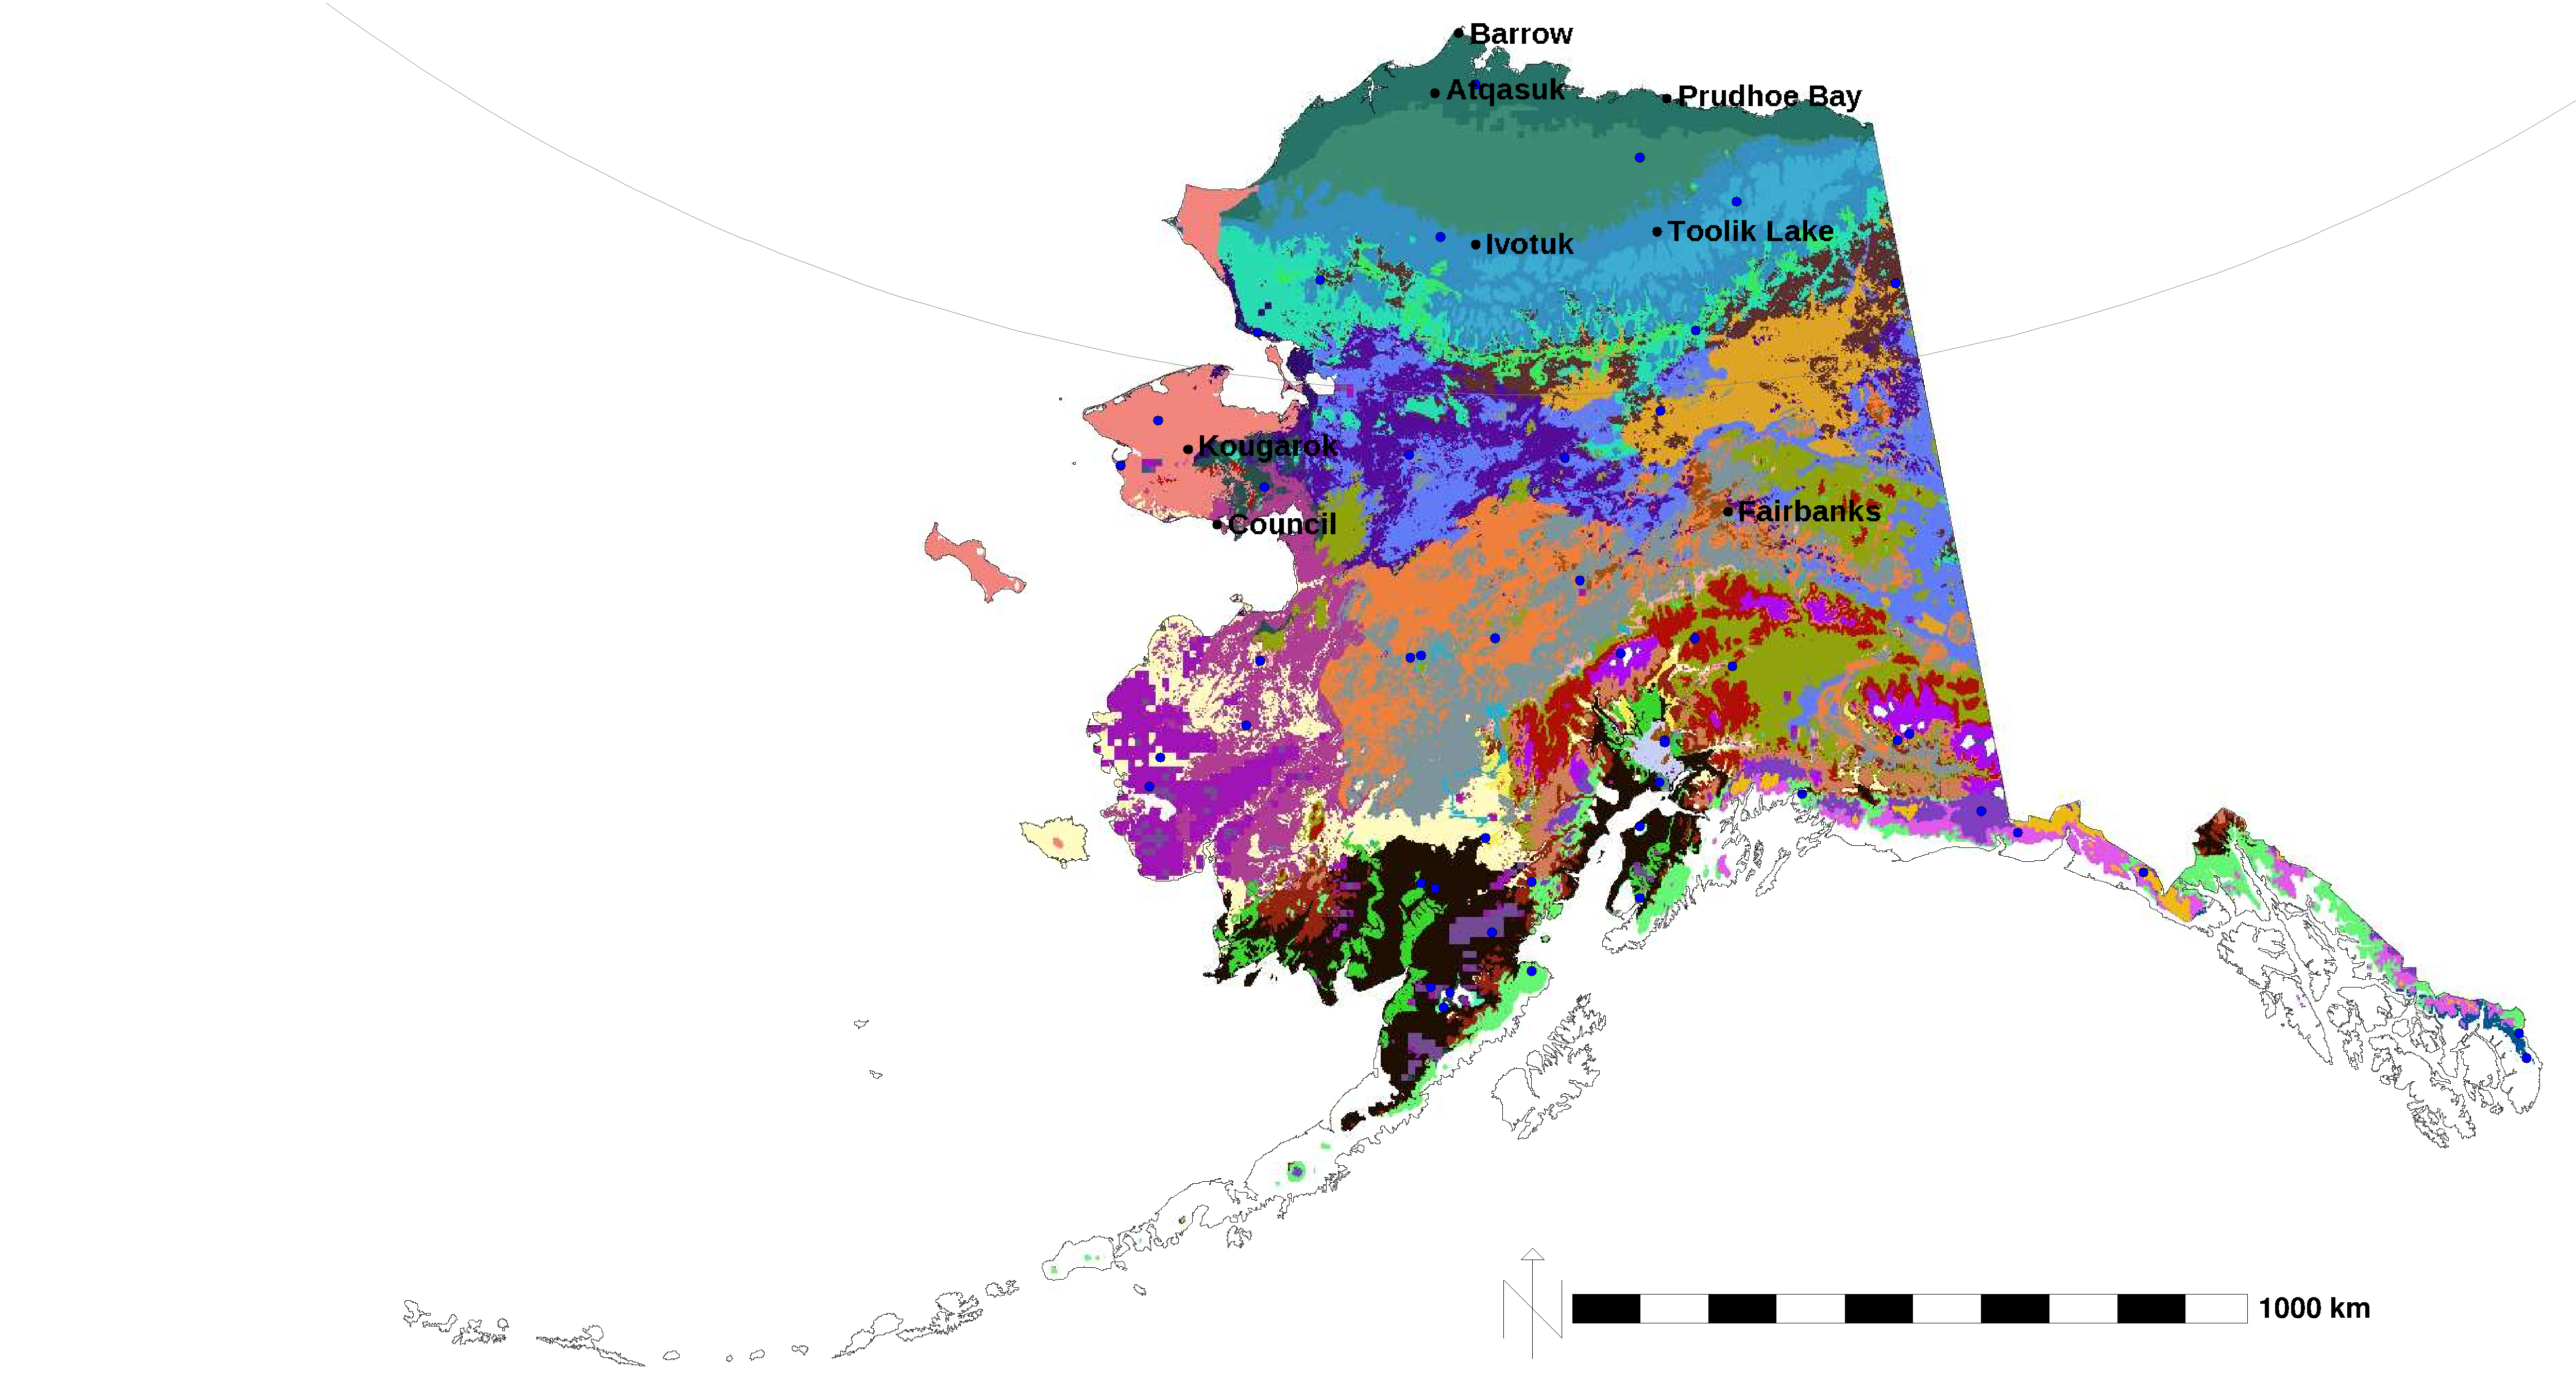
\includegraphics[width=0.50\textwidth]{ngee_figures/alaska_dem_Feb2012_50_2000-2009_barscale} &
   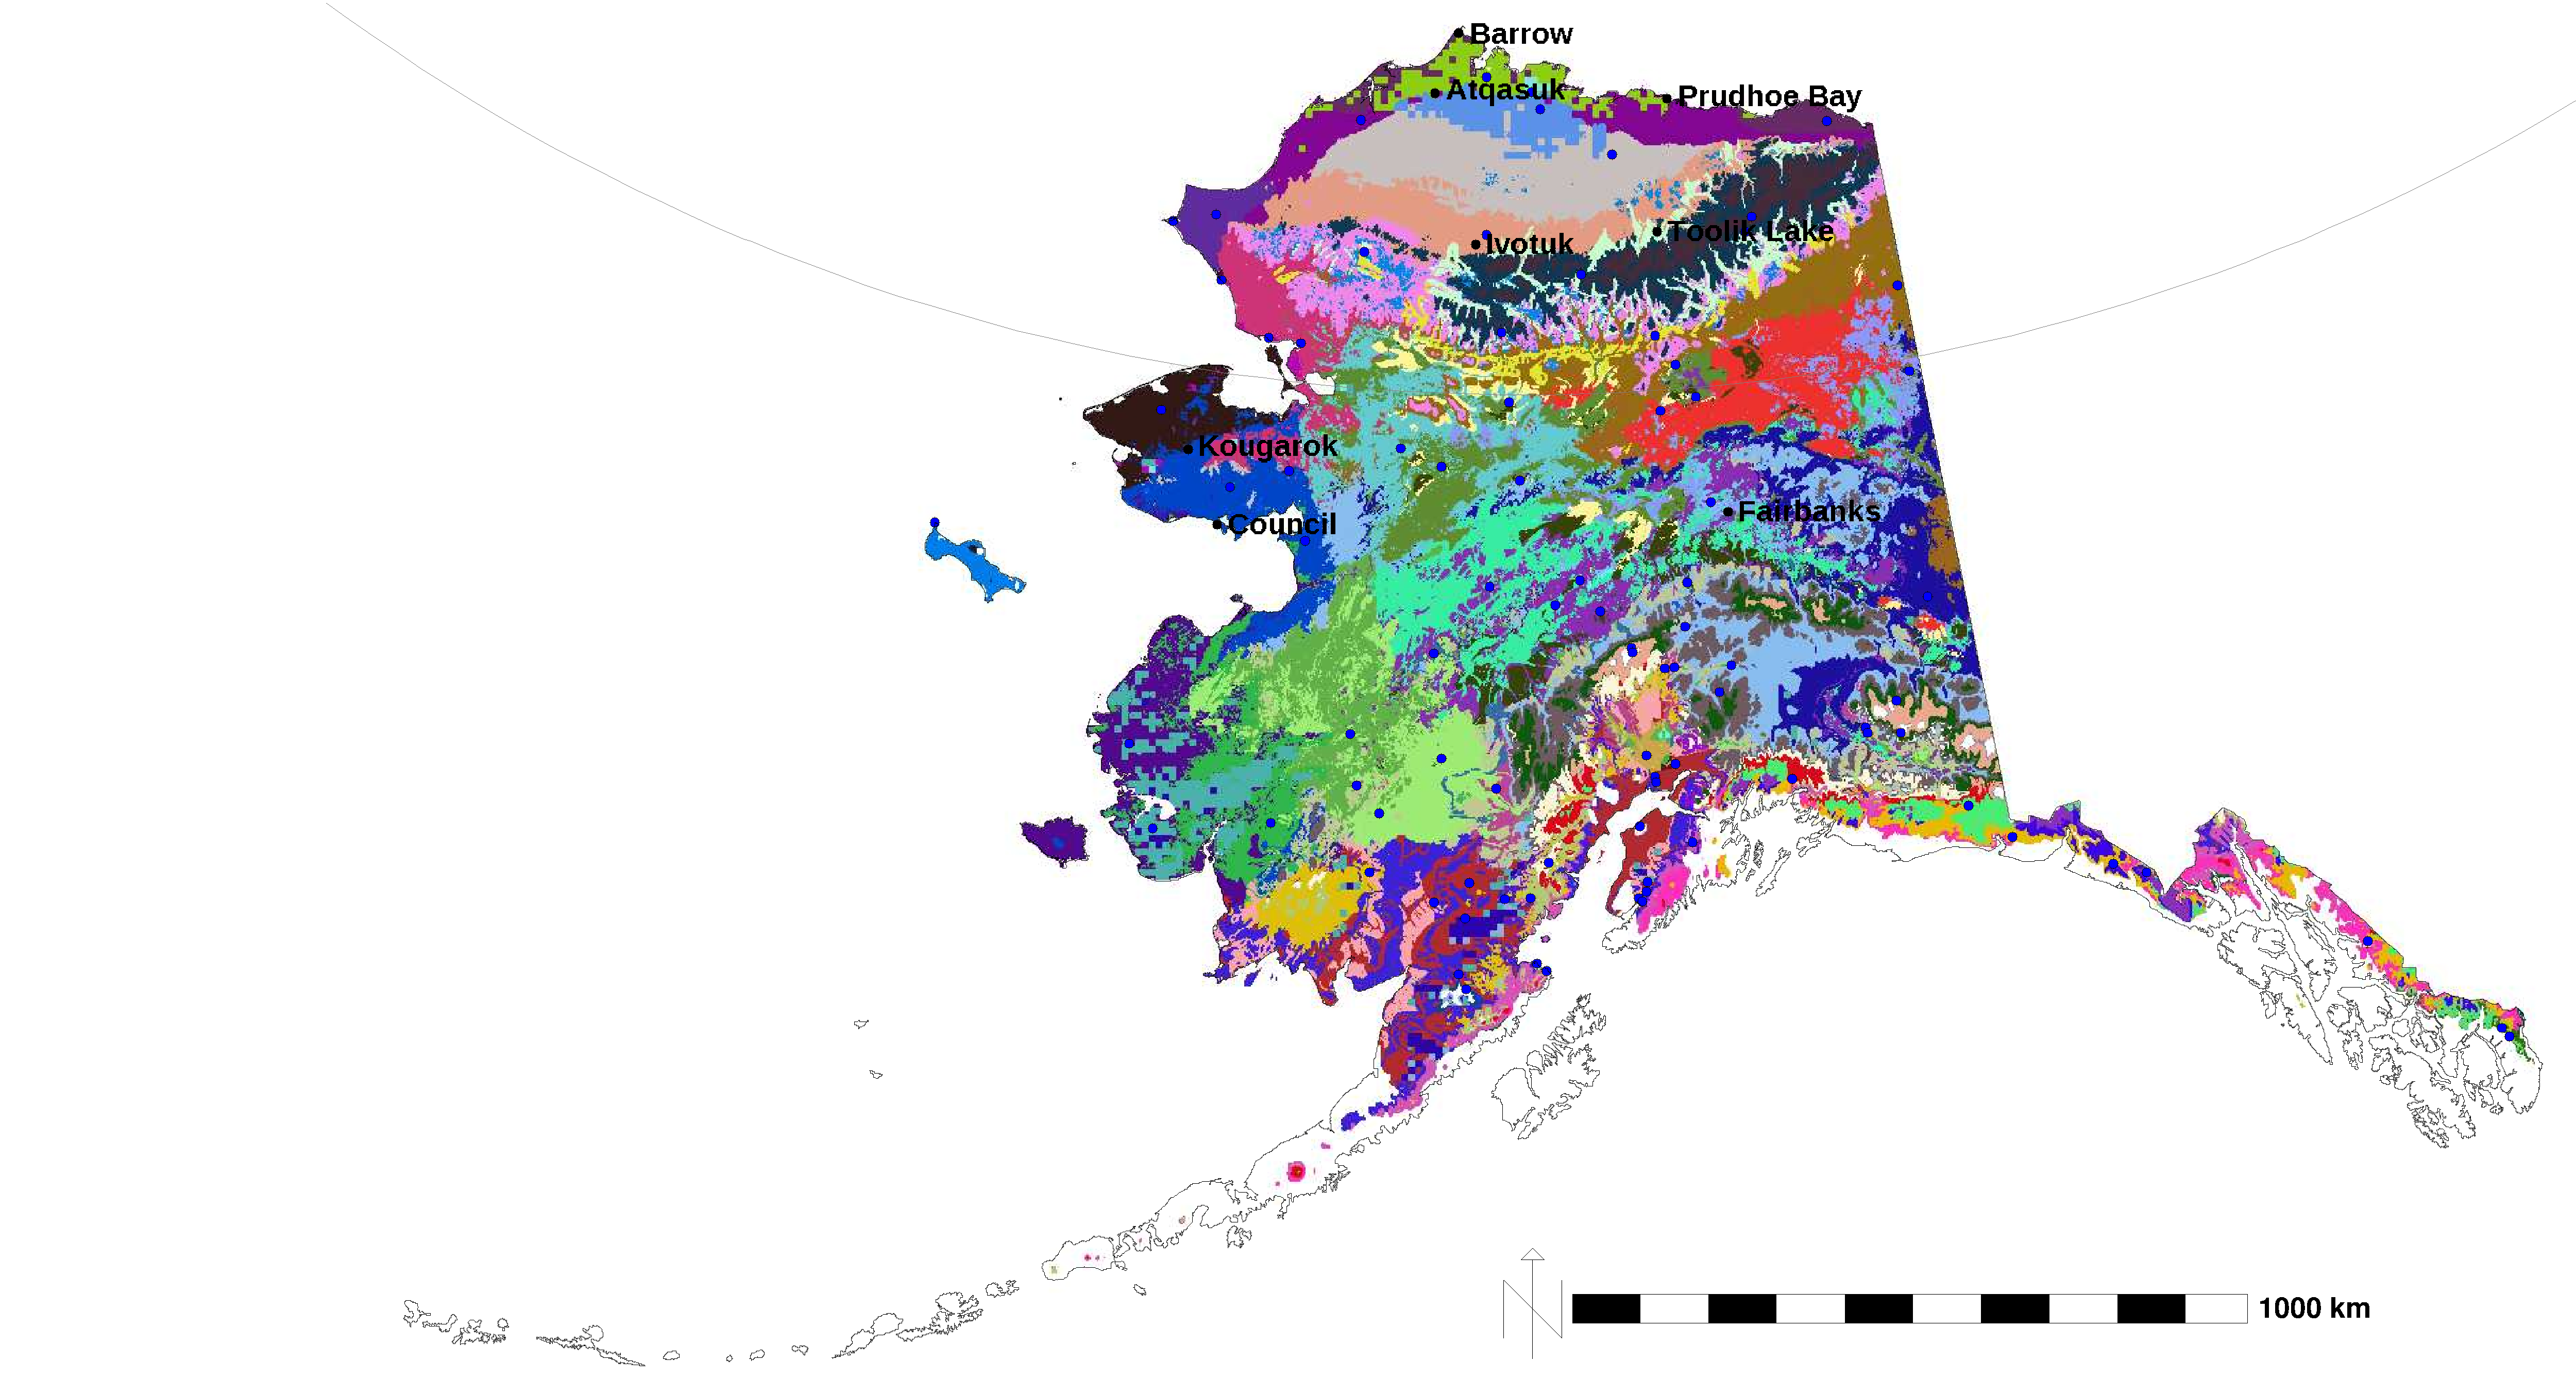
\includegraphics[width=0.50\textwidth]{ngee_figures/alaska_dem_Feb2012_100_2000-2009_barscale} \\
   $k=50$, 2000--2009 & $k=100$, 2000--2009 \\
   \end{tabular}
  \vbox{\scriptsize\hfill\citep{Hoffman_LandscapeEcol_20131001}}
  %\caption{Cluster analysis.}
  \label{fig:alaska_present_50_100}
 \end{figure}
 \vskip-0.15in
\emph{Since the random colors are the same in both maps, a change in color
represents an environmental change between the present and the future.}\\

At high levels of division, some regions vanish between the present
and future while other region representing new combinations of
environmental conditions come into existence.

\end{frame}
%%%%%%%%%%%%%%%%%%%%%%%%%%%%%%%%%%%%%%%%%%%%%%%%%%%%%%%%%%%%%%%%%%%%%%%%%%%%%%%

%%%%%%%%%%%%%%%%%%%%%%%%%%%%%%%%%%%%%%%%%%%%%%%%%%%%%%%%%%%%%%%%%%%%%%%%%%%
% Hierarchical ecoregions
%%%%%%%%%%%%%%%%%%%%%%%%%%%%%%%%%%%%%%%%%%%%%%%%%%%%%%%%%%%%%%%%%%%%%%%%%%%
%\begin{frame}
% \frametitle{A Hierarchy of Ecoregions}
% %\vbox{\centering\large\textbf{\color{blue}A Hierarchy of Ecoregions}}
% \vskip-0.15in
%\begin{figure}\scriptsize
%  \subfigure[\scriptsize At $k = 10$, the North Slope is occupied by
%Ecoregion \#3, which corresponds to the Arctic Tundra Level 2 ecological
%group.]{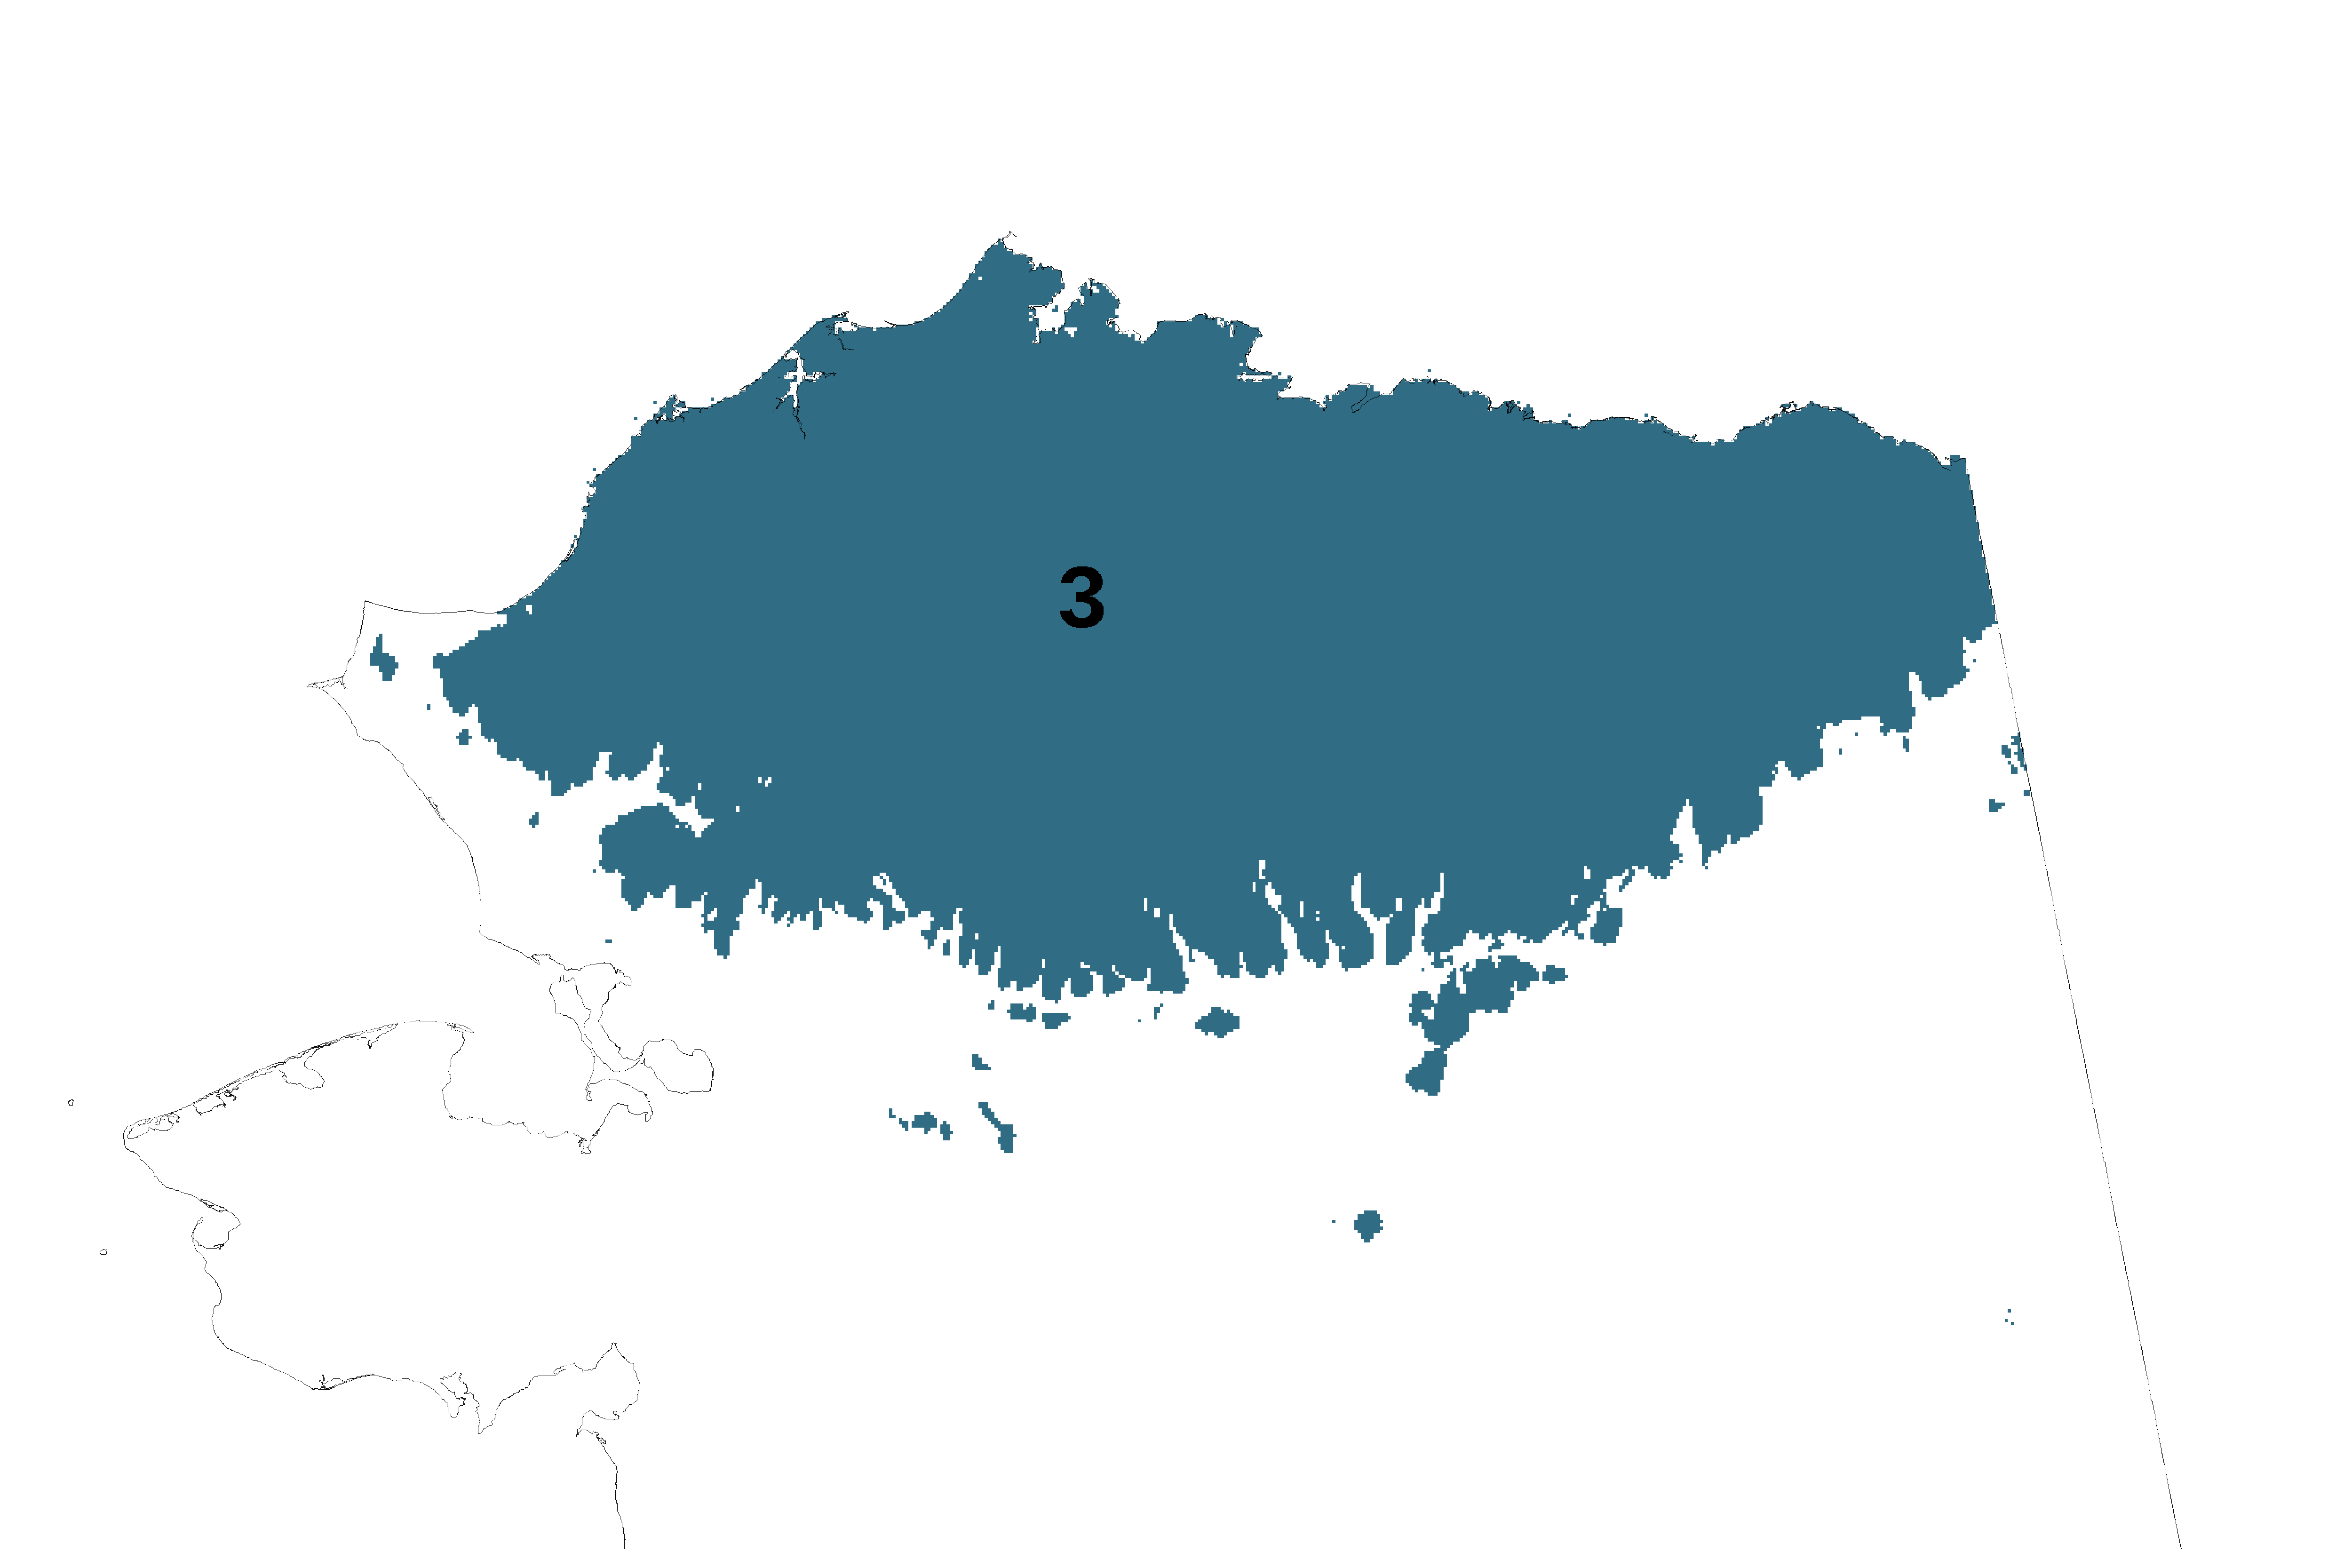
\includegraphics[width=0.315\textwidth]{ngee_figures/arctic_tundra_k10.pdf}\label{fig:k10_NSA}} \hfill
%   \subfigure[\scriptsize At $k = 20$, the North Slope is occupied by 
%Ecoregion \#5, corresponding to the Brooks Range ecoregion; and 
%Ecoregion \#13, corresponding to the Beaufort Coastal Plains
%ecoregion.]{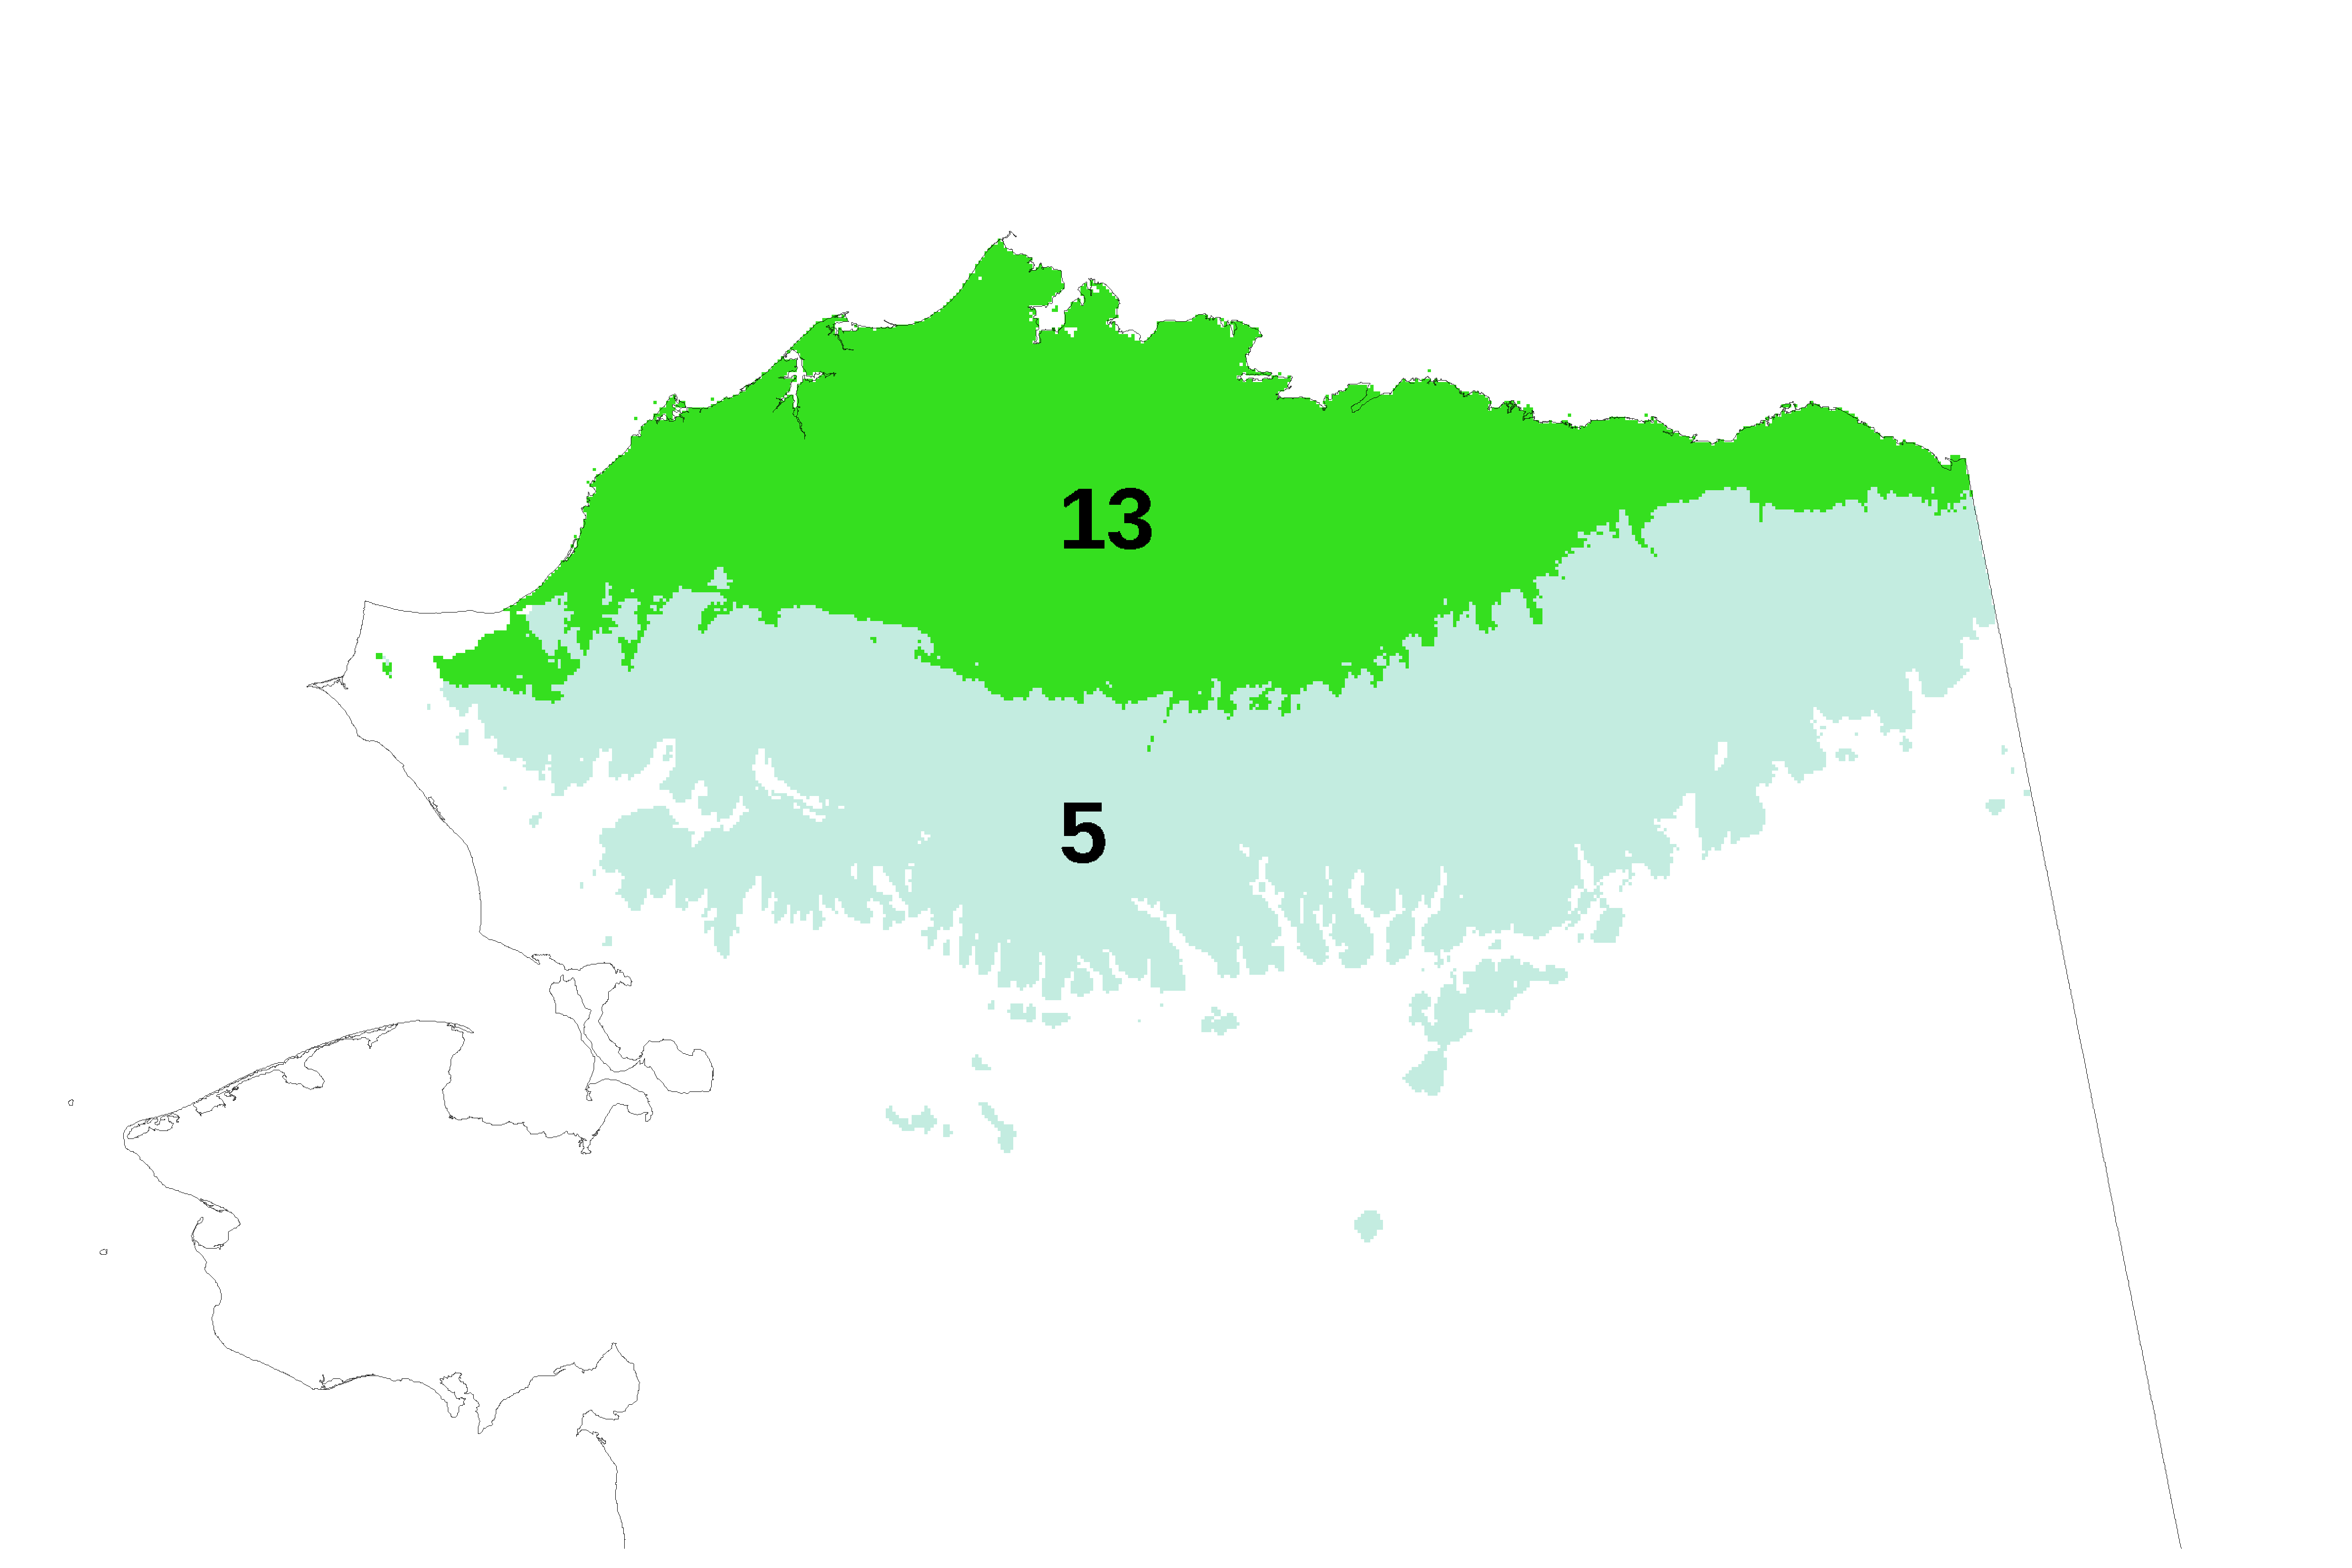
\includegraphics[width=0.315\textwidth]{ngee_figures/arctic_tundra_k20.pdf}\label{fig:k20_NSA}} \hfill
%   \subfigure[\scriptsize At $k = 50$, the North Slope is occupied by 
%Ecoregion \#32, corresponding to the Intermontane Boreal ecological group;
%Ecoregions \#33 and \#34, corresponding to mid- and high-elevation
%of the Brooks Range ecoregion; Ecoregion \#35,
%corresponding to the Brooks Foothills ecoregion; and Ecoregion \#40,
%corresponding to the Beaufort Coastal Plains
%ecoregion.]{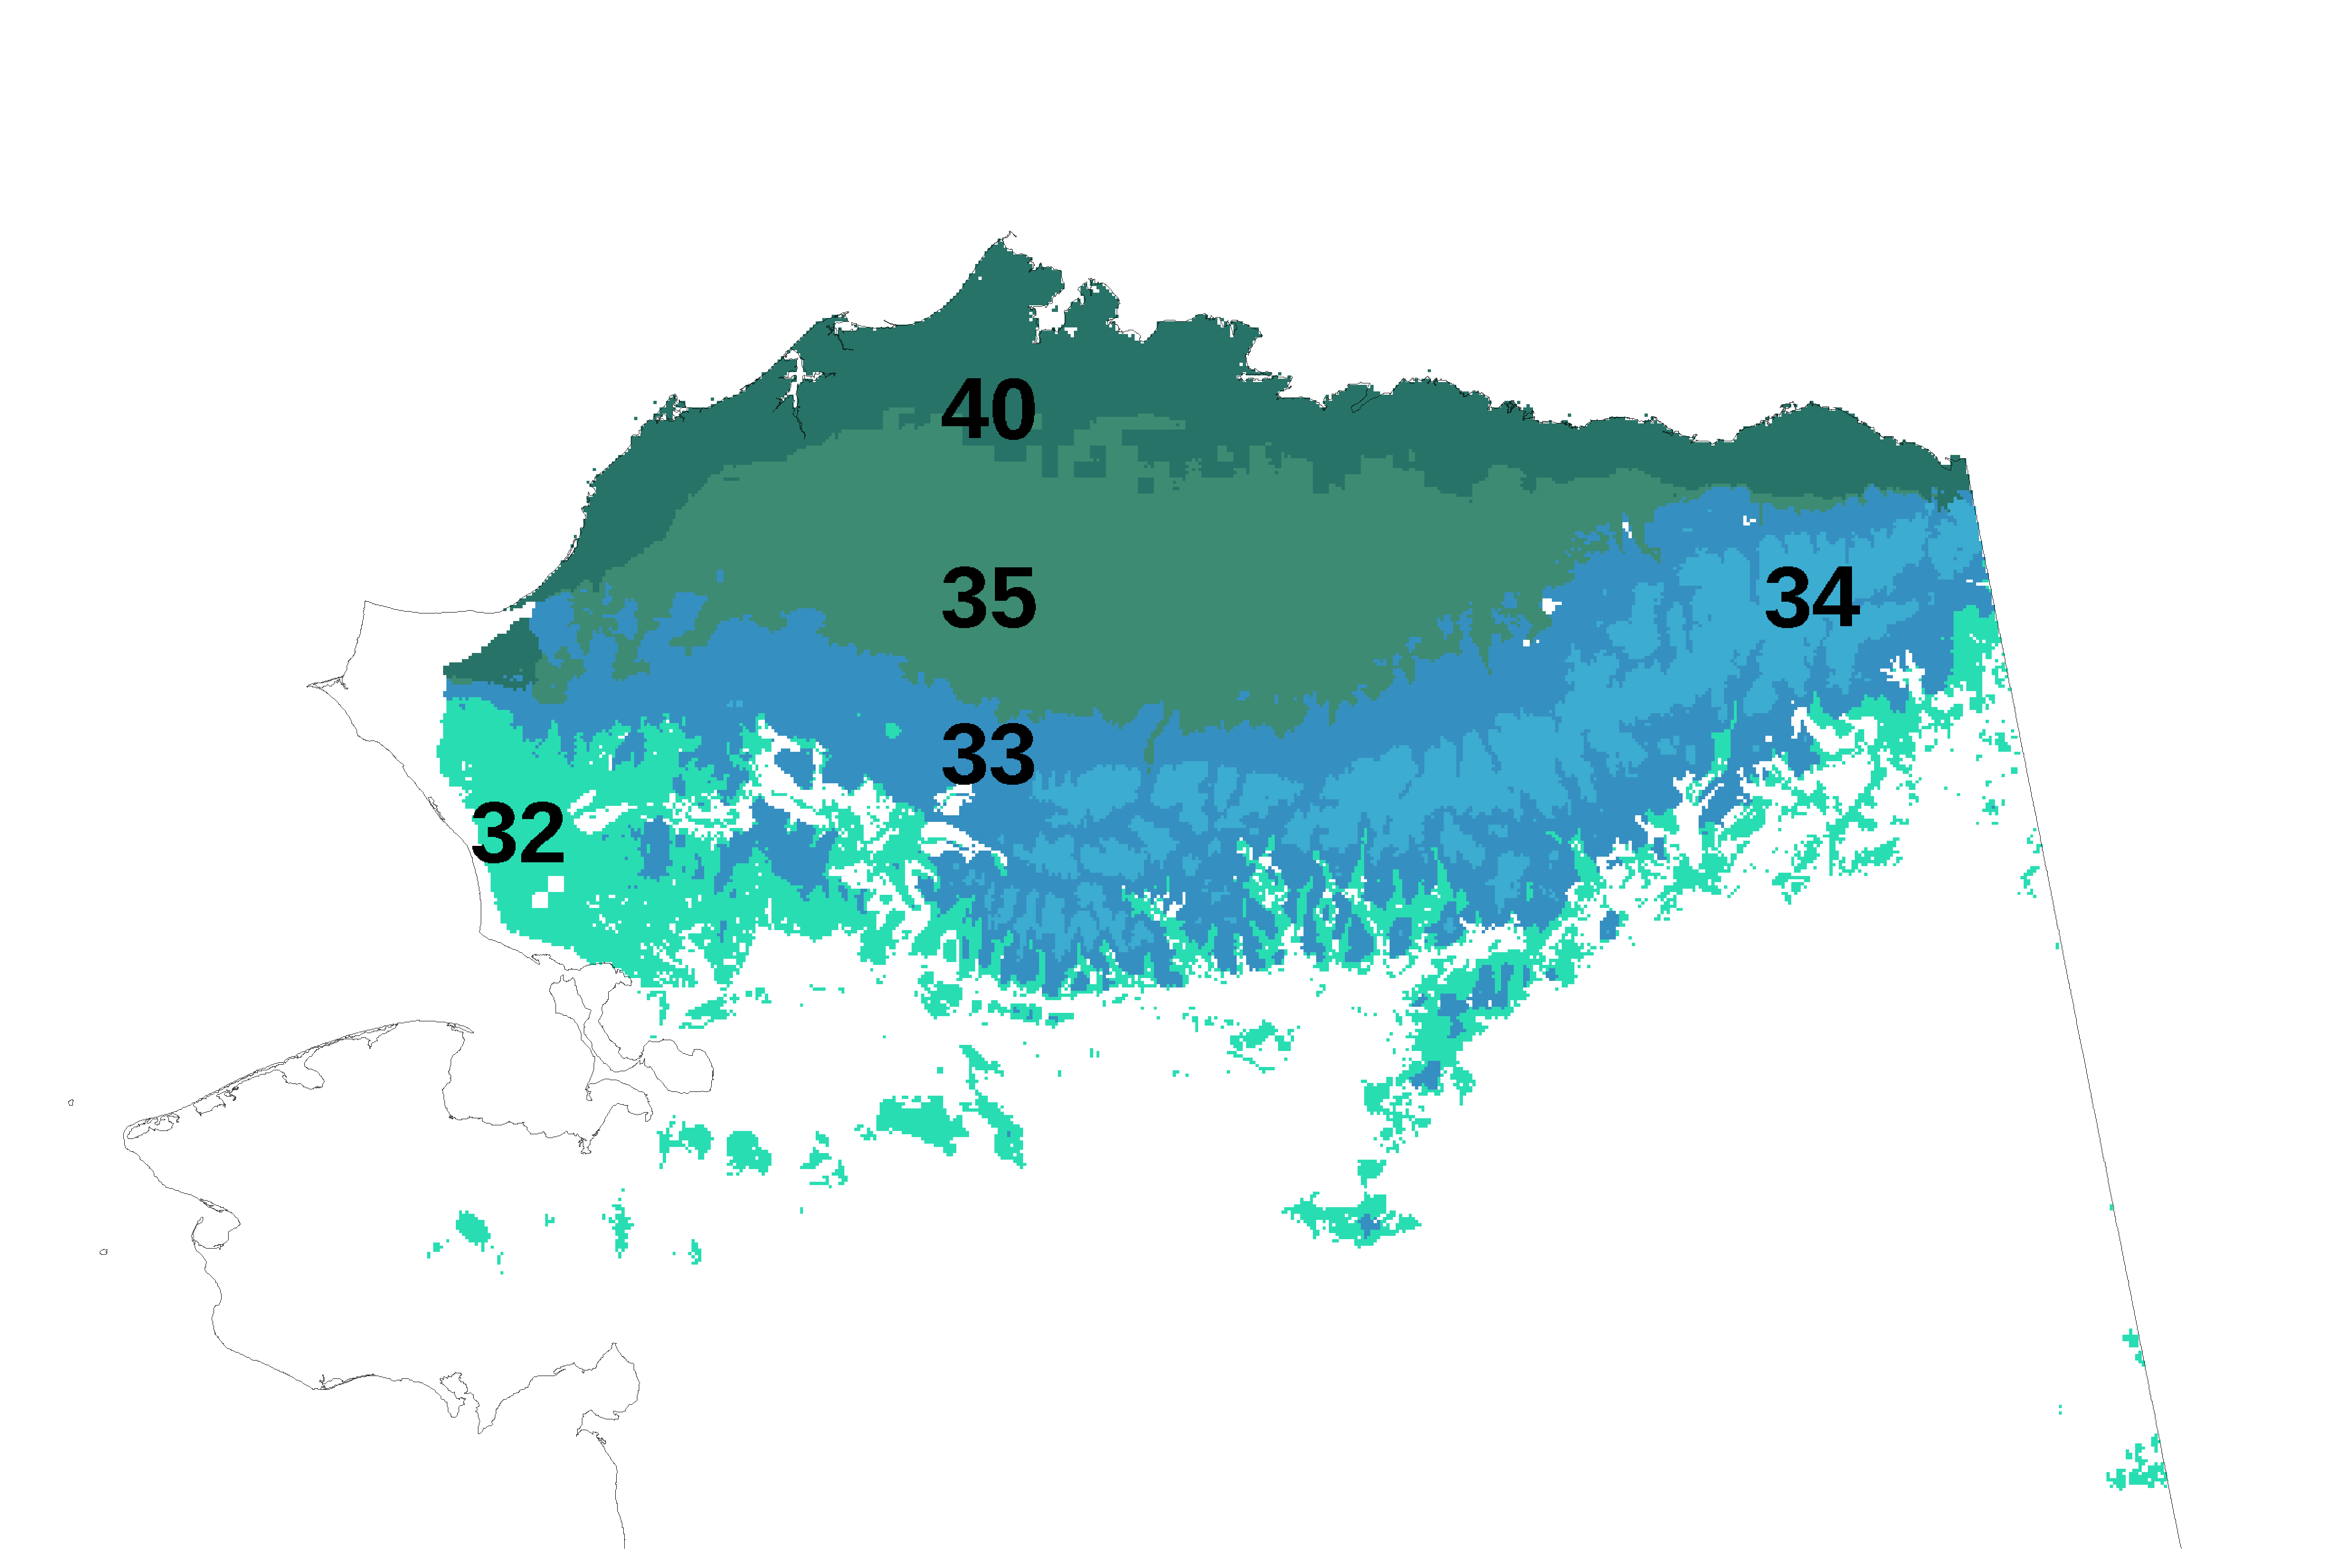
\includegraphics[width=0.315\textwidth]{ngee_figures/arctic_tundra_k50.pdf}\label{fig:k50_NSA}}
%%  \caption{\tiny A hierarchy of increasingly specific ecoregions for the
%% North Slope of Alaska emerge by increasing the level of division in the
%% MSTC algorithm.  MSTC cluster numbers are shown and the spatially
%% corresponding Level 2 ecological group or ecoregion defined by
%% \citet{Nowacki2001} is identified.}
%  \label{fig:k10+20+50_NSA}
%\end{figure}
%\end{frame}
%%%%%%%%%%%%%%%%%%%%%%%%%%%%%%%%%%%%%%%%%%%%%%%%%%%%%%%%%%%%%%%%%%%%%%%%%%%

\subsection[Representativeness]{Representativeness Analysis}

%%%%%%%%%%%%%%%%%%%%%%%%%%%%%%%%%%%%%%%%%%%%%%%%%%%%%%%%%%%%%%%%%%%%%%%%%%%%%%%
\begin{frame}
 \frametitle{NGEE Arctic Site Representativeness}
 \begin{itemize}
  \item This representativeness analysis uses the standardized
$n$-dimensional data space formed from all input data layers.
  \item In this data space, the Euclidean distance between a sampling
location (like Barrow) and every other point is calculated.
  \item These data space distances are then used to generate
grayscale maps showing the similarity, or lack thereof, of every
location to the sampling location.
  \item In the subsequent maps, white areas are well represented by
the sampling location or network, while dark and black areas
as poorly represented by the sampling location or network.
  \item This analysis assumes that the climate surrogates maintain
their predictive power and that no significant biological
adaptation occurs in the future.
 \end{itemize}
\end{frame}
%%%%%%%%%%%%%%%%%%%%%%%%%%%%%%%%%%%%%%%%%%%%%%%%%%%%%%%%%%%%%%%%%%%%%%%%%%%%%%%

%%%%%%%%%%%%%%%%%%%%%%%%%%%%%%%%%%%%%%%%%%%%%%%%%%%%%%%%%%%%%%%%%%%%%%%%%%%%%%%
\begin{frame}
 \frametitle{Present Representativeness of Barrow or ``Barrow-ness''}

 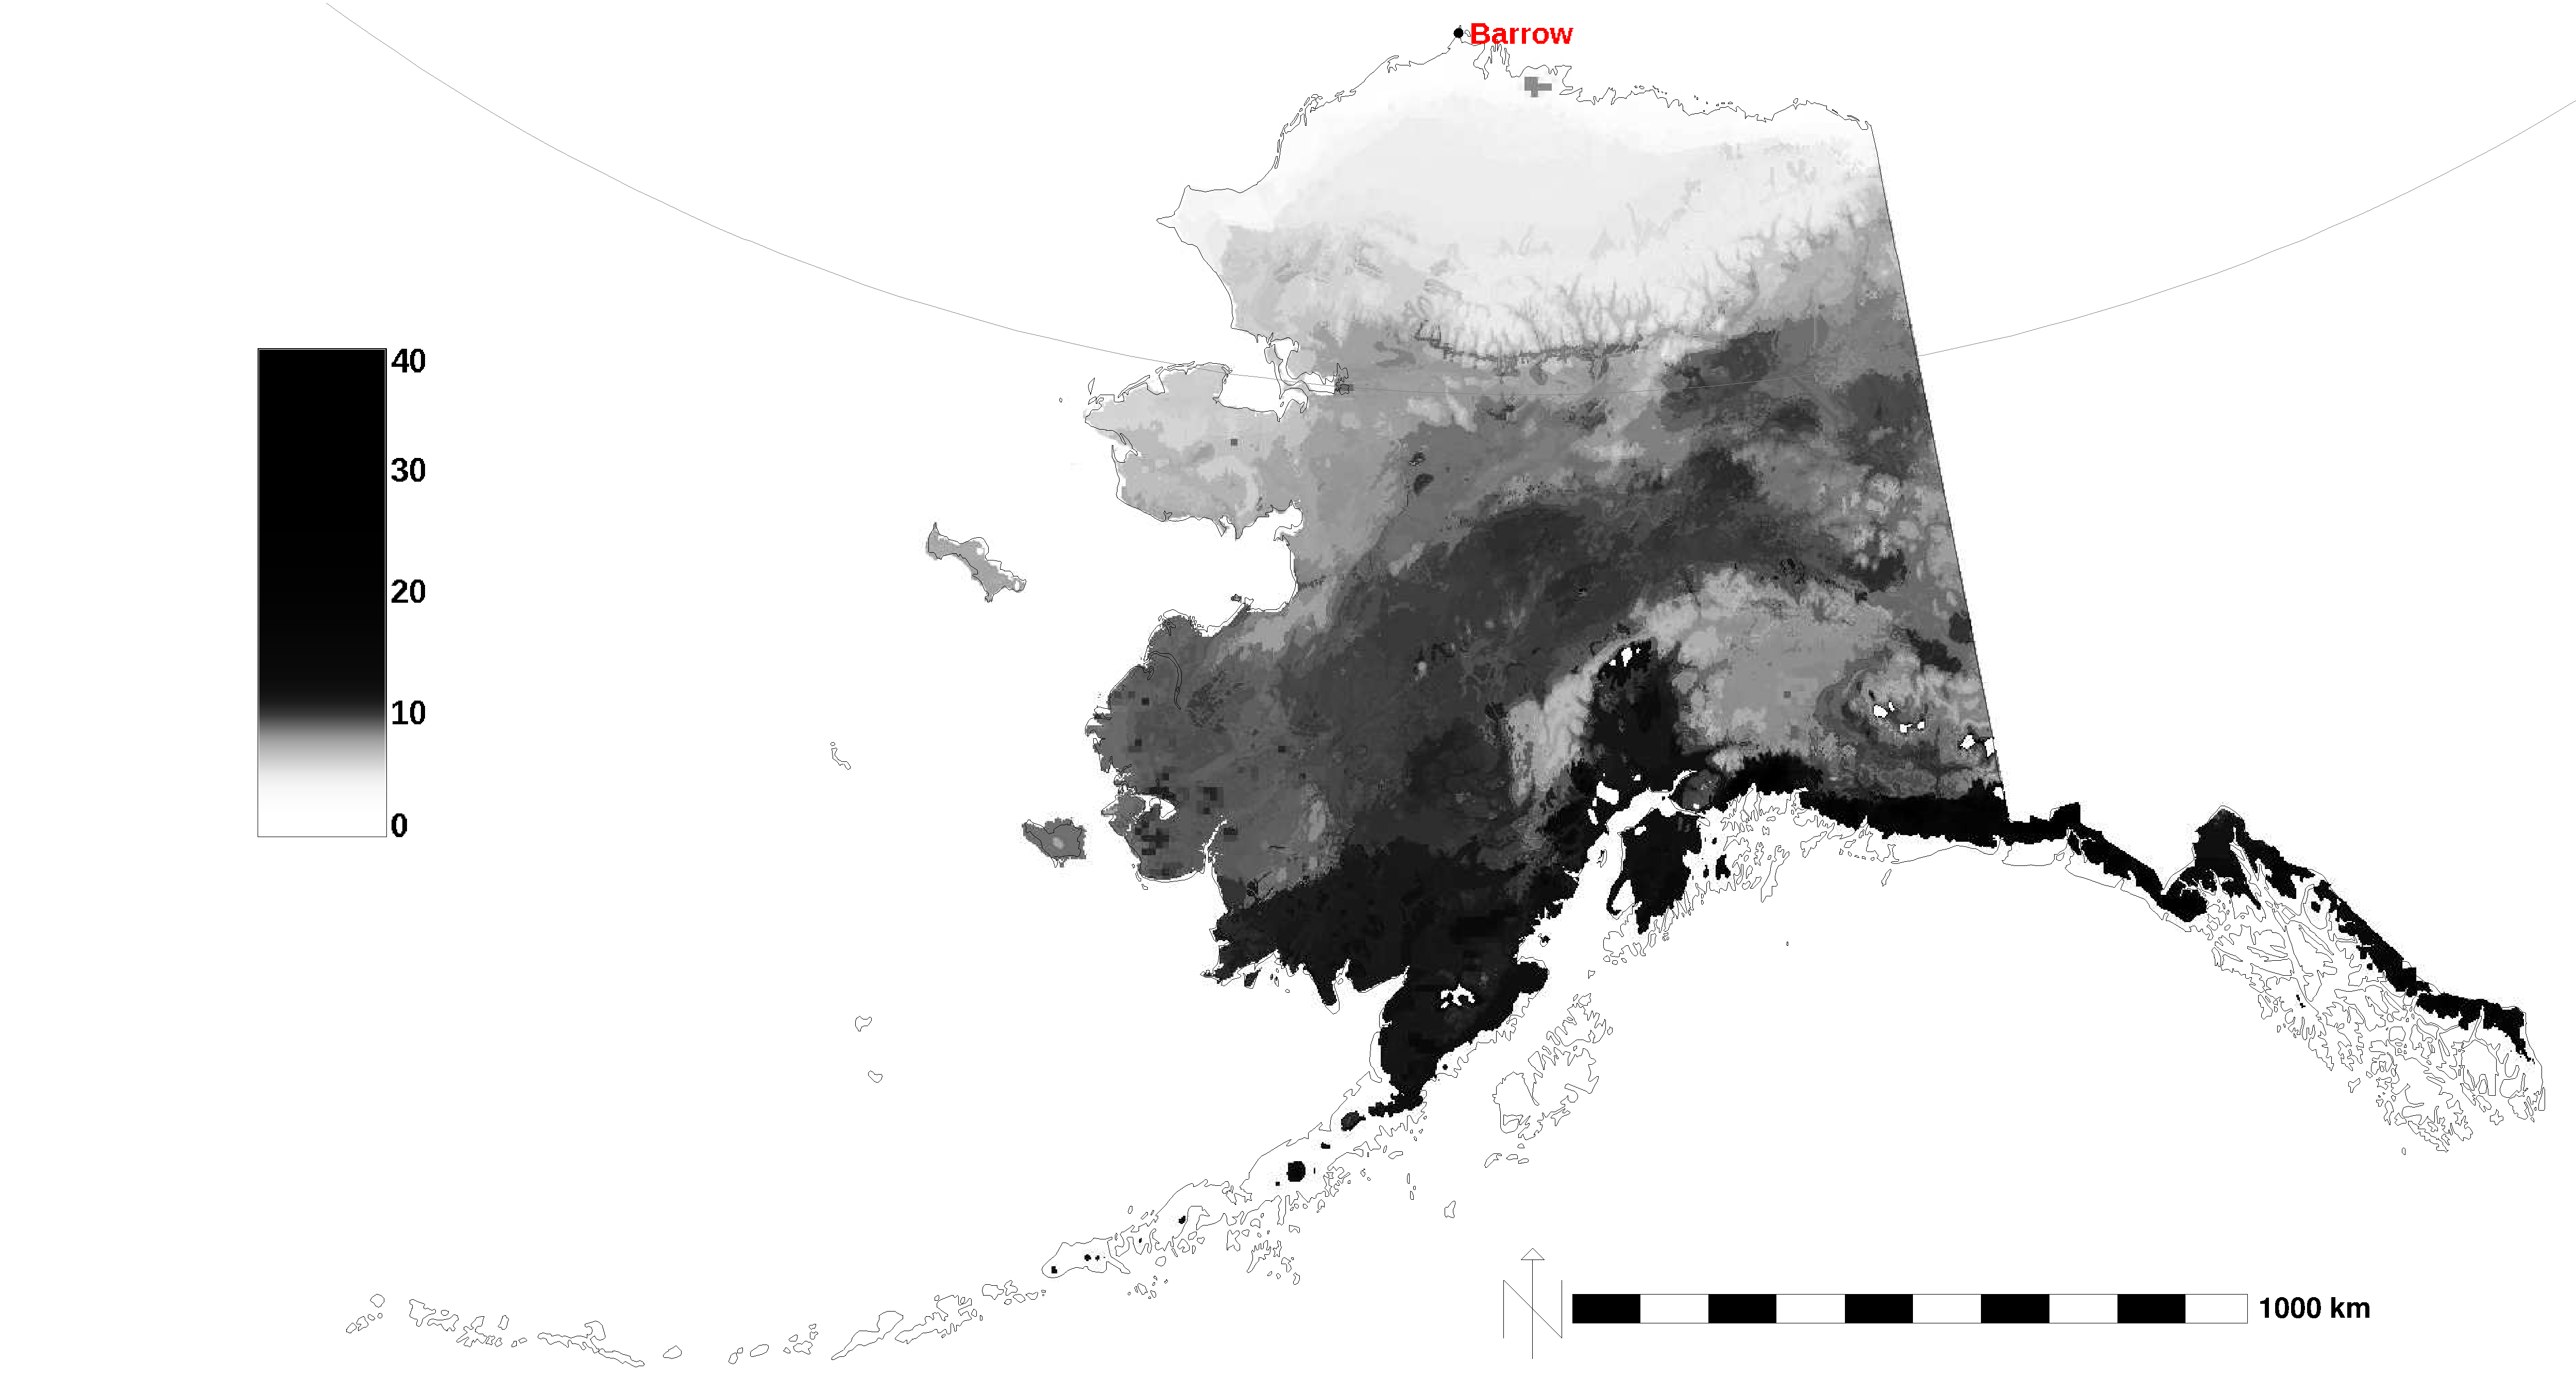
\includegraphics[width=\textwidth]{ngee_figures/alaska_2000_2009_dem_Feb2012_k1000ness_1sites.pdf} \\
  \vbox{\scriptsize\hfill\citep{Hoffman_LandscapeEcol_20131001}}
\medskip
Light-colored regions are well represented and dark-colored regions are
poorly represented by the sampling location listed in \textbf{\color{red}red}.

\end{frame}
%%%%%%%%%%%%%%%%%%%%%%%%%%%%%%%%%%%%%%%%%%%%%%%%%%%%%%%%%%%%%%%%%%%%%%%%%%%%%%%
%\begin{frame}
% \frametitle{Present vs. Future Barrow-ness}
% \vskip-0.15in
% \setlength{\tabcolsep}{0pt}
% \begin{figure}
%   \begin{tabular}{cc}
%   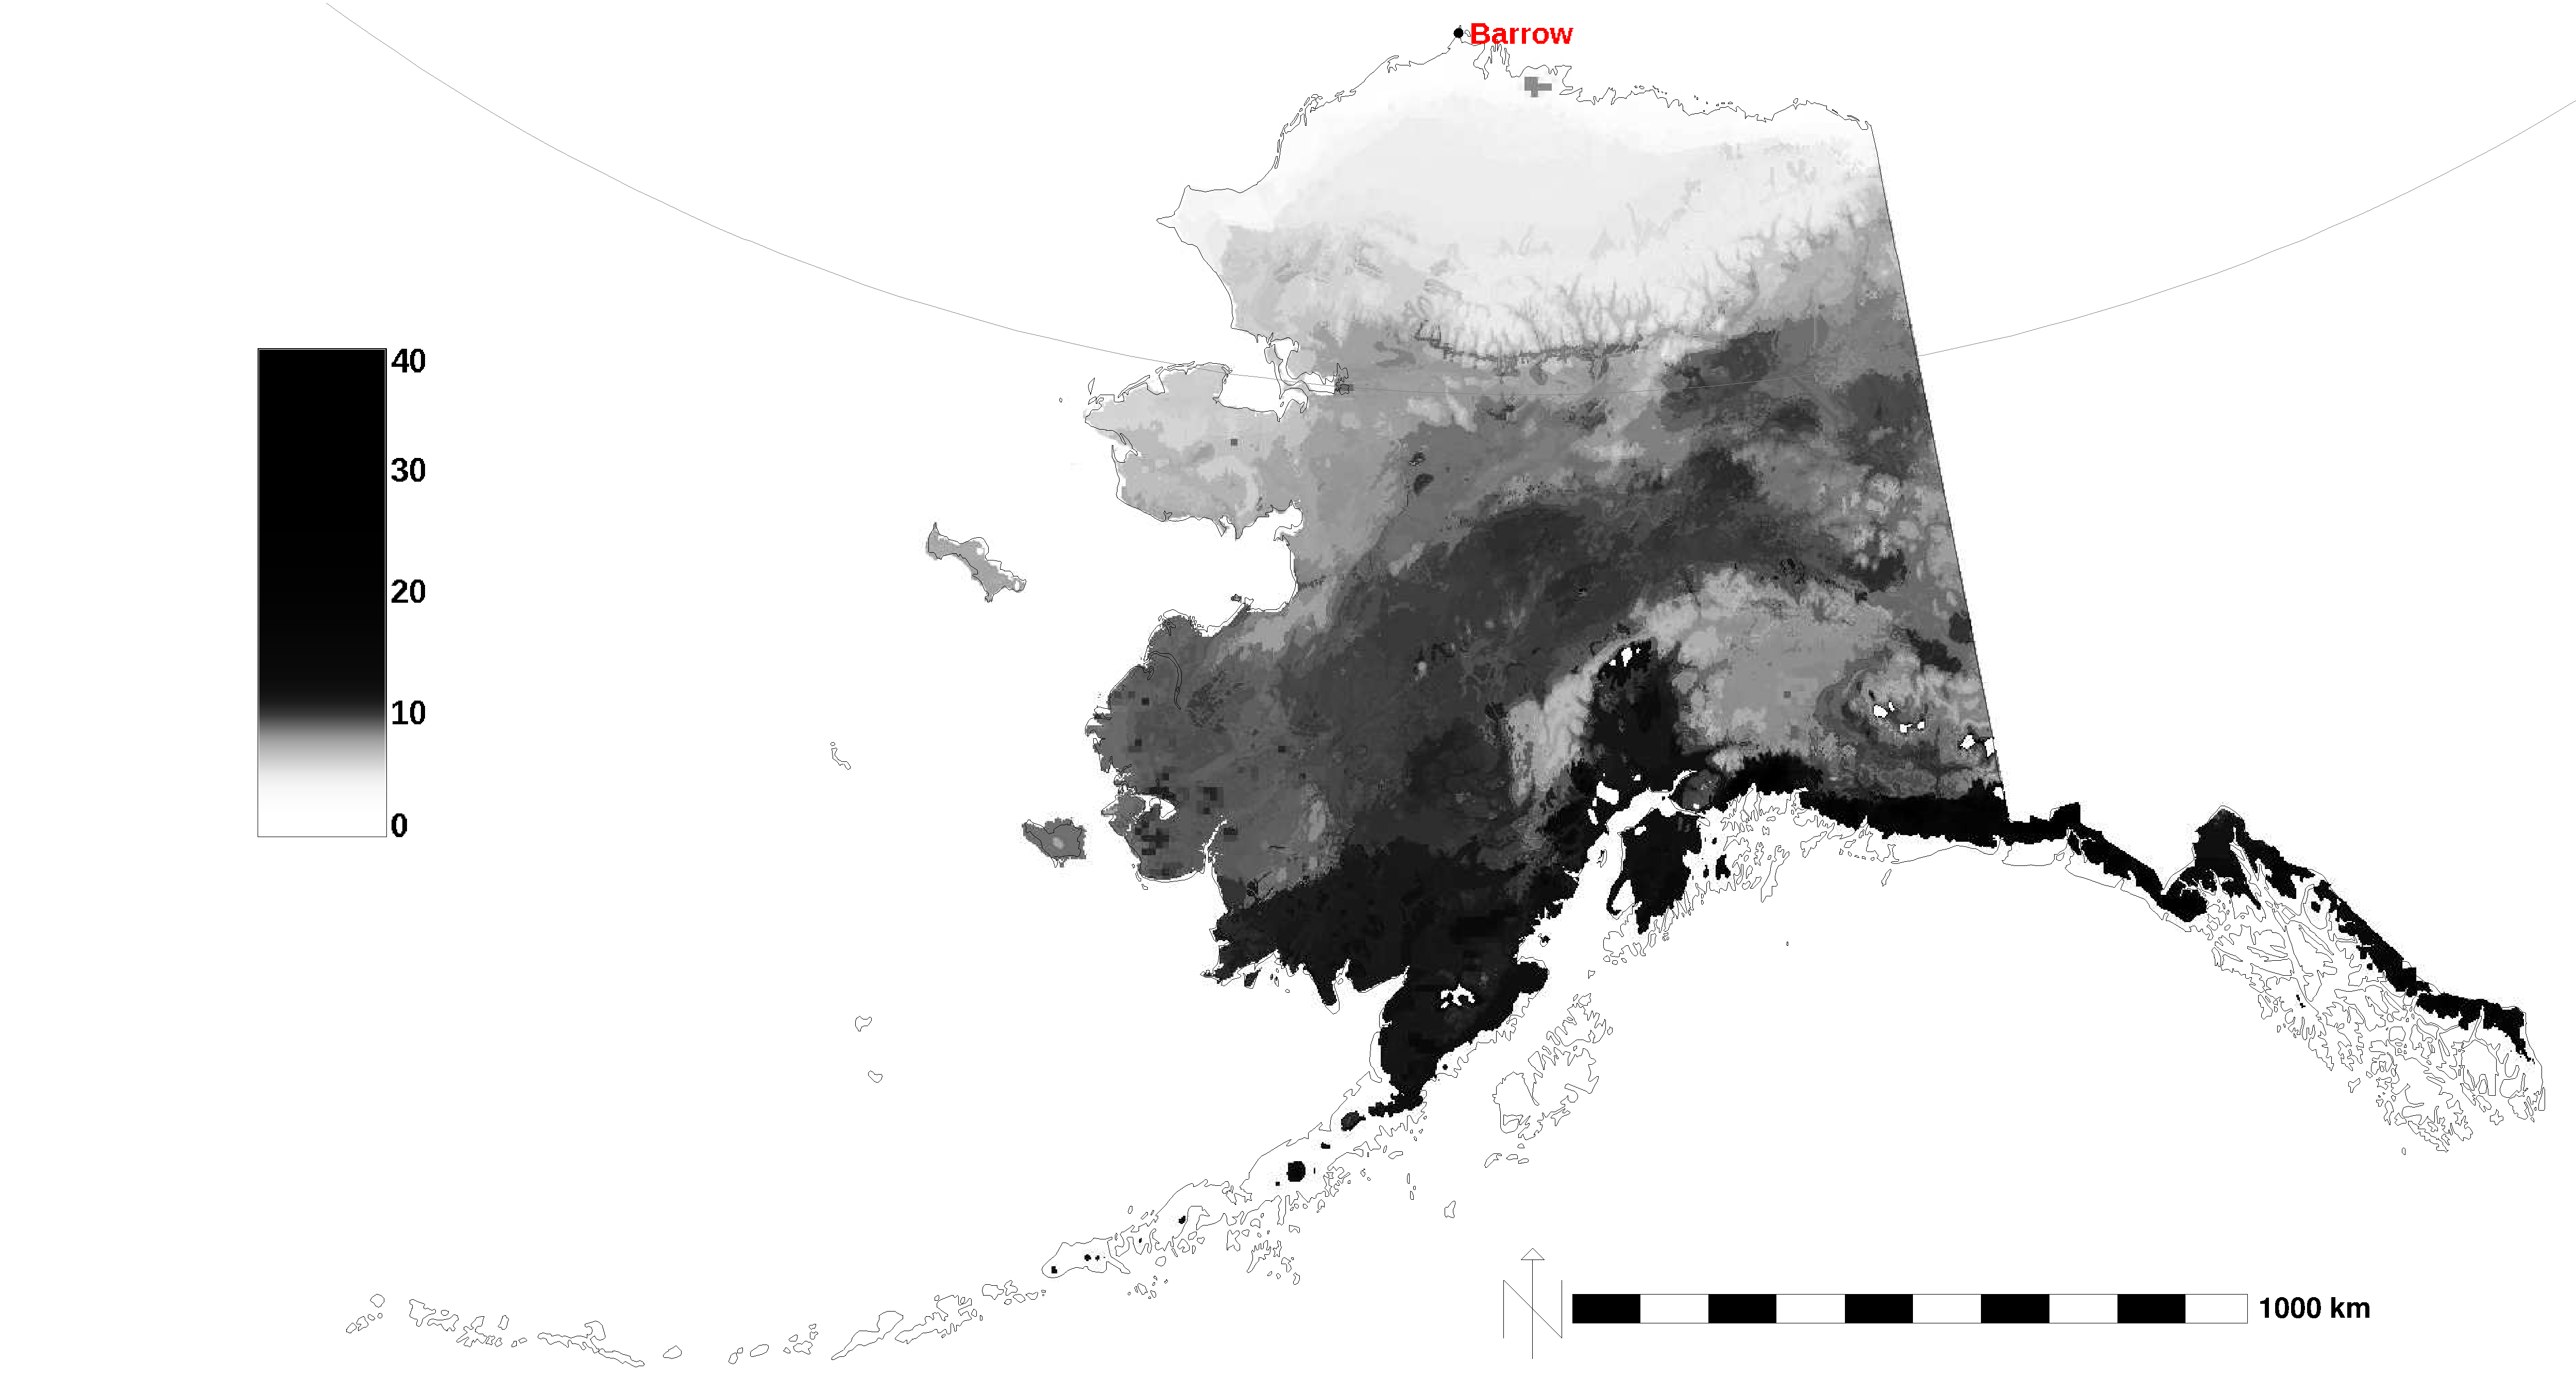
\includegraphics[width=0.50\textwidth]{ngee_figures/alaska_2000_2009_dem_Feb2012_k1000ness_1sites.pdf} &
%   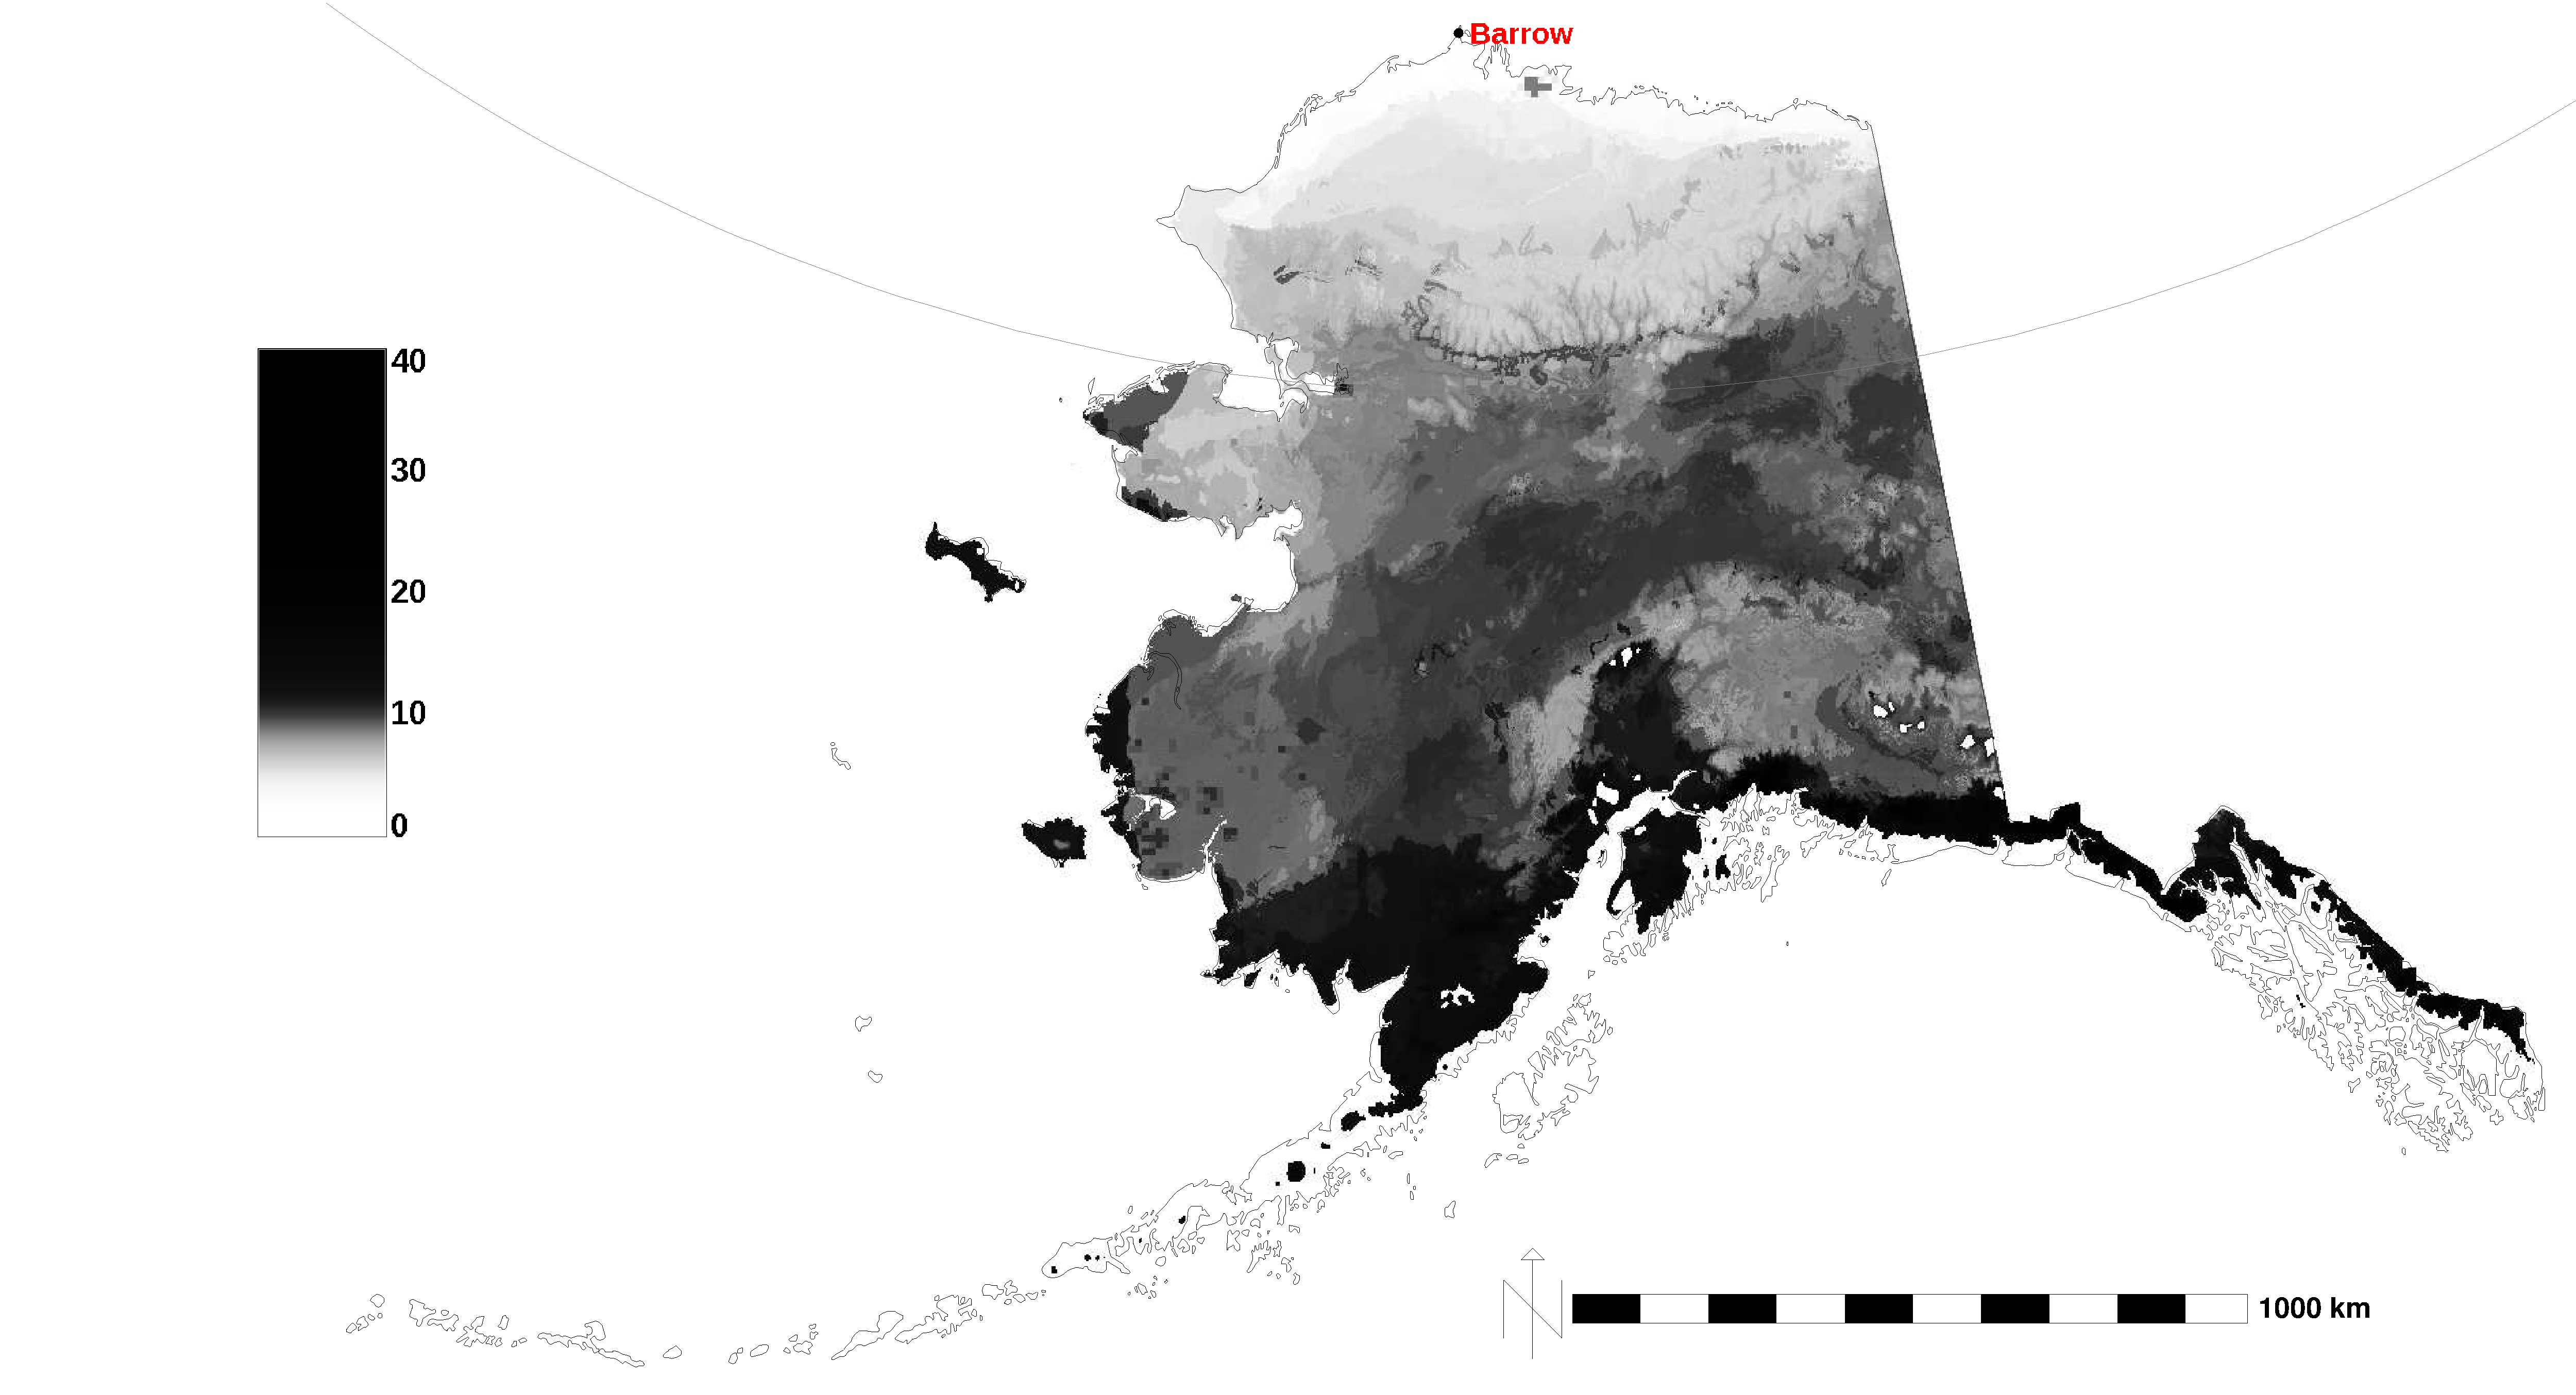
\includegraphics[width=0.50\textwidth]{ngee_figures/alaska_2090_2099_dem_Feb2012_k1000ness_1sites.pdf} \\
%   2000--2009 & 2090--2099 \\
%   \end{tabular}
%  %\caption{Cluster analysis.}
%  \label{fig:barrowness}
% \end{figure}
%
%As environmental conditions change, due primarily to increasing
%temperatures, climate gradients increase and the representativeness
%of Barrow will be diminished in the future.
%
%\end{frame}
%%%%%%%%%%%%%%%%%%%%%%%%%%%%%%%%%%%%%%%%%%%%%%%%%%%%%%%%%%%%%%%%%%%%%%%%%%%%
%
%%%%%%%%%%%%%%%%%%%%%%%%%%%%%%%%%%%%%%%%%%%%%%%%%%%%%%%%%%%%%%%%%%%%%%%%%%%%
%\begin{frame}
% \frametitle{Council and Prudhoe Bay Representativeness}
% \vskip-0.15in
% \setlength{\tabcolsep}{0pt}
% \begin{figure}
%   \begin{tabular}{cc}
%   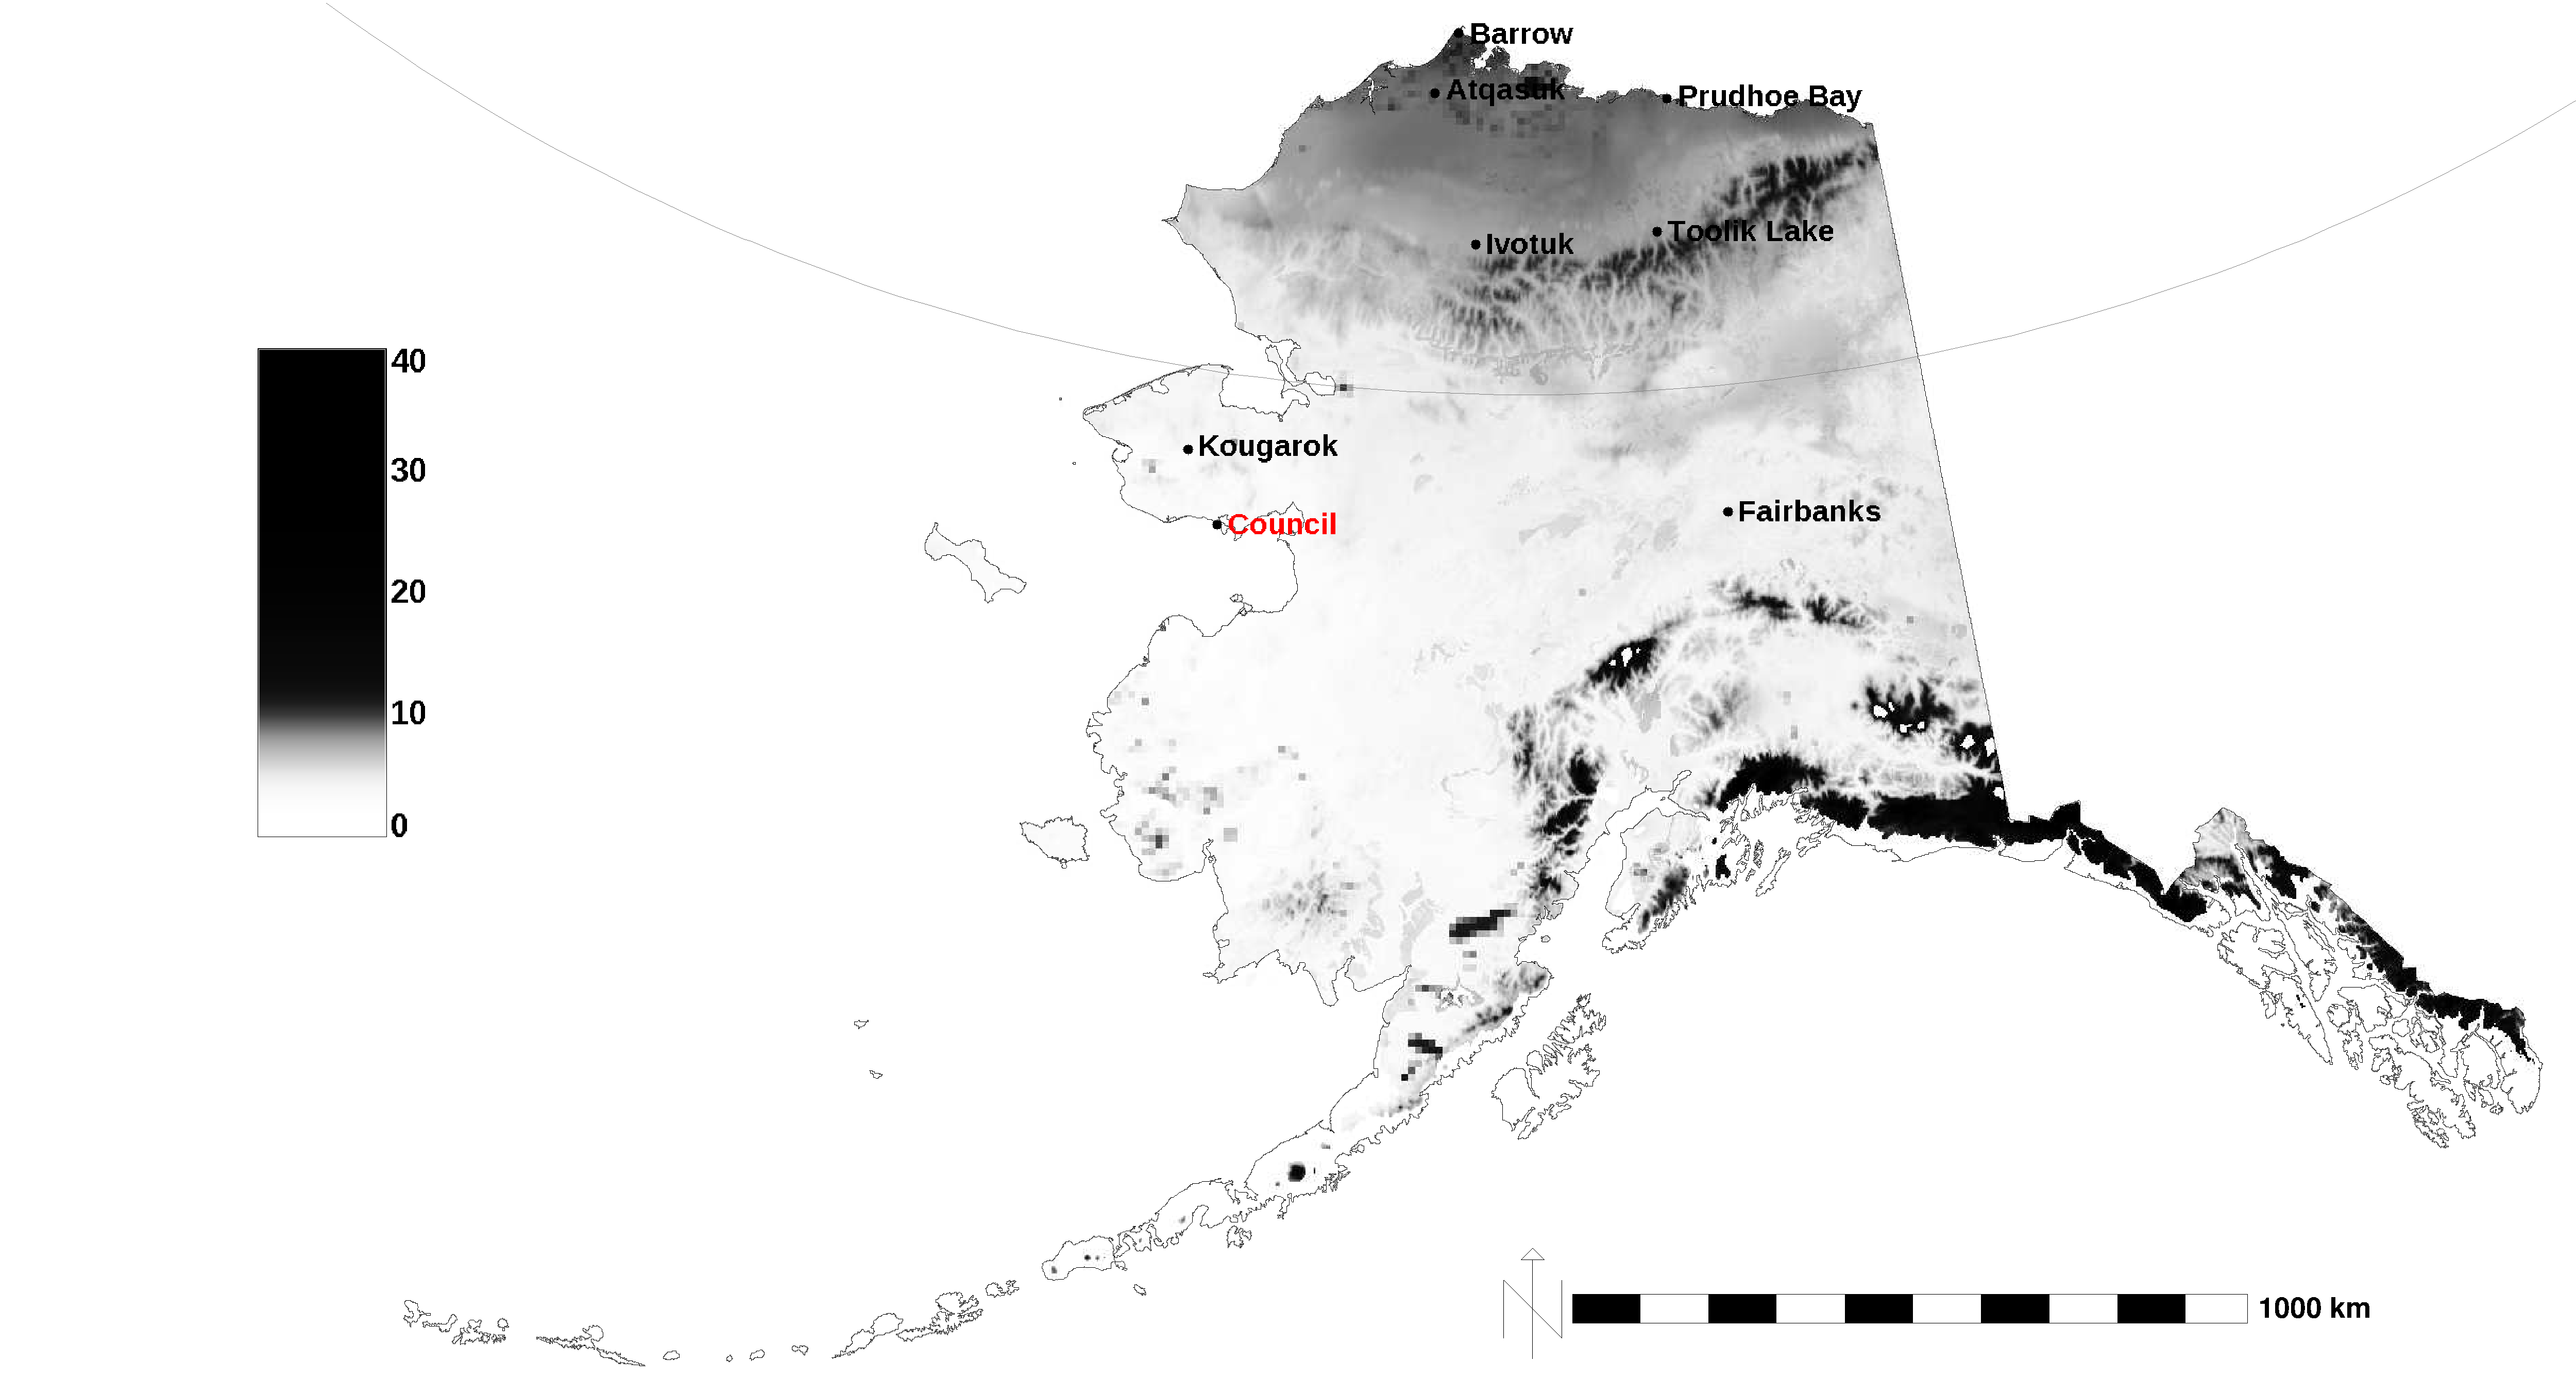
\includegraphics[width=0.50\textwidth]{ngee_figures/Councilness_2000_2009_on_2000_2009_point_global_dem_Feb2012.pdf} &
%   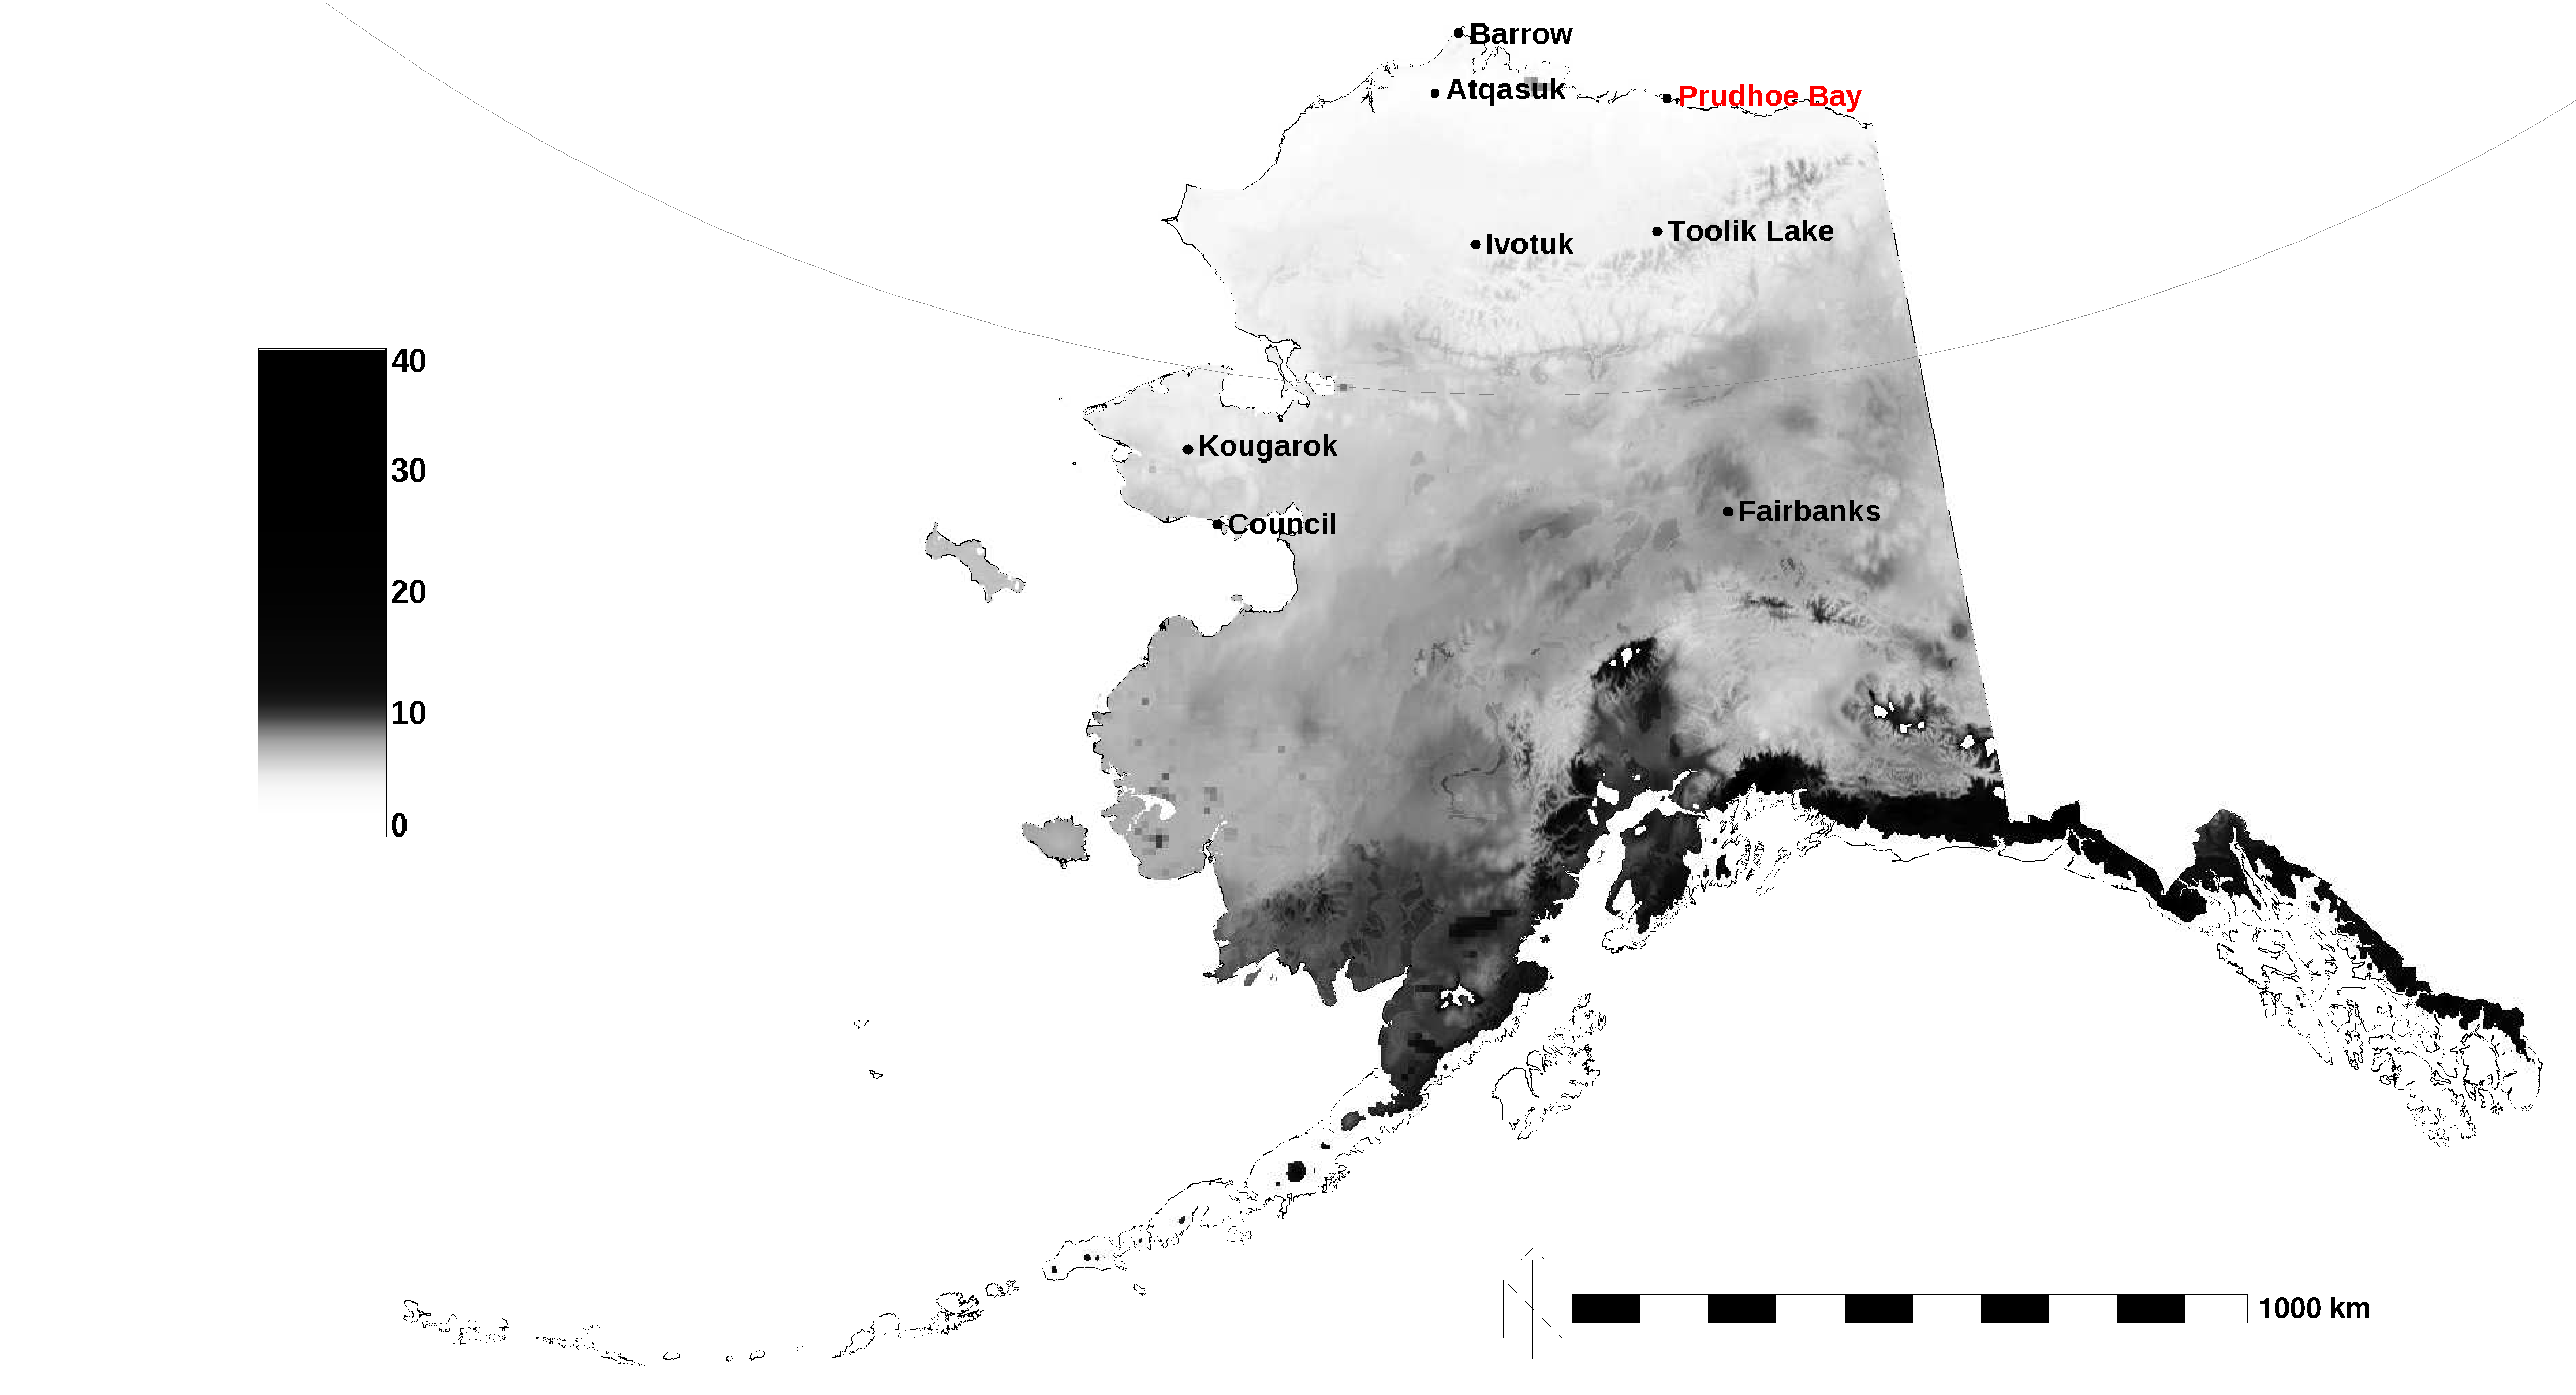
\includegraphics[width=0.50\textwidth]{ngee_figures/Prudhoe_bayness_2000_2009_on_2000_2009_point_global_dem_Feb2012.pdf} \\
%   Council & Prudhoe Bay \\
%   \end{tabular}
%  %\caption{Cluster analysis.}
%  \label{fig:council_and_prudhoe_bay}
% \end{figure}
%
%Representativeness analysis was performed for sites at Barrow, Council, Atqasuk,
%Ivotuk, Kougarok, Prudhoe Bay, Toolik Lake, and Fairbanks.
%
%\end{frame}
%%%%%%%%%%%%%%%%%%%%%%%%%%%%%%%%%%%%%%%%%%%%%%%%%%%%%%%%%%%%%%%%%%%%%%%%%%%%
%
%%%%%%%%%%%%%%%%%%%%%%%%%%%%%%%%%%%%%%%%%%%%%%%%%%%%%%%%%%%%%%%%%%%%%%%%%%%
\begin{frame}
 \frametitle{Network Representativeness: Barrow + Council}
 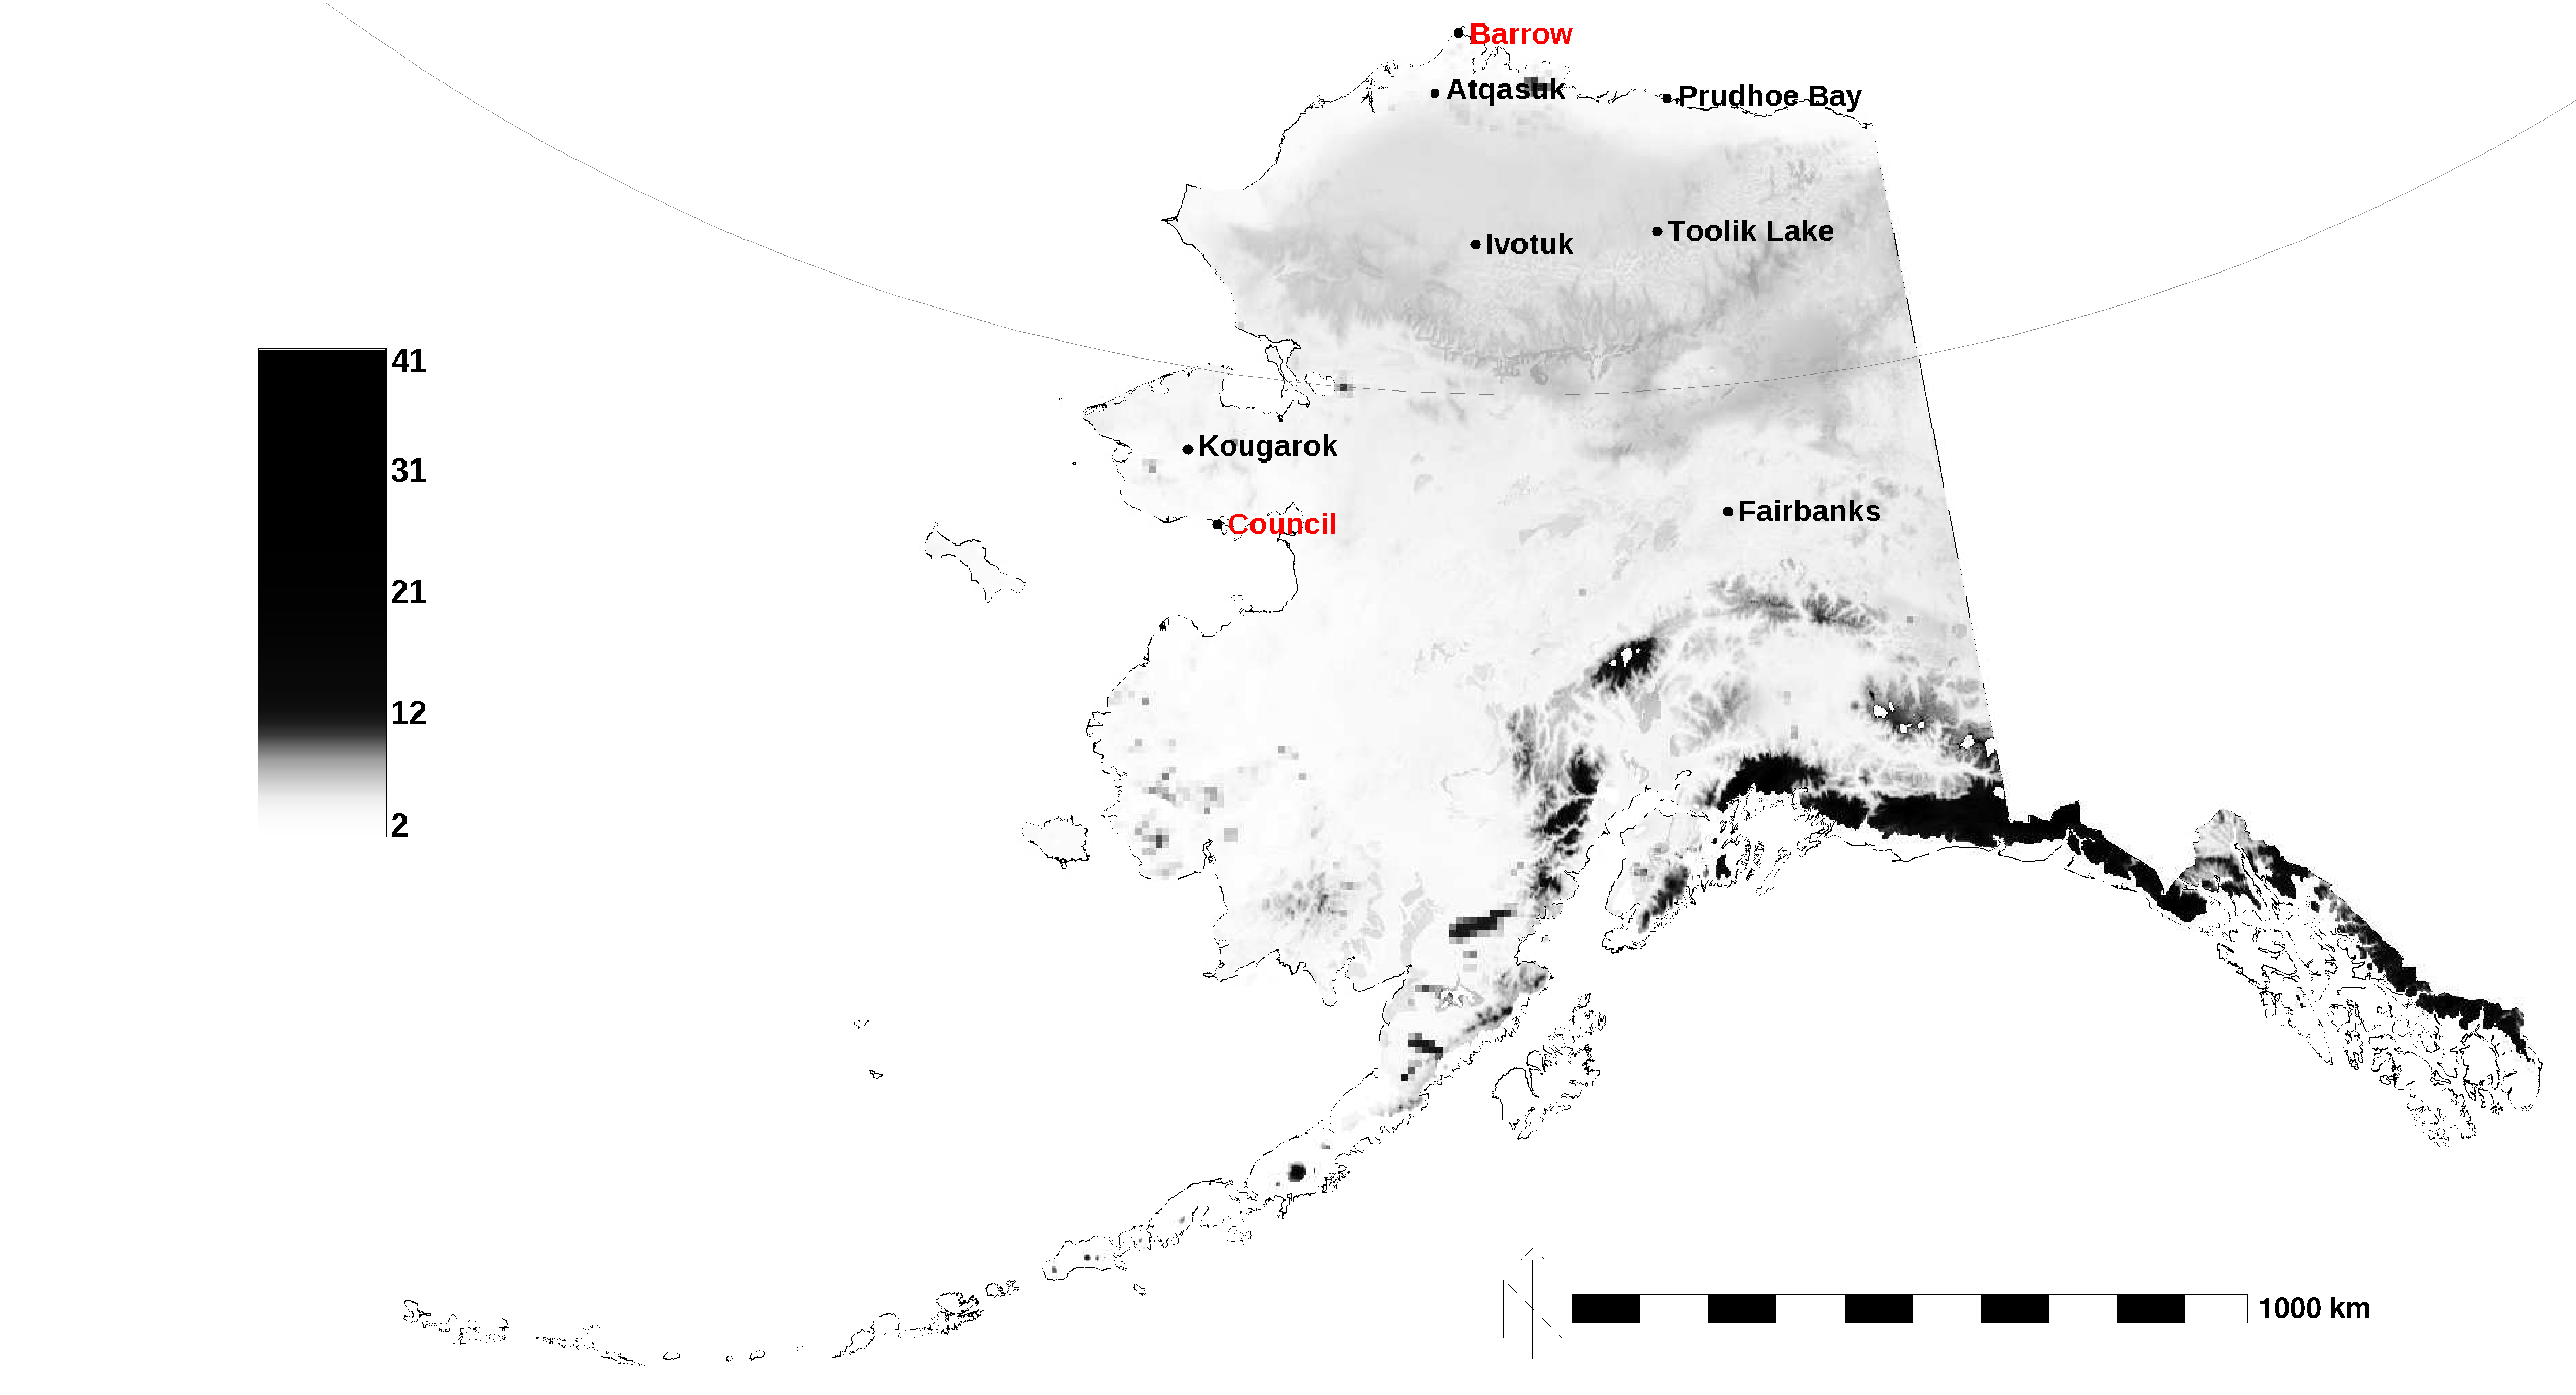
\includegraphics[width=\textwidth]{ngee_figures/Barrow-Councilness_2000-2009_on_2000-2009_point_global_dem_Feb2012_barscale.pdf} \\
  \vbox{\scriptsize\hfill\citep{Hoffman_LandscapeEcol_20131001}}

\medskip
Light-colored regions are well represented and dark-colored regions are
poorly represented by the sampling location listed in \textbf{\color{red}red}.
\end{frame}
%%%%%%%%%%%%%%%%%%%%%%%%%%%%%%%%%%%%%%%%%%%%%%%%%%%%%%%%%%%%%%%%%%%%%%%%%%%
%
%%%%%%%%%%%%%%%%%%%%%%%%%%%%%%%%%%%%%%%%%%%%%%%%%%%%%%%%%%%%%%%%%%%%%%%%%%%%
\begin{frame}
 \frametitle{Network Representativeness: All 8 Sites}
 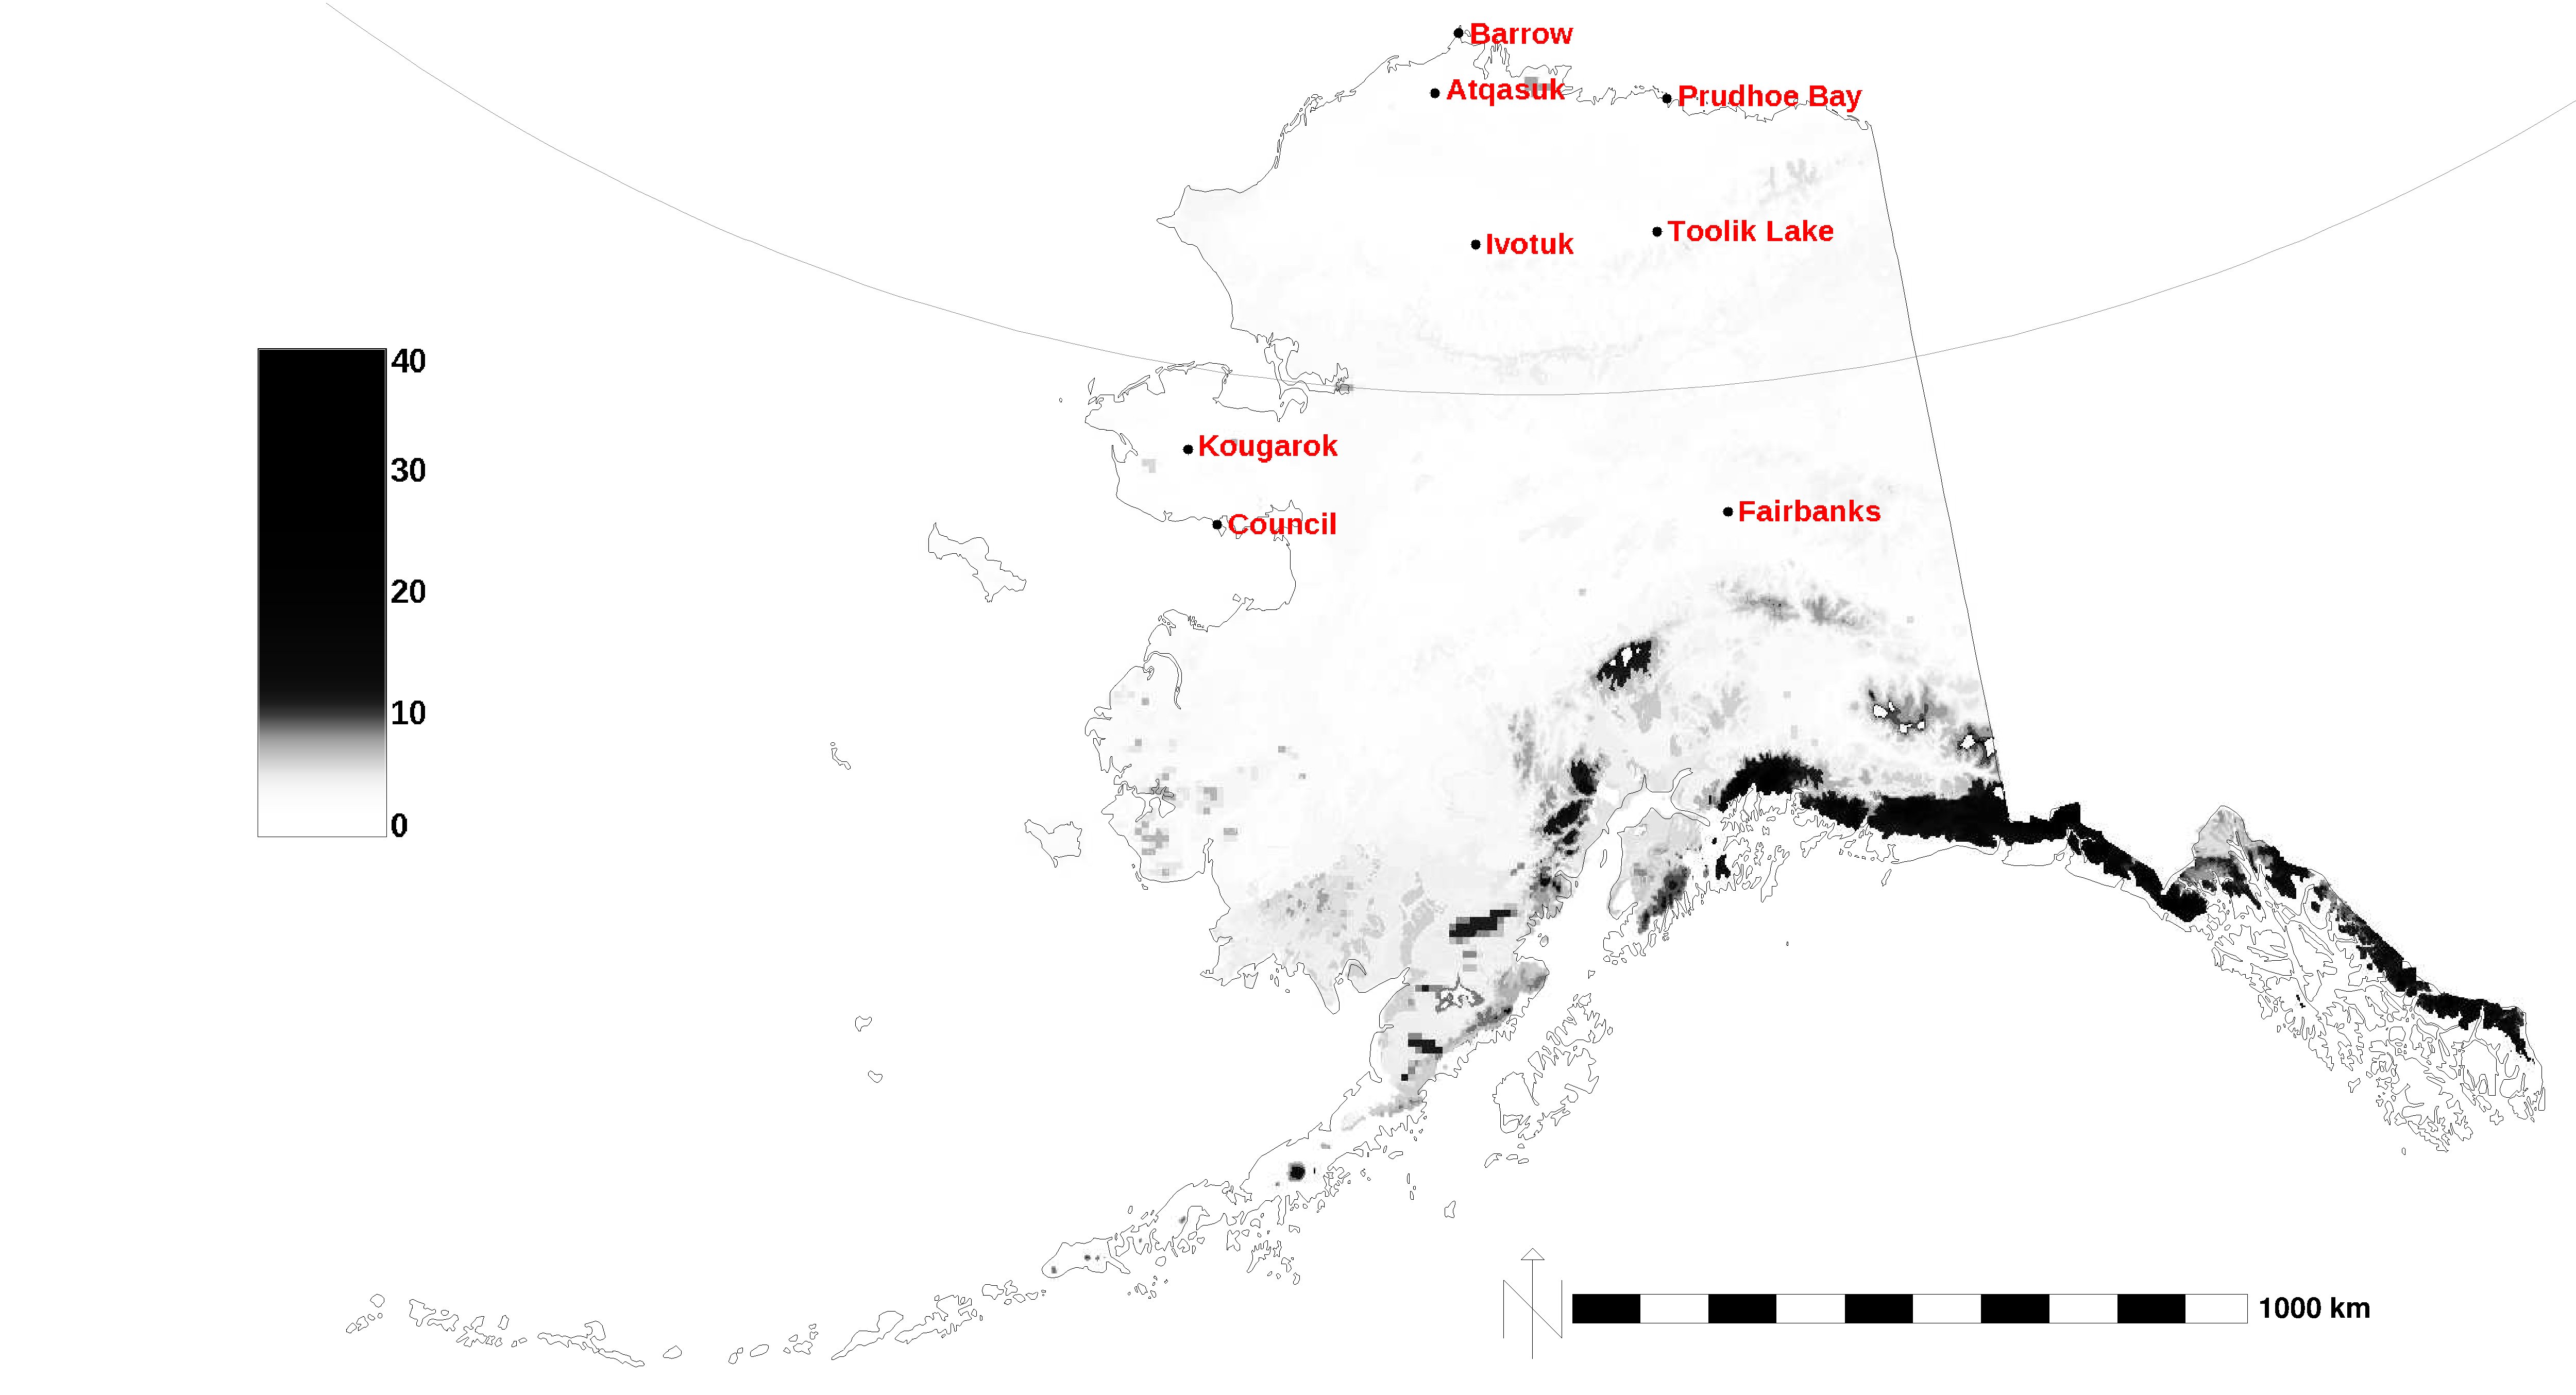
\includegraphics[width=\textwidth]{ngee_figures/alaska_2000_2009_dem_Feb2012_k1000ness_8sites.pdf} \\
  \vbox{\scriptsize\hfill\citep{Hoffman_LandscapeEcol_20131001}}

\medskip
Light-colored regions are well represented and dark-colored regions are
poorly represented by the sampling location listed in \textbf{\color{red}red}.
\end{frame}
%%%%%%%%%%%%%%%%%%%%%%%%%%%%%%%%%%%%%%%%%%%%%%%%%%%%%%%%%%%%%%%%%%%%%%%%%%%

%%%%%%%%%%%%%%%%%%%%%%%%%%%%%%%%%%%%%%%%%%%%%%%%%%%%%%%%%%%%%%%%%%%%%%%%%%%
% HoJo
%%%%%%%%%%%%%%%%%%%%%%%%%%%%%%%%%%%%%%%%%%%%%%%%%%%%%%%%%%%%%%%%%%%%%%%%%%%
\begin{frame}
 \frametitle{State Space Dissimilarities: 8 Sites, Present (2000--2009)}
 
\begin{table}
 \footnotesize\setlength{\tabcolsep}{2pt}
 \centering
  \caption{Site state space distances for the present (2000--2009) with DEM}
  \label{tbl:hojo_present}
  \begin{tabular}{r s s s s s s s}
   \toprule
   &  &  &  & \multicolumn{1}{c}{Toolik} &  & \multicolumn{1}{c}{Prudhoe} &  \\
   \multicolumn{1}{c}{\textbf{Sites}} & \multicolumn{1}{c}{Council} & \multicolumn{1}{c}{Atqasuk} & \multicolumn{1}{c}{Ivotuk} & \multicolumn{1}{c}{Lake} & \multicolumn{1}{c}{Kougarok} & \multicolumn{1}{c}{Bay} & \multicolumn{1}{c}{Fairbanks} \\
   \midrule
        Barrow &        9.13 &        4.53 &        5.90 &        5.87 &        7.98 &        3.57 &       12.16 \\
       Council &             &        8.69 &        6.37 &        7.00 &        2.28 &        8.15 &        5.05 \\
       Atqasuk &             &             &        5.18 &        5.23 &        7.79 &        1.74 &       10.66 \\
        Ivotuk &             &             &             &        1.81 &        5.83 &        4.48 &        7.90 \\
   Toolik Lake &             &             &             &             &        6.47 &        4.65 &        8.70 \\
      Kougarok &             &             &             &             &             &        7.25 &        5.57 \\
   Prudhoe Bay &             &             &             &             &             &             &       10.38 \\
   \bottomrule
  \end{tabular}
\end{table}


\end{frame}
%%%%%%%%%%%%%%%%%%%%%%%%%%%%%%%%%%%%%%%%%%%%%%%%%%%%%%%%%%%%%%%%%%%%%%%%%%%

%%%%%%%%%%%%%%%%%%%%%%%%%%%%%%%%%%%%%%%%%%%%%%%%%%%%%%%%%%%%%%%%%%%%%%%%%%%
\begin{frame}
 \frametitle{State Space Dissimilarities: 8 Sites, Future (2090--2099)}
 
\begin{table}
 \footnotesize\setlength{\tabcolsep}{2pt}
 \centering
  \caption{Site state space distances for the future (2090--2099) with DEM}
  \label{tbl:hojo_future}
  \begin{tabular}{r s s s s s s s}
   \toprule
   &  &  &  & \multicolumn{1}{c}{Toolik} &  & \multicolumn{1}{c}{Prudhoe} &  \\
   \multicolumn{1}{c}{\textbf{Sites}} & \multicolumn{1}{c}{Council} & \multicolumn{1}{c}{Atqasuk} & \multicolumn{1}{c}{Ivotuk} & \multicolumn{1}{c}{Lake} & \multicolumn{1}{c}{Kougarok} & \multicolumn{1}{c}{Bay} & \multicolumn{1}{c}{Fairbanks} \\
   \midrule
        Barrow &        8.87 &        4.89 &        6.88 &        6.94 &        8.04 &        4.18 &       11.95 \\
       Council &             &        8.82 &        6.93 &        7.74 &        2.43 &        8.24 &        5.66 \\
       Atqasuk &             &             &        5.86 &        5.84 &        8.15 &        2.30 &       10.16 \\
        Ivotuk &             &             &             &        2.01 &        7.27 &        4.75 &        7.51 \\
   Toolik Lake &             &             &             &             &        7.81 &        5.00 &        8.33 \\
      Kougarok &             &             &             &             &             &        7.89 &        6.42 \\
   Prudhoe Bay &             &             &             &             &             &             &        9.81 \\
   \bottomrule
  \end{tabular}
\end{table}


\end{frame}
%%%%%%%%%%%%%%%%%%%%%%%%%%%%%%%%%%%%%%%%%%%%%%%%%%%%%%%%%%%%%%%%%%%%%%%%%%%%

%%%%%%%%%%%%%%%%%%%%%%%%%%%%%%%%%%%%%%%%%%%%%%%%%%%%%%%%%%%%%%%%%%%%%%%%%%%
\begin{frame}
 \frametitle{State Space Dissimilarities: 8 Sites, Present and Future}
 
\begin{table}
 \scriptsize\setlength{\tabcolsep}{1pt}
 \centering
  \caption{Site state space distances between the present (2000--2009) and the future (2090--2099) with DEM}
  \label{tbl:hojo_present_future}
  \begin{tabular}{c r s s s s s s s s}
   \toprule
    &  & \multicolumn{8}{c}{\textit{Future (2090--2099)}} \\
    & &  &  &  &  & \multicolumn{1}{c}{Toolik} &  & \multicolumn{1}{c}{Prudhoe} &  \\
    & \multicolumn{1}{c}{\textbf{Sites}} & \multicolumn{1}{c}{Barrow} & \multicolumn{1}{c}{Council} & \multicolumn{1}{c}{Atqasuk} & \multicolumn{1}{c}{Ivotuk} & \multicolumn{1}{c}{Lake} & \multicolumn{1}{c}{Kougarok} & \multicolumn{1}{c}{Bay} & \multicolumn{1}{c}{Fairbanks} \\
   \midrule
   \multirow{8}{*}{\begin{sideways}\textit{Present (2000--2009)}\end{sideways}}
    &      Barrow &        3.31 &        9.67 &        4.63 &        6.05 &        5.75 &        9.02 &        3.69 &       11.67 \\
    &     Council &        8.38 &        1.65 &        8.10 &        5.91 &        6.87 &        3.10 &        7.45 &        5.38 \\
    &     Atqasuk &        6.01 &        9.33 &        2.42 &        5.46 &        5.26 &        8.97 &        2.63 &       10.13 \\
    &      Ivotuk &        7.06 &        7.17 &        5.83 &        1.53 &        2.05 &        7.25 &        4.87 &        7.40 \\
    & Toolik Lake &        7.19 &        7.67 &        6.07 &        2.48 &        1.25 &        7.70 &        5.23 &        8.16 \\
    &    Kougarok &        7.29 &        3.05 &        6.92 &        5.57 &        6.31 &        2.51 &        6.54 &        5.75 \\
    & Prudhoe Bay &        5.29 &        8.80 &        3.07 &        4.75 &        4.69 &        8.48 &        1.94 &        9.81 \\
    &   Fairbanks &       12.02 &        5.49 &       10.36 &        7.83 &        8.74 &        6.24 &       10.10 &        1.96 \\
   \bottomrule
  \end{tabular}
\end{table}


\end{frame}
%%%%%%%%%%%%%%%%%%%%%%%%%%%%%%%%%%%%%%%%%%%%%%%%%%%%%%%%%%%%%%%%%%%%%%%%%%%%

%%%%%%%%%%%%%%%%%%%%%%%%%%%%%%%%%%%%%%%%%%%%%%%%%%%%%%%%%%%%%%%%%%%%%%%%%%%
\begin{frame}{Representativeness: A Quantitative Approach for Scaling}
 \begin{itemize}
  \item MSTC provides a quantitative framework for stratifying sampling domains, informing site selection, and determining representativeness of measurements.
  \item Representativeness analysis provides a systematic approach for up-scaling point measurements to larger domains.
  \item Methodology is independent of resolution, thus can be applied from site/plot scale to landscape/climate scale.
  \item It can be extended to include finer spatiotemporal scales, more geophysical characteristics, and remote sensing data.
  \item Methodology described in Open Access paper: \\
  \textrm{\small Hoffman, F. M., J. Kumar, R. T. Mills, and W. W. Hargrove (2013), ``Representativeness-Based Sampling Network Design for the State of Alaska.'' \textit{Landscape Ecol.}, 28(8):1567--1586. doi:\href{http://dx.doi.org/10.1007/s10980-013-9902-0}{10.1007/s10980-013-9902-0}.}
  \nocite{Hoffman_LandscapeEcol_20131001}
  \item Resulting maps and data available from (the first NGEE Arctic Data DOI): \textrm{\small doi:\href{http://dx.doi.org/10.5440/1108686}{10.5440/1108686}}.
 \end{itemize}

\end{frame}
%%%%%%%%%%%%%%%%%%%%%%%%%%%%%%%%%%%%%%%%%%%%%%%%%%%%%%%%%%%%%%%%%%%%%%%%%%
